\section{Study of detector performance with soft drop mass}
In this section, we use the jet mass computed with a specific algorithm, soft 
drop declustering, to study the performance of detector with various detector 
cell sizes and center-of-mass (c.m.) energies. 
\subsection{The technique of soft drop declustering}
The soft drop declustering~\cite{Larkoski:2014wba} is a grooming method 
that removes soft wide-angle radiation from a jet. The constituents of a jet 
$j_0$ are first reclustered using the Cambridge-Aachen
 (C/A) algorithm~\cite{Dokshitzer:1997in,Wobisch:1998wt}. Then, the jet $j_0$ 
is broken into two subjets $j_1$ and $j_2$ by undoing the last stage of C/A 
clustering.
If the subjets pass the following soft drop condition, jet $j_0$ is the final 
soft-drop jet. Otherwise, the algorithm redefines $j_0$ to be the subjet with 
larger $p_T$ (among $j_1$ and $j_2$) and iterates the procedure.
\begin{equation} \label{eq:soft-drop}
\frac{\mathrm{min}(p_{T1},p_{T2})}{p_{T1}+p_{T2}}>z_\mathrm{cut}(\frac{\Delta R_{12}}{R_{0}})^{\beta},
\end{equation}
where $p_{T1}$ and $p_{T2}$ are the transverse momenta of the two subjets, 
$z_\mathrm{cut}$ is soft drop threshold, 
$\Delta R_{12}$ is the distance between the two subjets in the $\eta$-$\phi$ 
plane, $R_0$ is the characteristic radius of the original jet, and $\beta$ is 
the angular exponent.

In our study, we compare the performance of future detector when setting 
$\beta=0$ versus when setting $\beta=2$. For $\beta=0$, the soft drop condition 
depends only on the $z_\mathrm{cut}$. For $\beta=2$, the condition depends on 
the angular distance between the two subjets and $z_\mathrm{cut}$ and the 
algorithm becomes infrared and collinear safe. 

\subsection{Analysis method}
We employ the following method to quantify the detector performance and 
find out the cell size that gives the best separation power to distinguish 
signal from background. For each configuration of detector and c.m. energy, 
we draw the receiver operating characteristic (ROC) curves in which the x-axis
 is the signal efficiency ($\epsilon_\mathrm{sig}$) and y-axis is the inverse 
of background efficiency ($1/\epsilon_\mathrm{bkg}$). 
In order to scan the efficiencies of soft drop mass cuts, we vary the mass 
window as follows. We first look for the median bin 
$i_\mathrm{med}$\footnote{The integral from bin 0 to bin $i_\mathrm{med}$ 
($i_\mathrm{med}-1$) should be greater (less) than half 
of the total number of events. Note, the bin width is 5~GeV.} of the soft 
drop mass histogram from simulated signal events. Taking the right boundary
 of bin $i_\mathrm{med}$ as the center of mass window 
$x_\mathrm{center}$, we start increasing the width of mass window symmetrically
 on the left and on the right of $x_\mathrm{center}$, in steps of 5~GeV, 
i.e. the narrowest mass window is 
[$x_\mathrm{center}-5,x_\mathrm{center}+5$]. If one side reaches the boundary 
of the mass histogram, we only increase the width on the other side, also in 
steps of 5~GeV. For each mass window, there will be corresponding 
$\epsilon_\mathrm{sig}$ and $\epsilon_\mathrm{bkg}$, which gives a point in 
the ROC curves.

\subsection{Results and conclusion}
Figures~\ref{fig:cluster_mass_mmdt_ww}, \ref{fig:cluster_mass_mmdt_tt},
 \ref{fig:cluster_mass_sdb2_ww}, and \ref{fig:cluster_mass_sdb2_tt} 
present the distributions of soft drop mass for $\beta=0$ and $\beta=2$ with 
different c.m. energies and detector cell sizes; the signals considered are 
Z'$\rightarrow$WW and Z'$\rightarrow$t$\bar{\mathrm{t}}$. 
In Figs.~\ref{fig:cluster_mass_mmdt_ww_ROC}, \ref{fig:cluster_mass_mmdt_tt_ROC}, \ref{fig:cluster_mass_sdb2_ww_ROC}, and \ref{fig:cluster_mass_sdb2_tt_ROC}, 
ROC curves from different detector cell sizes are compared for each 
c.m. energy, respectively. 

Figures~\ref{fig:cluster_mass_mmdt_ww_ROC} and 
\ref{fig:cluster_mass_mmdt_tt_ROC} show that for $\beta=0$ the 
smallest detector cell size, 
 $1~\mathrm{cm}\times1~\mathrm{cm}$, has the best separation power at 
$\sqrt{s}=$5, 10, and 20~TeV when the signal is Z'$\rightarrow$WW and 
at  $\sqrt{s}=$10 and 20~TeV when the signal is Z'$\rightarrow$t$\bar{\mathrm{t}}$.
On the contrary, Figs.~\ref{fig:cluster_mass_sdb2_ww_ROC} and \ref{fig:cluster_mass_sdb2_tt_ROC} show that for $\beta=2$ the smallest detector cell size 
does not have improvements in the separation power with respect to those with 
larger cell sizes. In fact, the performances of the three cell sizes are 
similar. In addition, sometimes bigger detector cell sizes, 
$5~\mathrm{cm}\times5~\mathrm{cm}$ or $20~\mathrm{cm}\times20~\mathrm{cm}$
 have the best separation power. 

We also find compared to $\beta=2$, soft drop mass with $\beta=0$ has better 
performance for distinguishing signal from background. Therefore, we will 
apply requirements on this variable when studying the other jet substructure 
variables. 
 
%50bins
\begin{figure}
\begin{center}
   \subfigure[5~TeV at 20$\times$20 (cm$\times$cm) with cluster] {
   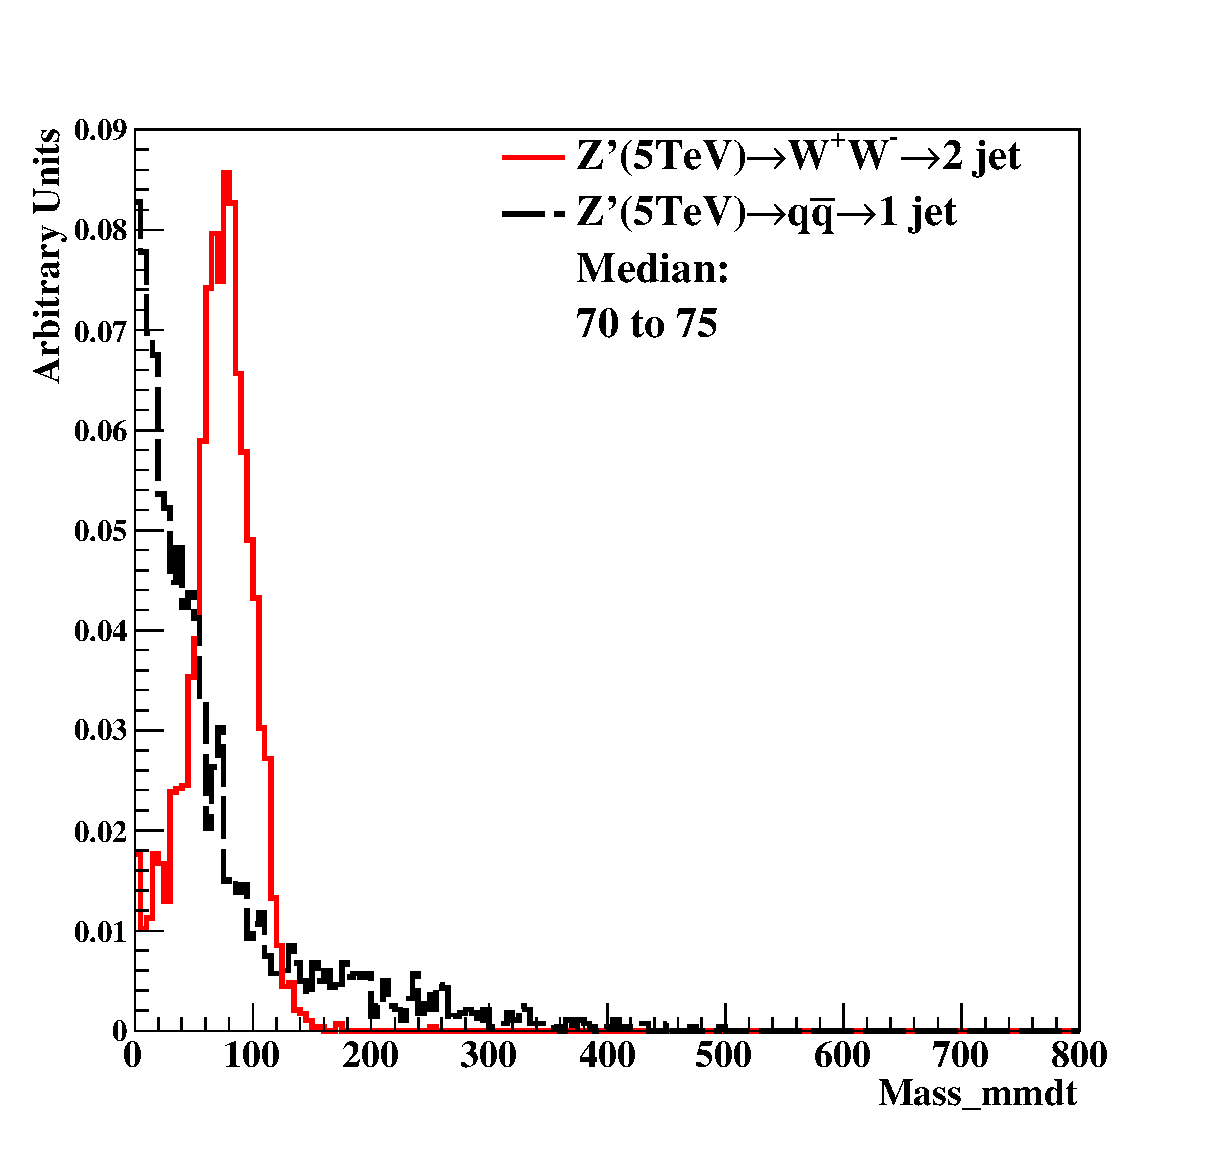
\includegraphics[width=0.22\textwidth]{figs/Dis_cluster_010_mass_mmdt_5tev_04_no_UOF.eps}
   }
      \subfigure[10~TeV at 20$\times$20 (cm$\times$cm) with cluster] {
   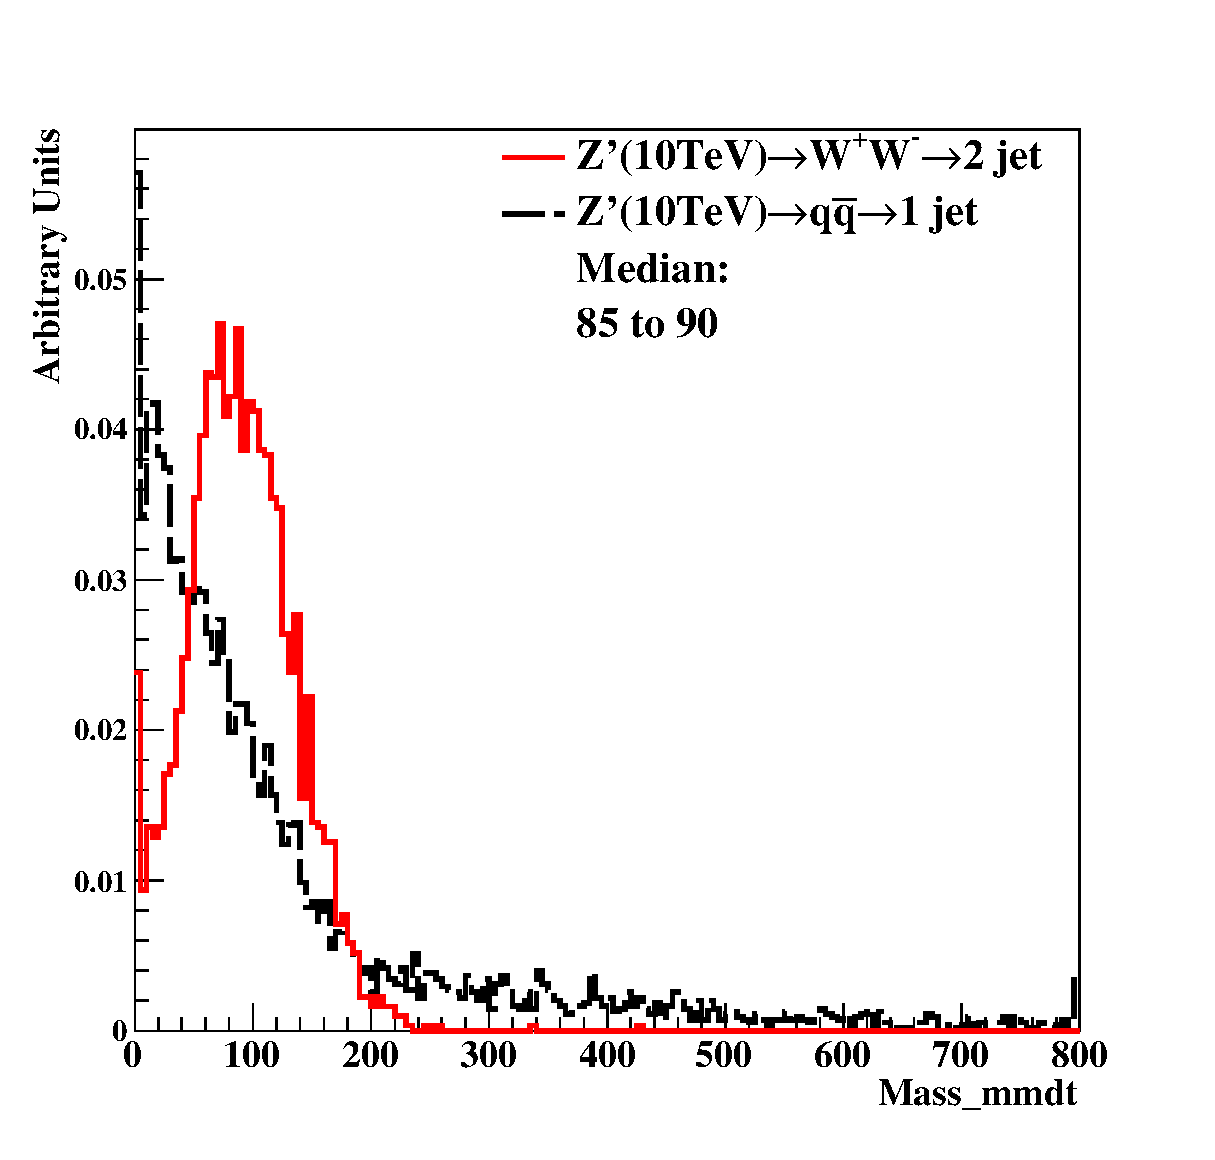
\includegraphics[width=0.22\textwidth]{figs/Dis_cluster_010_mass_mmdt_10tev_04_no_UOF.eps}
   }
   \subfigure[20~TeV at 20$\times$20 (cm$\times$cm) with cluster] {
   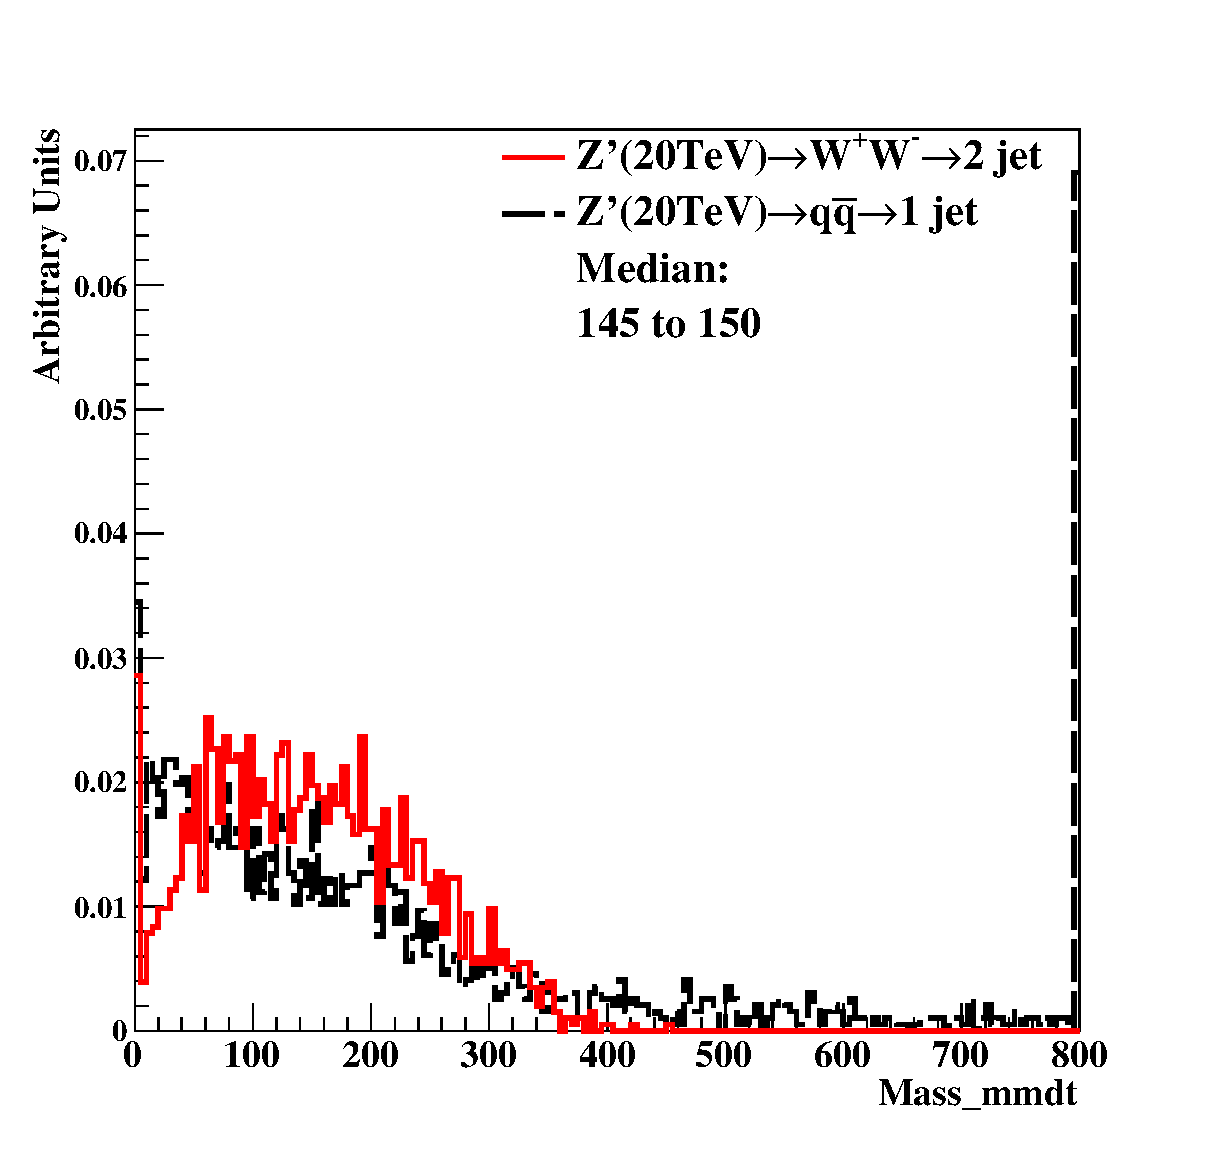
\includegraphics[width=0.22\textwidth]{figs/Dis_cluster_010_mass_mmdt_20tev_04_no_UOF.eps}
   }
    \subfigure[40~TeV at 20$\times$20 (cm$\times$cm) with cluster] {
   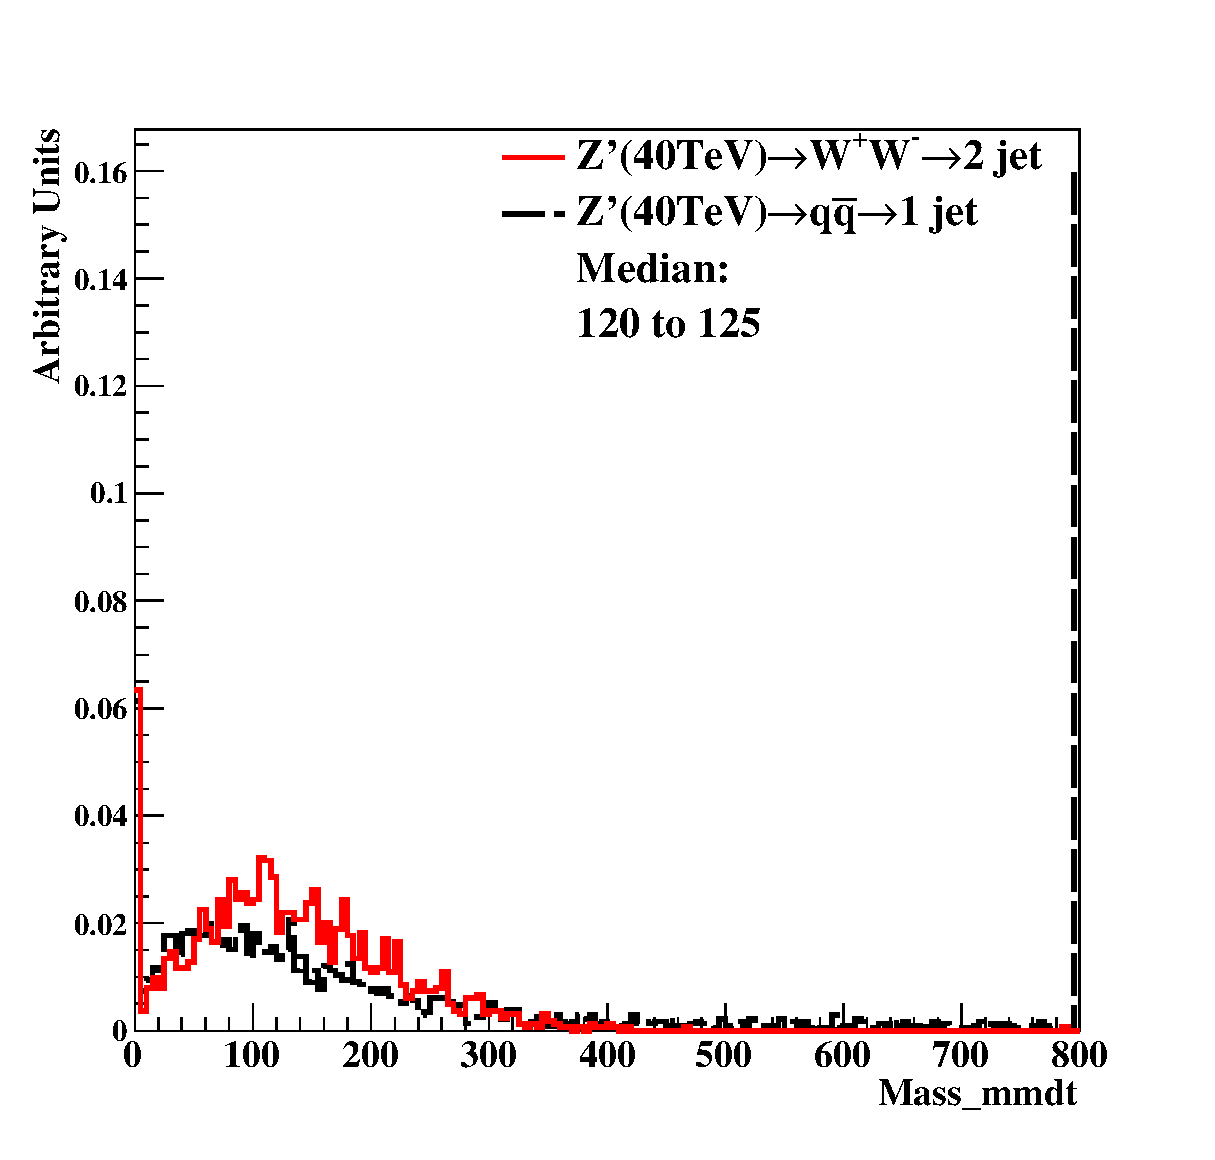
\includegraphics[width=0.22\textwidth]{figs/Dis_cluster_010_mass_mmdt_40tev_04_no_UOF.eps}
   }
   \subfigure[5~TeV at 5$\times$5 (cm$\times$cm) with cluster] {
   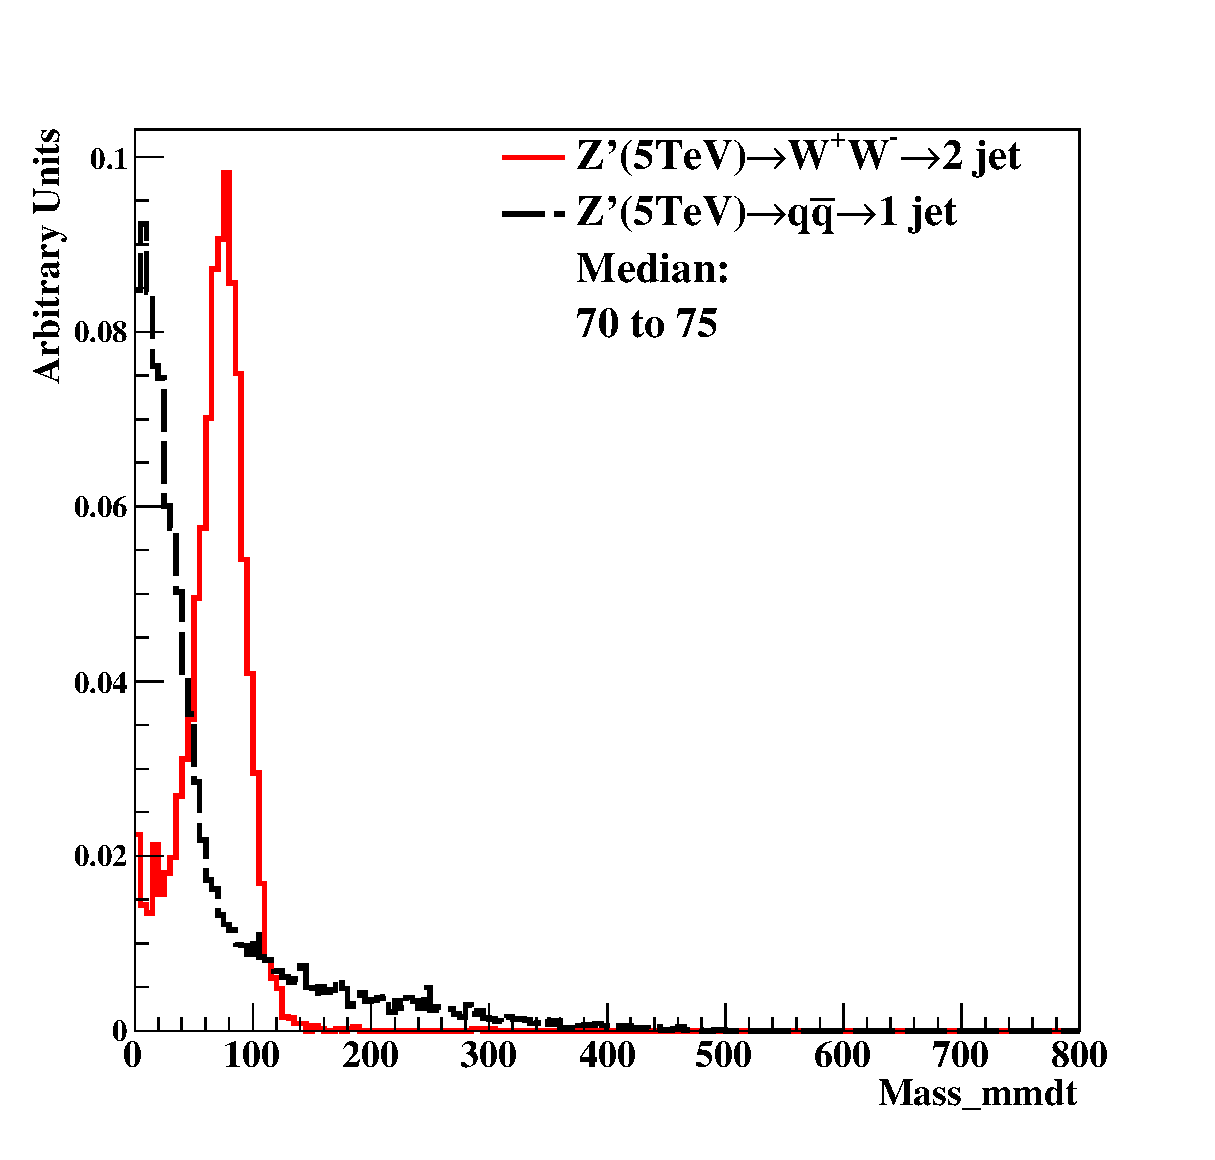
\includegraphics[width=0.22\textwidth]{figs/Dis_cluster_009_mass_mmdt_5tev_04_no_UOF.eps}
   }
   \subfigure[10~TeV at 5$\times$5 (cm$\times$cm) with cluster] {
   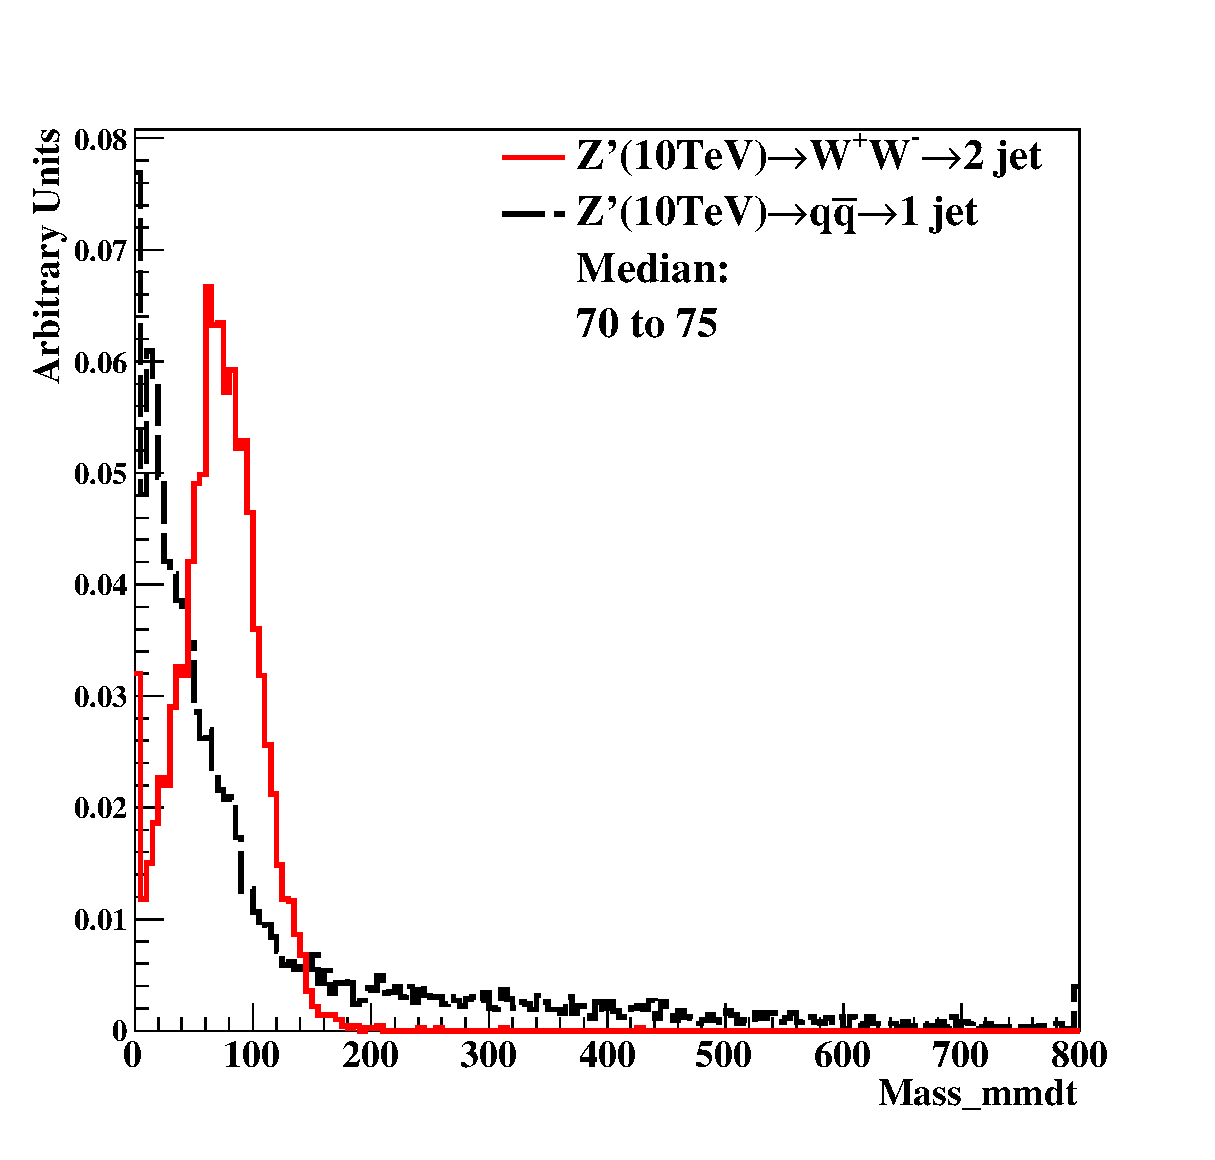
\includegraphics[width=0.22\textwidth]{figs/Dis_cluster_009_mass_mmdt_10tev_04_no_UOF.eps}
   }
      \subfigure[20~TeV at 5$\times$5 (cm$\times$cm) with cluster] {
   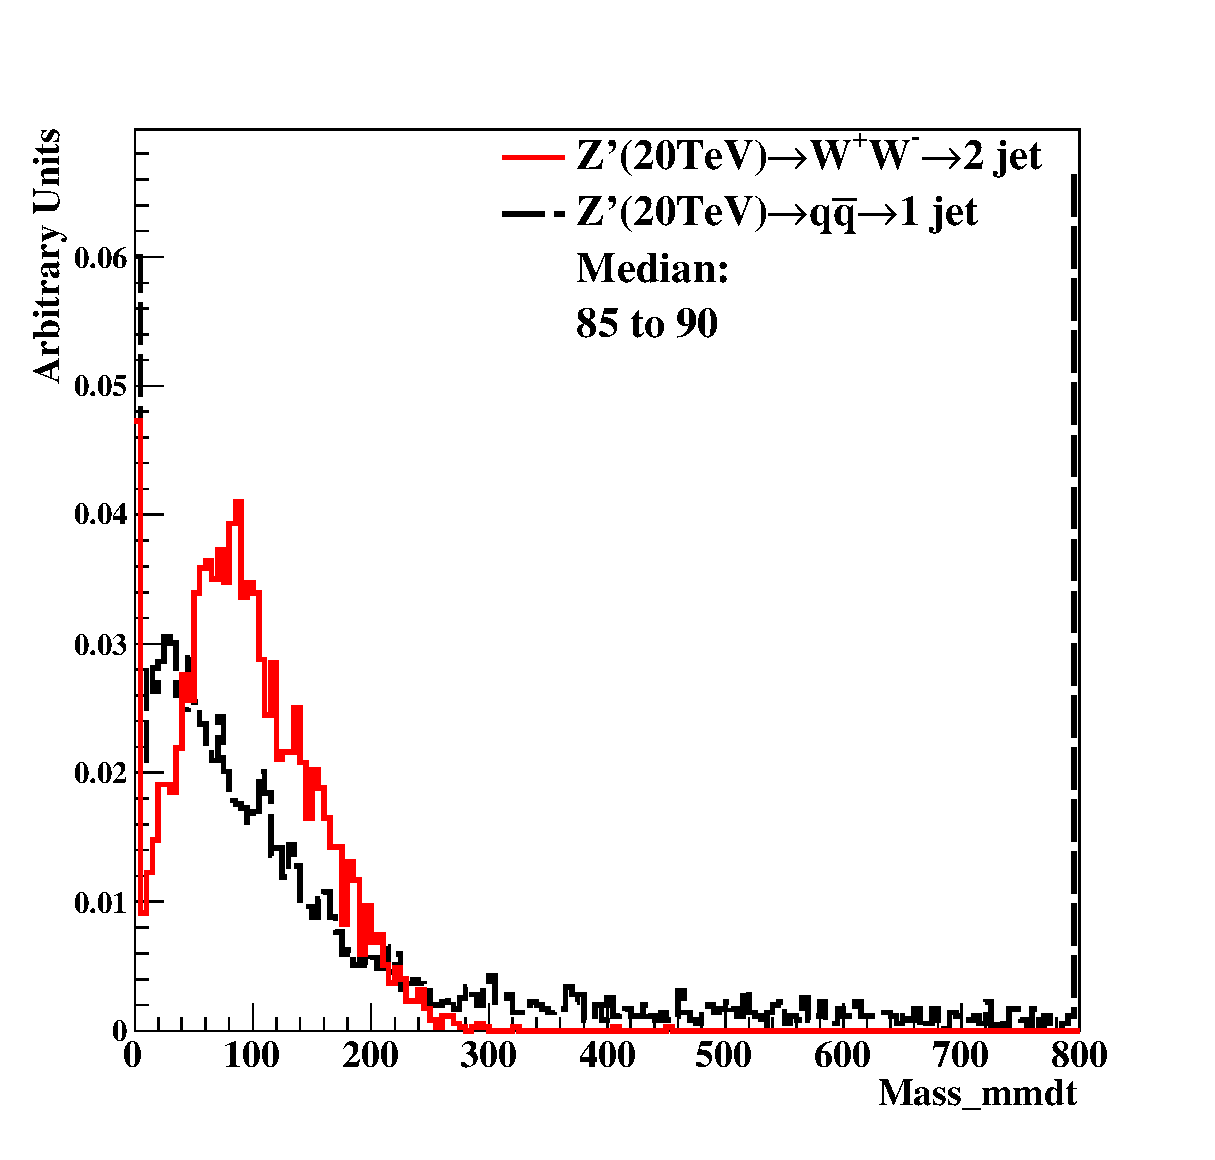
\includegraphics[width=0.22\textwidth]{figs/Dis_cluster_009_mass_mmdt_20tev_04_no_UOF.eps}\hfill
   }
      \subfigure[40~TeV at 5$\times$5 (cm$\times$cm) with cluster] {
   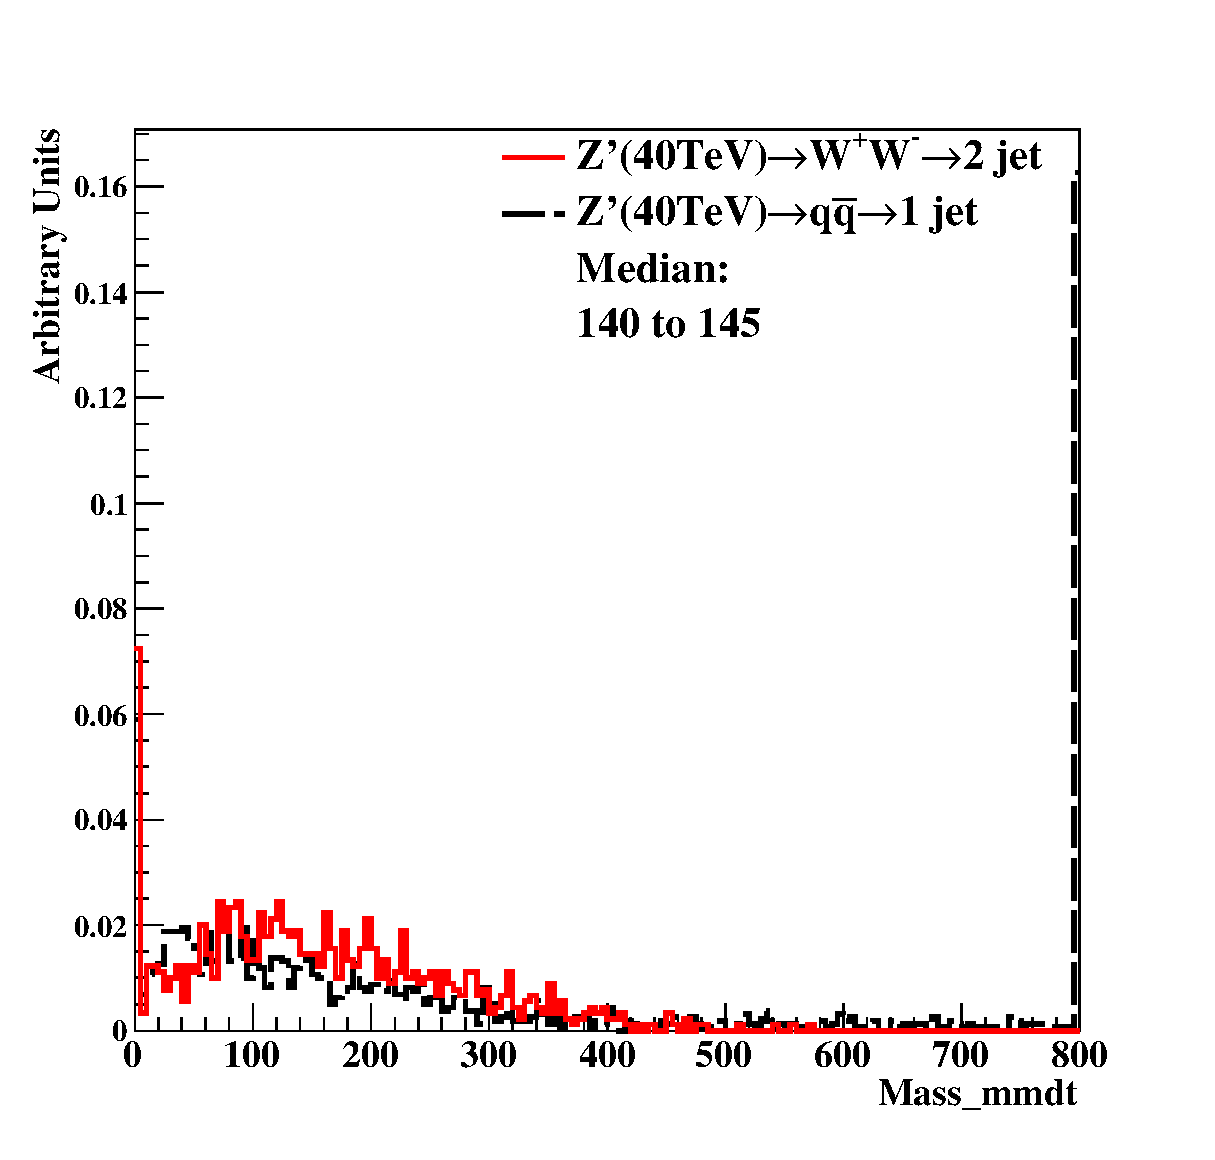
\includegraphics[width=0.22\textwidth]{figs/Dis_cluster_009_mass_mmdt_40tev_04_no_UOF.eps}\hfill
   }
   \subfigure[5~TeV at 1$\times$1 (cm$\times$cm) with cluster] {
   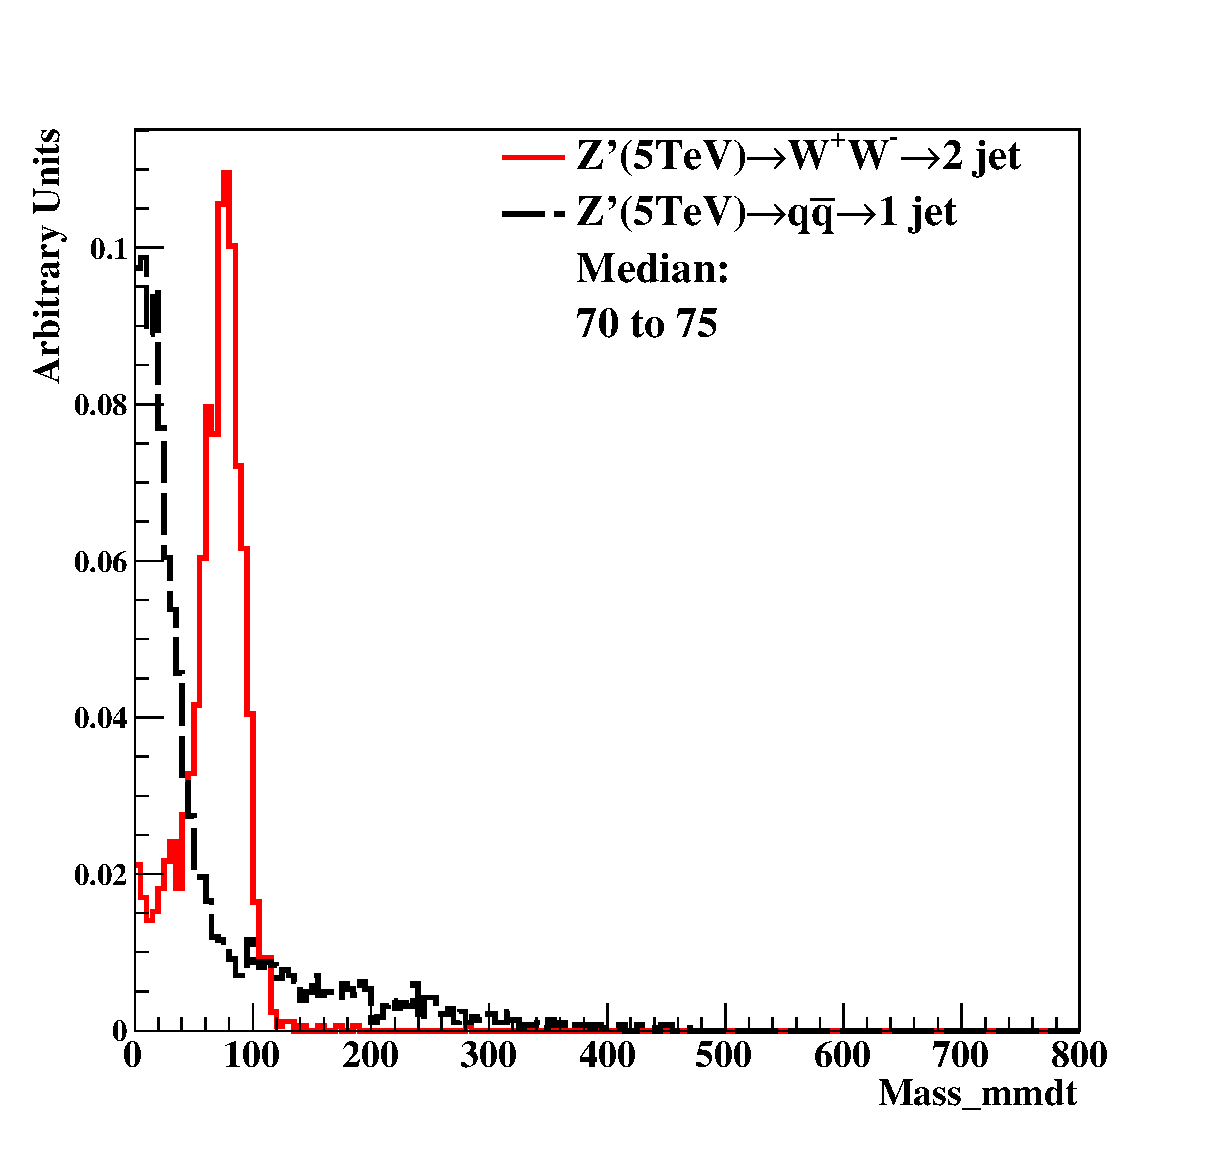
\includegraphics[width=0.22\textwidth]{figs/Dis_cluster_012_mass_mmdt_5tev_04_no_UOF.eps}\hfill
   }
    \subfigure[10~TeV at 1$\times$1 (cm$\times$cm) with cluster] {
   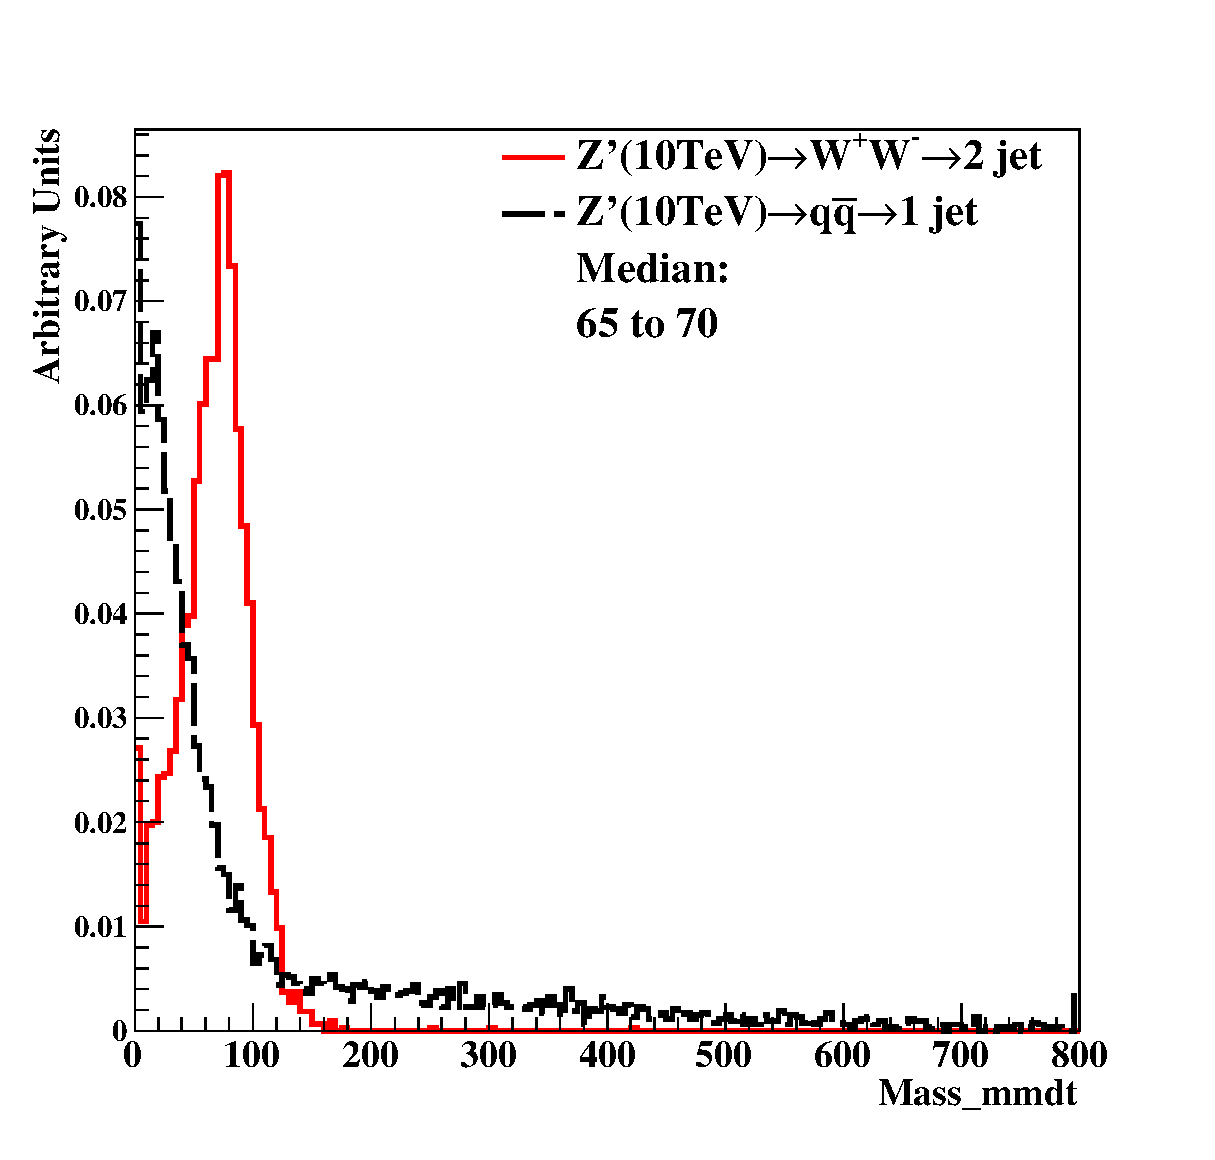
\includegraphics[width=0.22\textwidth]{figs/Dis_cluster_012_mass_mmdt_10tev_04_no_UOF.eps}
   }
   \subfigure[20~TeV at 1$\times$1 (cm$\times$cm) with cluster] {
   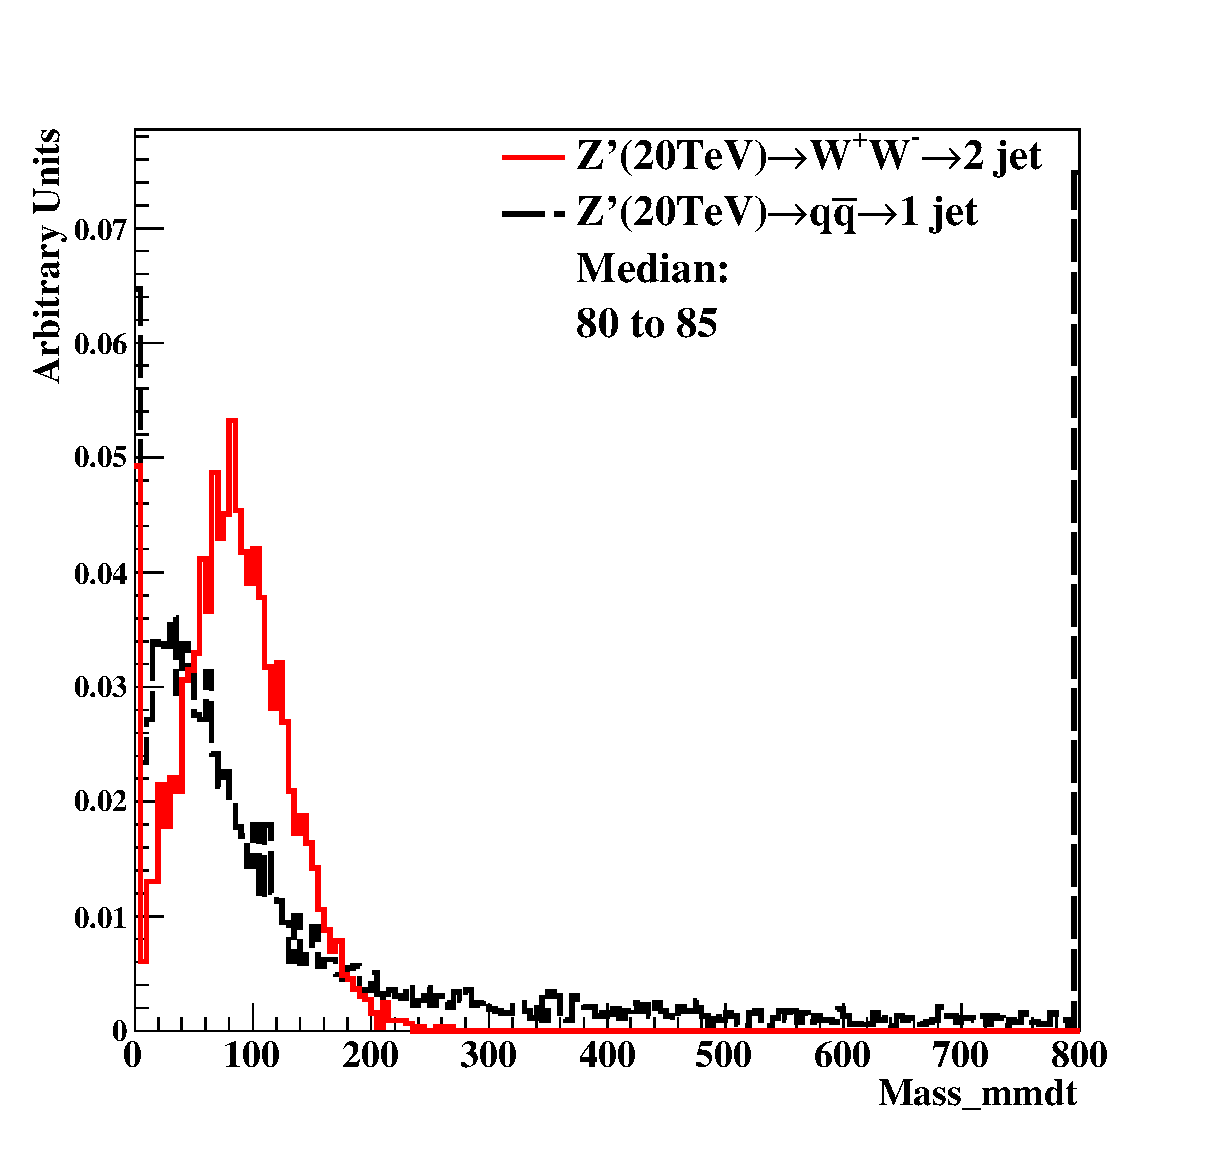
\includegraphics[width=0.22\textwidth]{figs/Dis_cluster_012_mass_mmdt_20tev_04_no_UOF.eps}\hfill
   }
      \subfigure[40~TeV at 1$\times$1 (cm$\times$cm) with cluster] {
   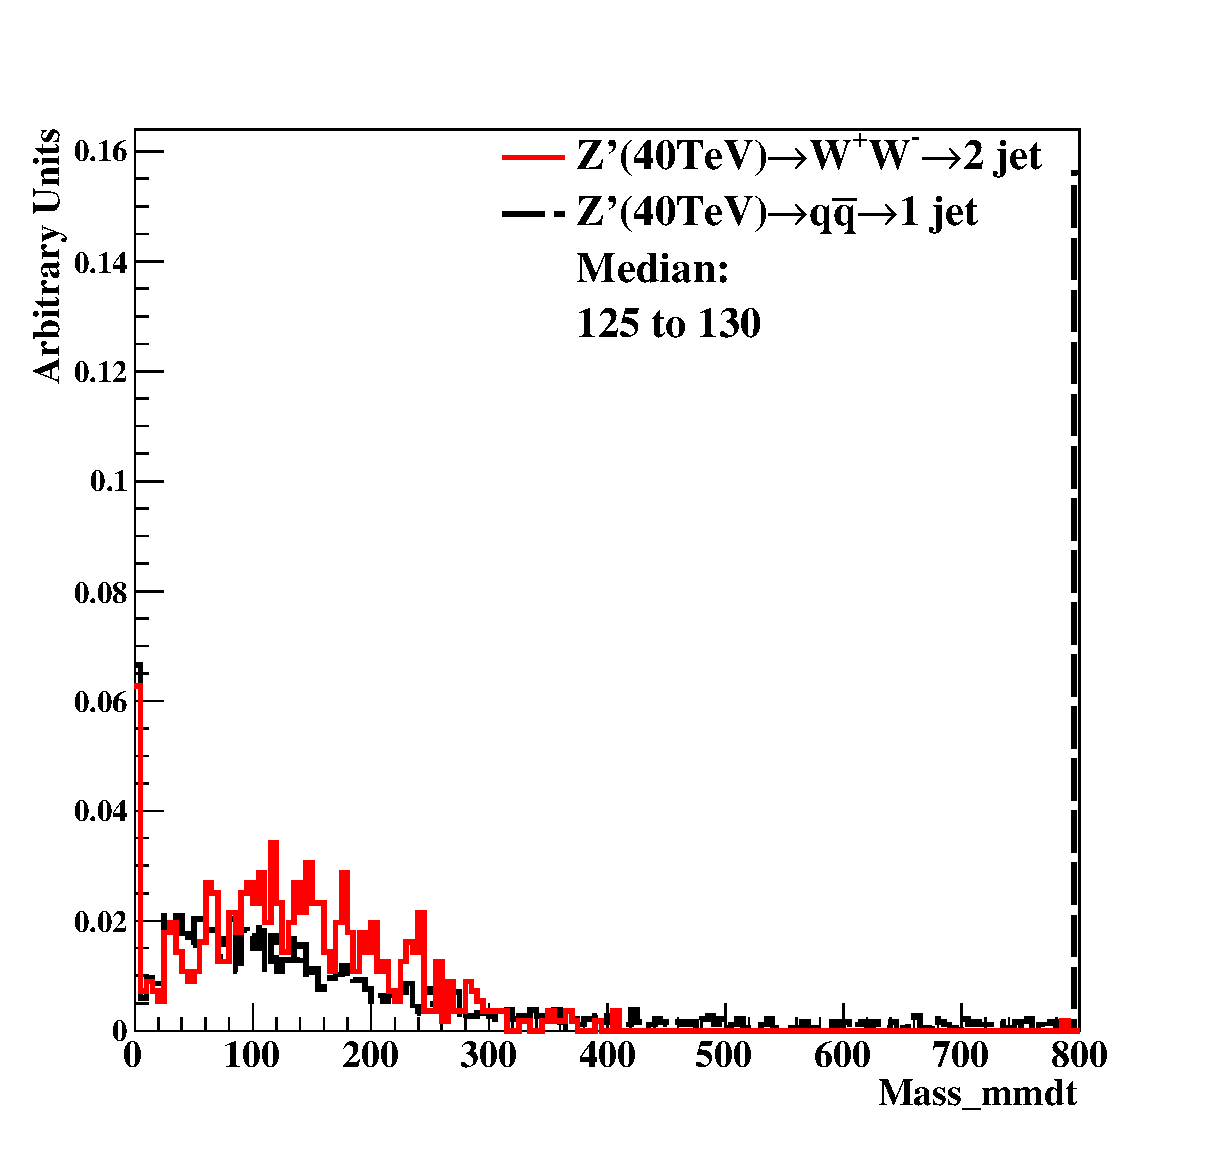
\includegraphics[width=0.22\textwidth]{figs/Dis_cluster_012_mass_mmdt_40tev_04_no_UOF.eps}
   }

\end{center}
\caption{Distributions of soft drop mass for $\beta$=0, with 5, 10, 20, and 
40~TeV c.m. energies and three different detector cell sizes: 20$\times$20, 
5$\times$5, and 1$\times$1 (cm$\times$cm). The signal (background) process is 
Z'$\rightarrow$WW (Z'$\rightarrow$q$\bar{\mathrm{q}}$).
\label{fig:cluster_mass_mmdt_ww}}
\end{figure}


\begin{figure}
\begin{center}
  \subfigure[Central at Median($20\times20$=,$5\times5$=,$1\times1$=) change width with cluster at 5~TeV] {
  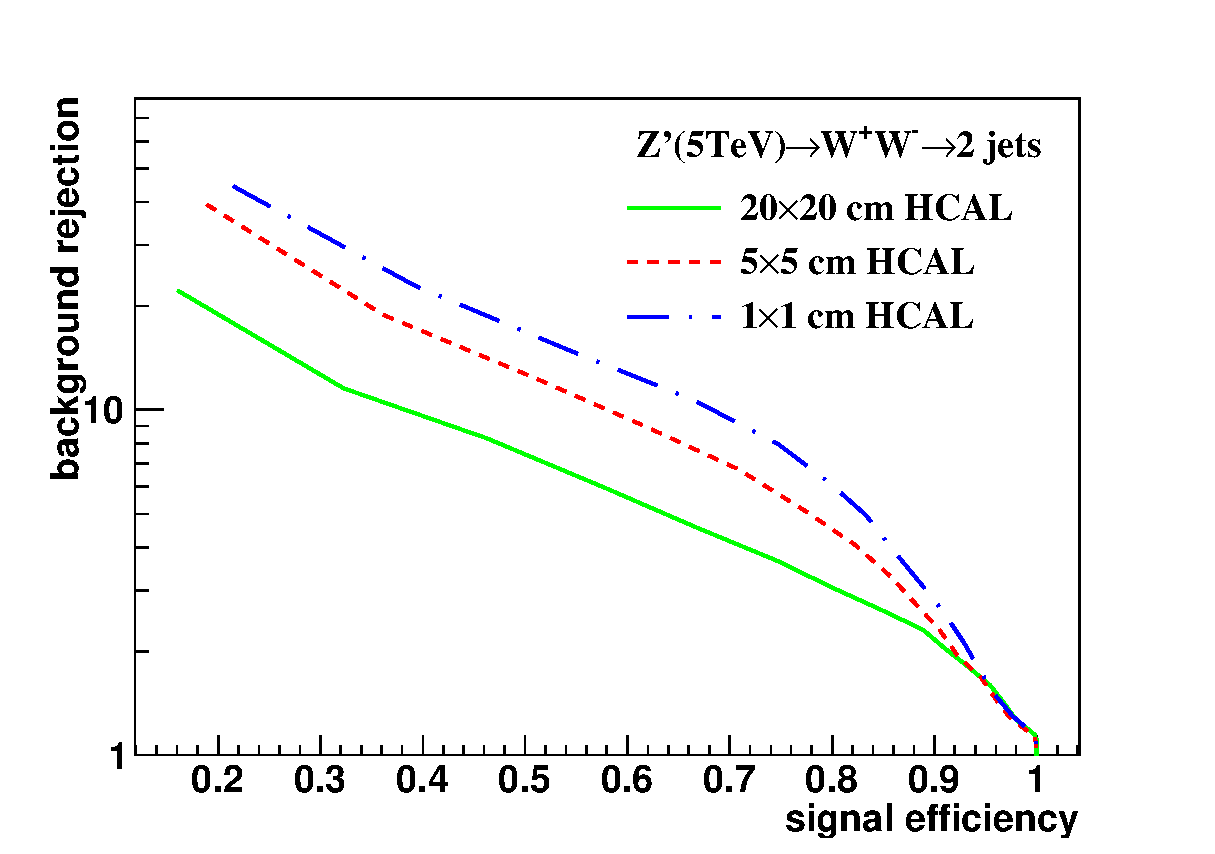
\includegraphics[width=0.43\textwidth]{figs/A_Cluster_mass_mmdt_5tev_eff_1_central_fix_at_Median_bin_ww_qq_log_no_UOF.eps}
  }
  \subfigure[Central at Median($20\times20$=,$5\times5$=,$1\times1$=) change width with cluster at 10~TeV] {
  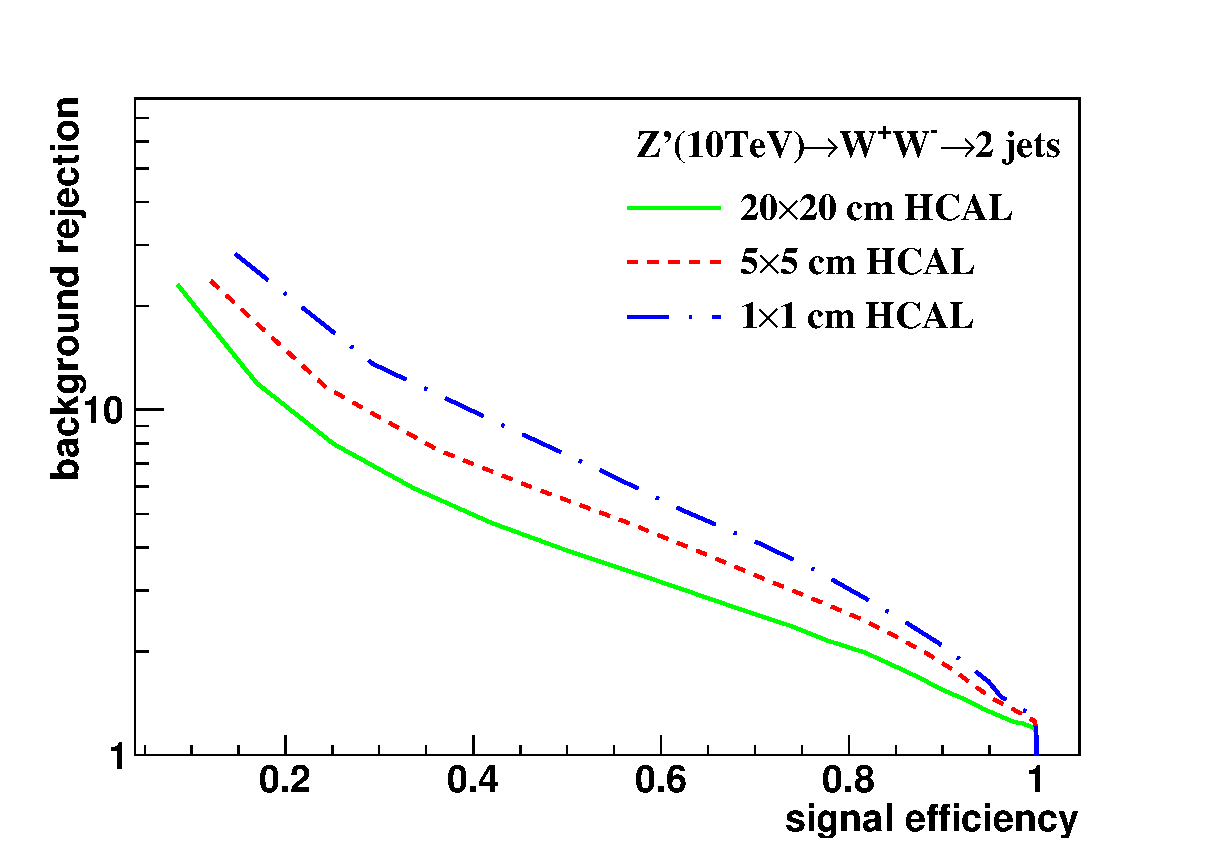
\includegraphics[width=0.43\textwidth]{figs/A_Cluster_mass_mmdt_10tev_eff_1_central_fix_at_Median_bin_ww_qq_log_no_UOF.eps}
  }
 \subfigure[Central at Median($20\times20$=,$5\times5$=,$1\times1$=) change width with cluster at 20~TeV] {
 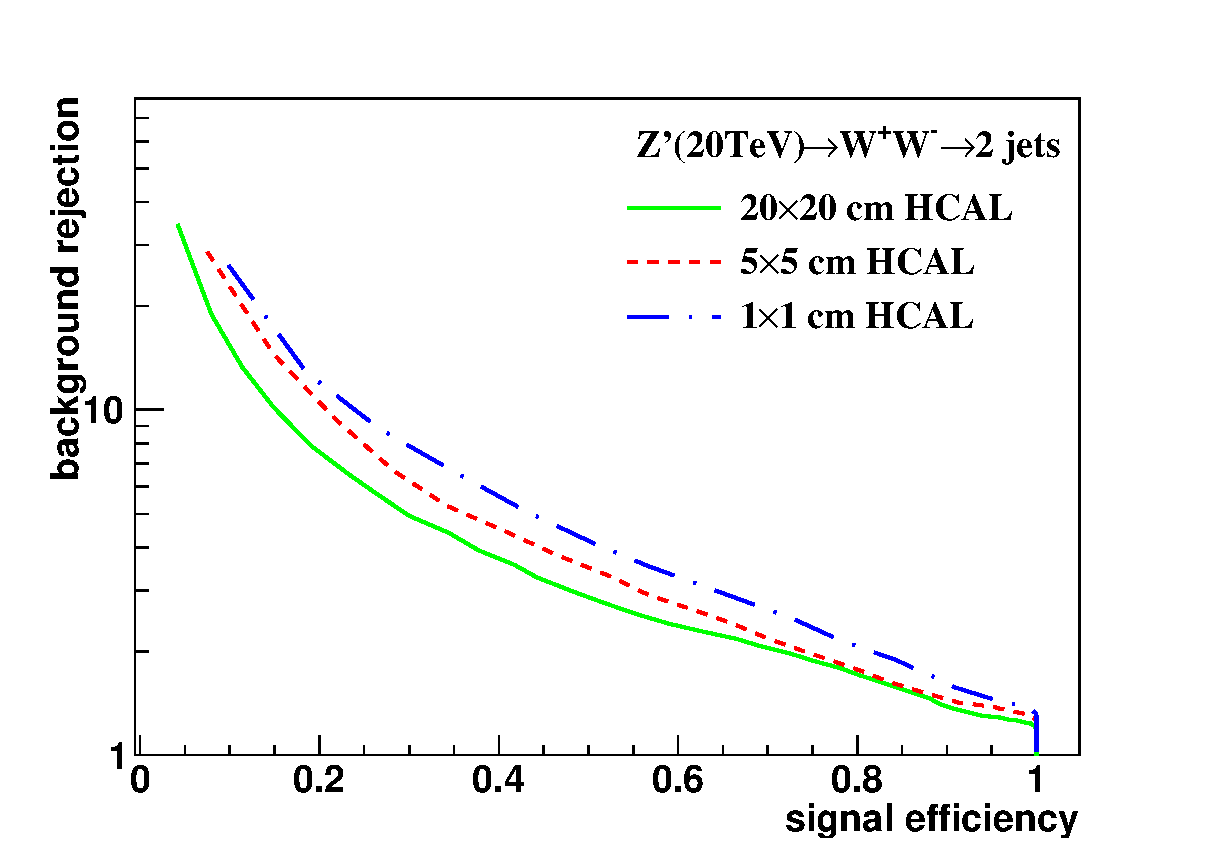
\includegraphics[width=0.43\textwidth]{figs/A_Cluster_mass_mmdt_20tev_eff_1_central_fix_at_Median_bin_ww_qq_log_no_UOF.eps}
 }
 \subfigure[Central at Median($20\times20$=,$5\times5$=,$1\times1$=) change width with cluster at 40~TeV] {
 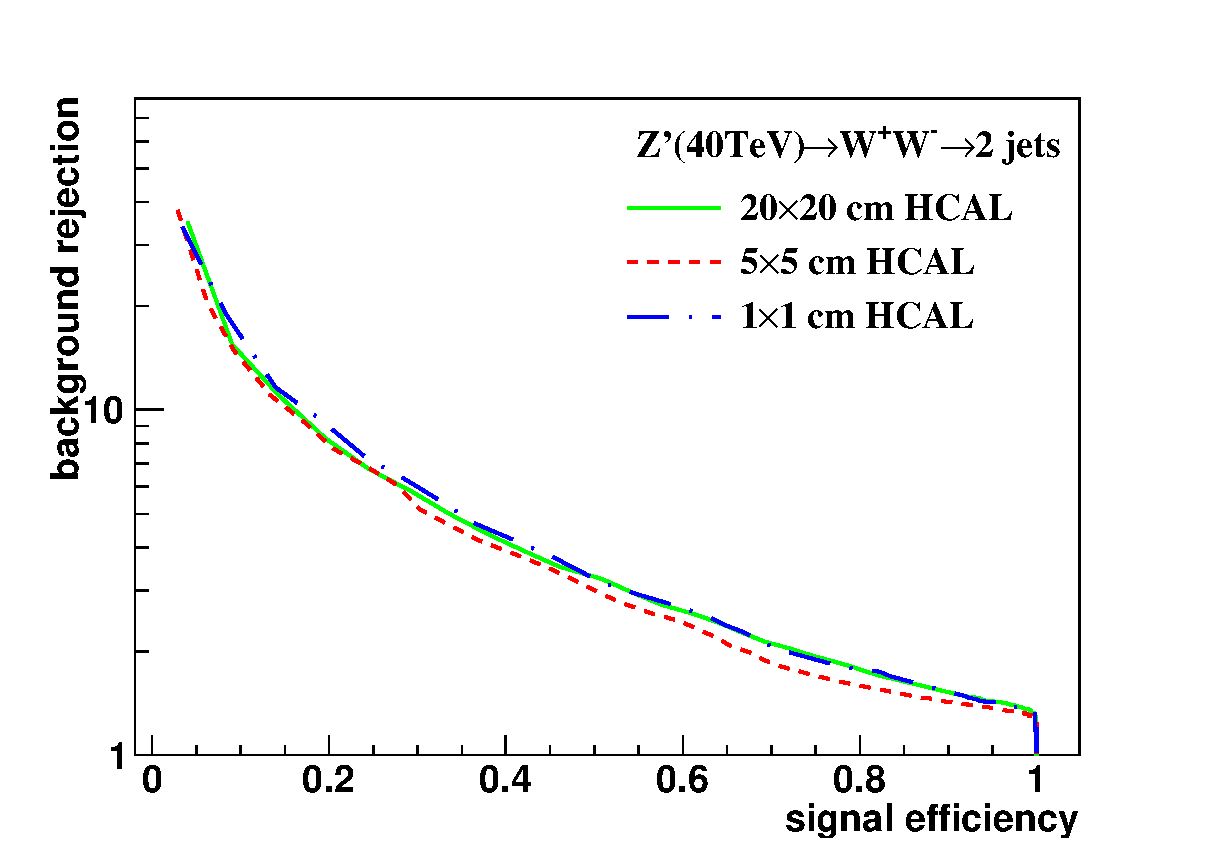
\includegraphics[width=0.43\textwidth]{figs/A_Cluster_mass_mmdt_40tev_eff_1_central_fix_at_Median_bin_ww_qq_log_no_UOF.eps}
 }
\end{center}
\caption{The ROC curves of soft drop mass selection for $\beta$=0 
with 5, 10, 20, and 40~TeV c.m. energies. 
Three different detector cell sizes are compared: 20$\times$20, 
5$\times$5, and 1$\times$1 (cm$\times$cm). 
The signal (background) process is Z'$\rightarrow$WW 
(Z'$\rightarrow$q$\bar{\mathrm{q}}$).}
\label{fig:cluster_mass_mmdt_ww_ROC}
\end{figure}


\begin{figure}
\begin{center}
   \subfigure[5~TeV at 20$\times$20 (cm$\times$cm) with cluster] {
   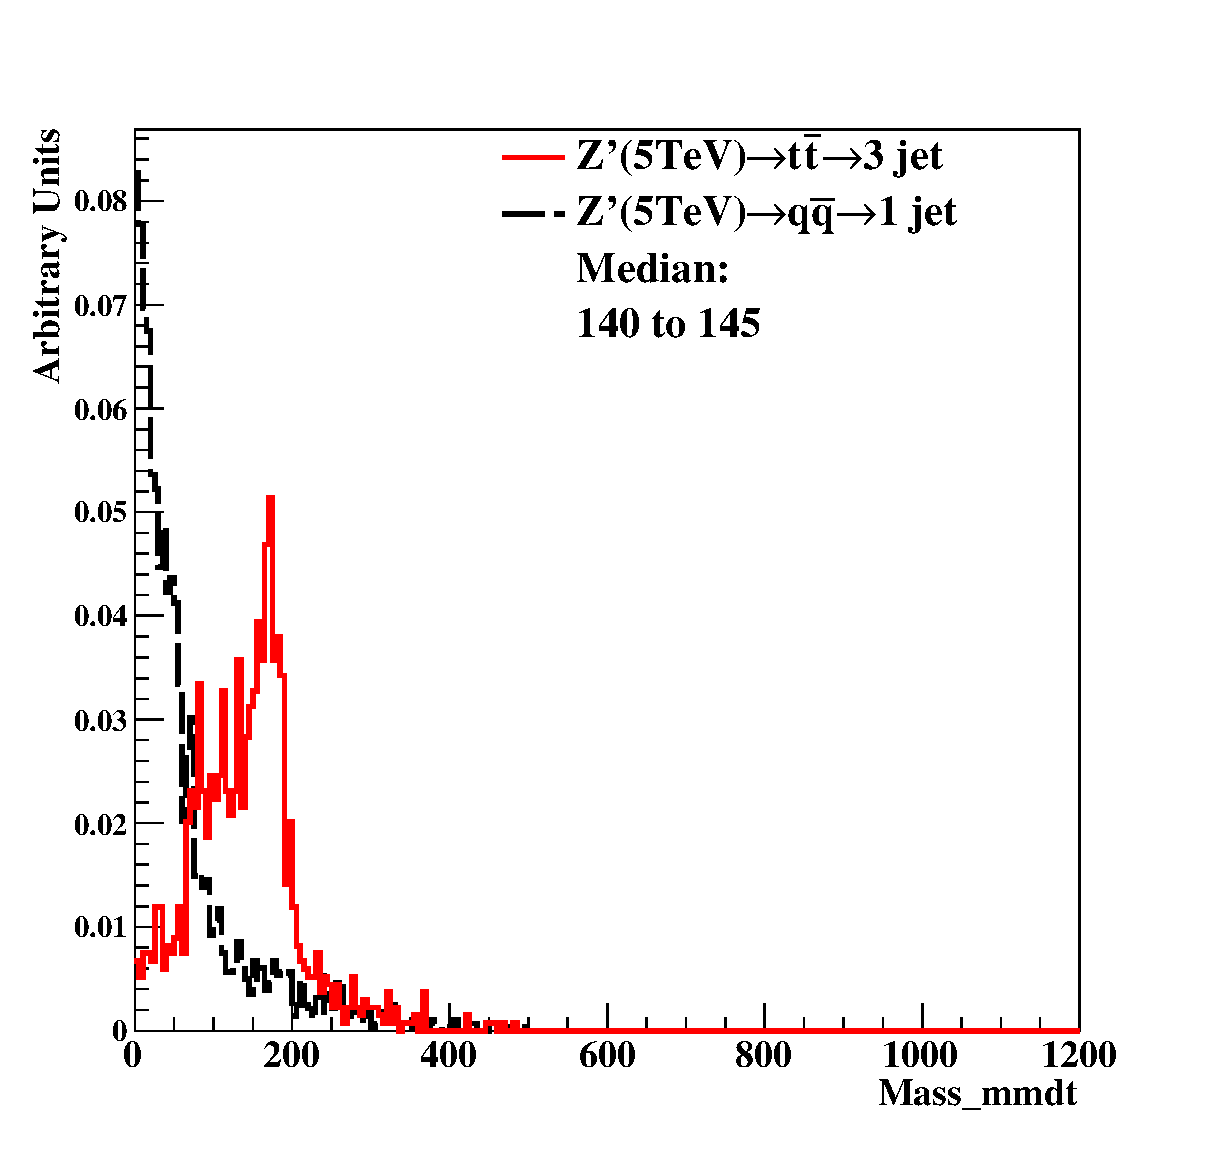
\includegraphics[width=0.22\textwidth]{figs/Dis_cluster_010_mass_mmdt_tt_5tev_04_tt_no_UOF.eps}
   }
      \subfigure[10~TeV at 20$\times$20 (cm$\times$cm) with cluster] {
   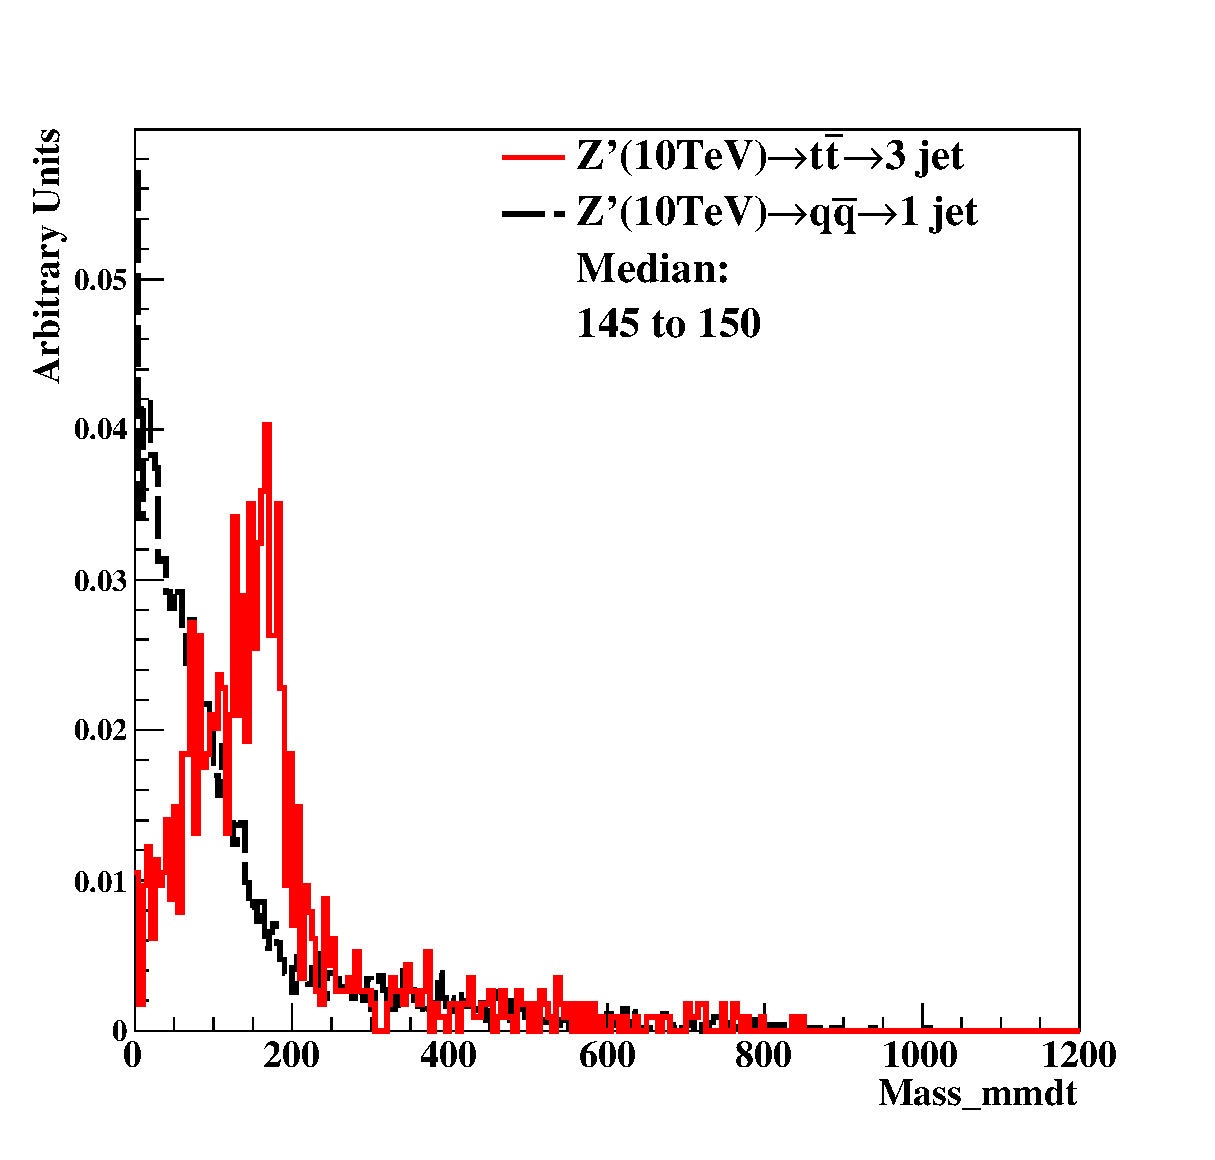
\includegraphics[width=0.22\textwidth]{figs/Dis_cluster_010_mass_mmdt_tt_10tev_04_tt_no_UOF.eps}
   }
   \subfigure[20~TeV at 5$\times$5 (cm$\times$cm) with cluster] {
   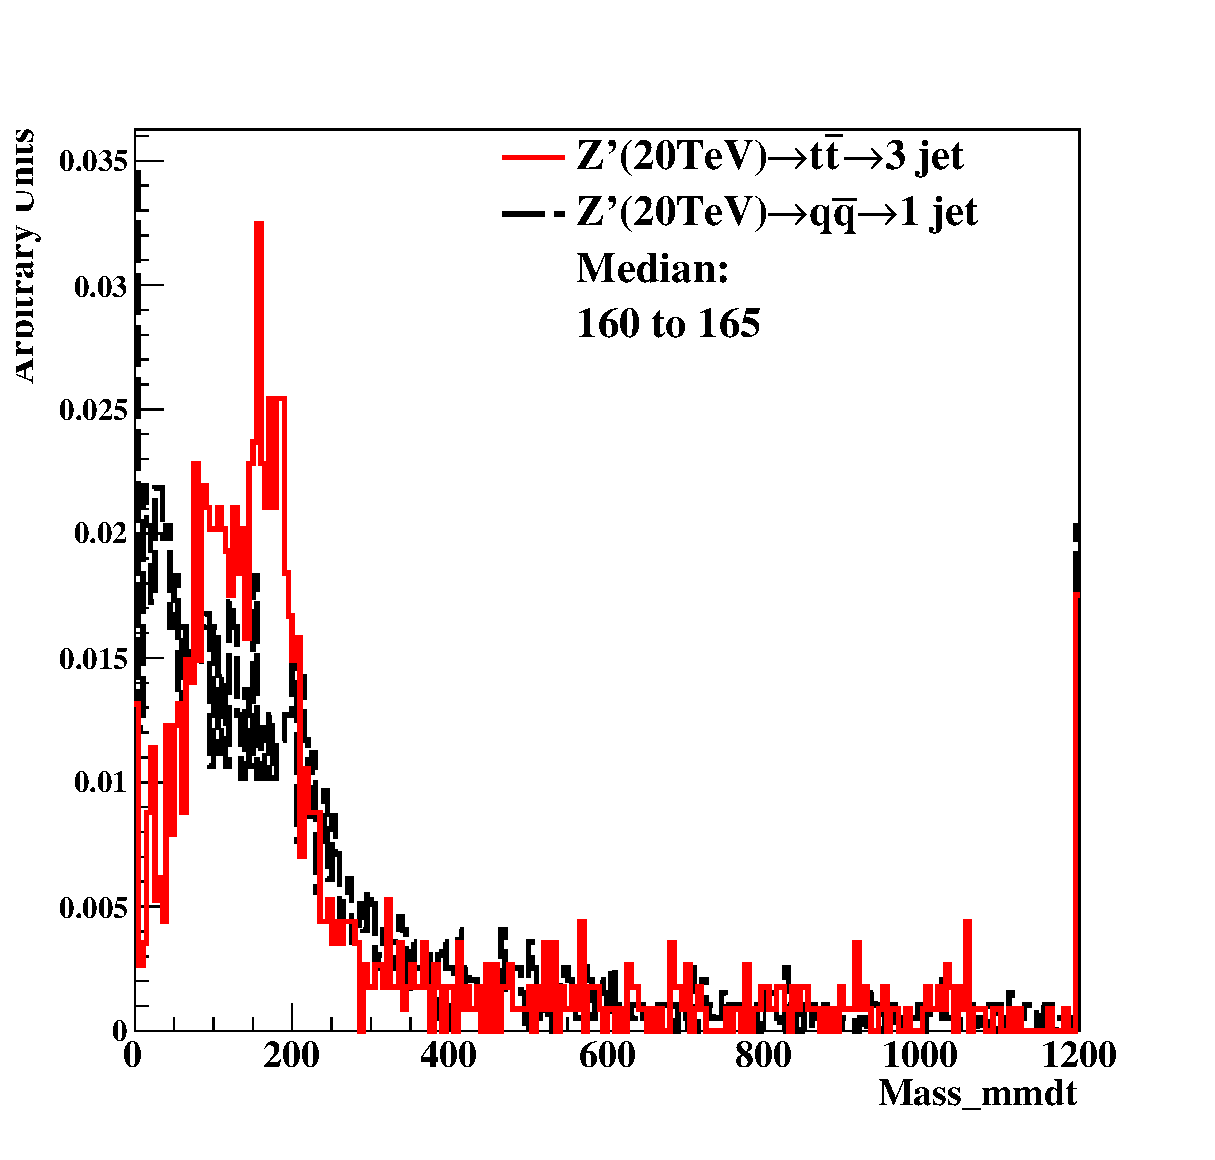
\includegraphics[width=0.22\textwidth]{figs/Dis_cluster_010_mass_mmdt_tt_20tev_04_tt_no_UOF.eps}
   }
    \subfigure[40~TeV at 5$\times$5 (cm$\times$cm) with cluster] {
   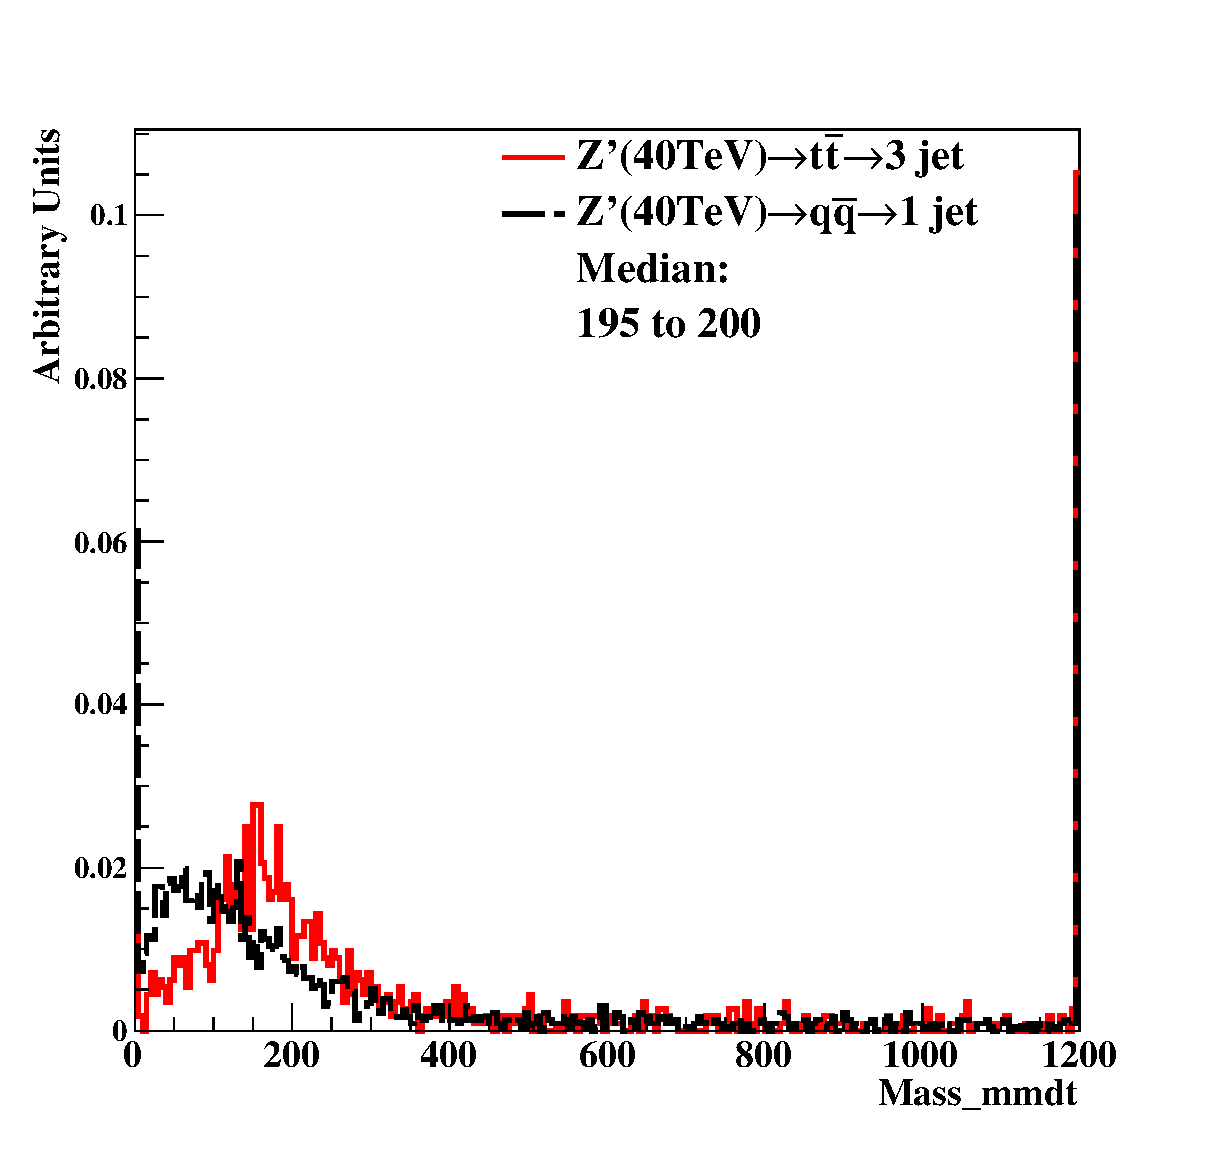
\includegraphics[width=0.22\textwidth]{figs/Dis_cluster_010_mass_mmdt_tt_40tev_04_tt_no_UOF.eps}
   }
   \subfigure[5~TeV at 1$\times$1 (cm$\times$cm) with cluster] {
   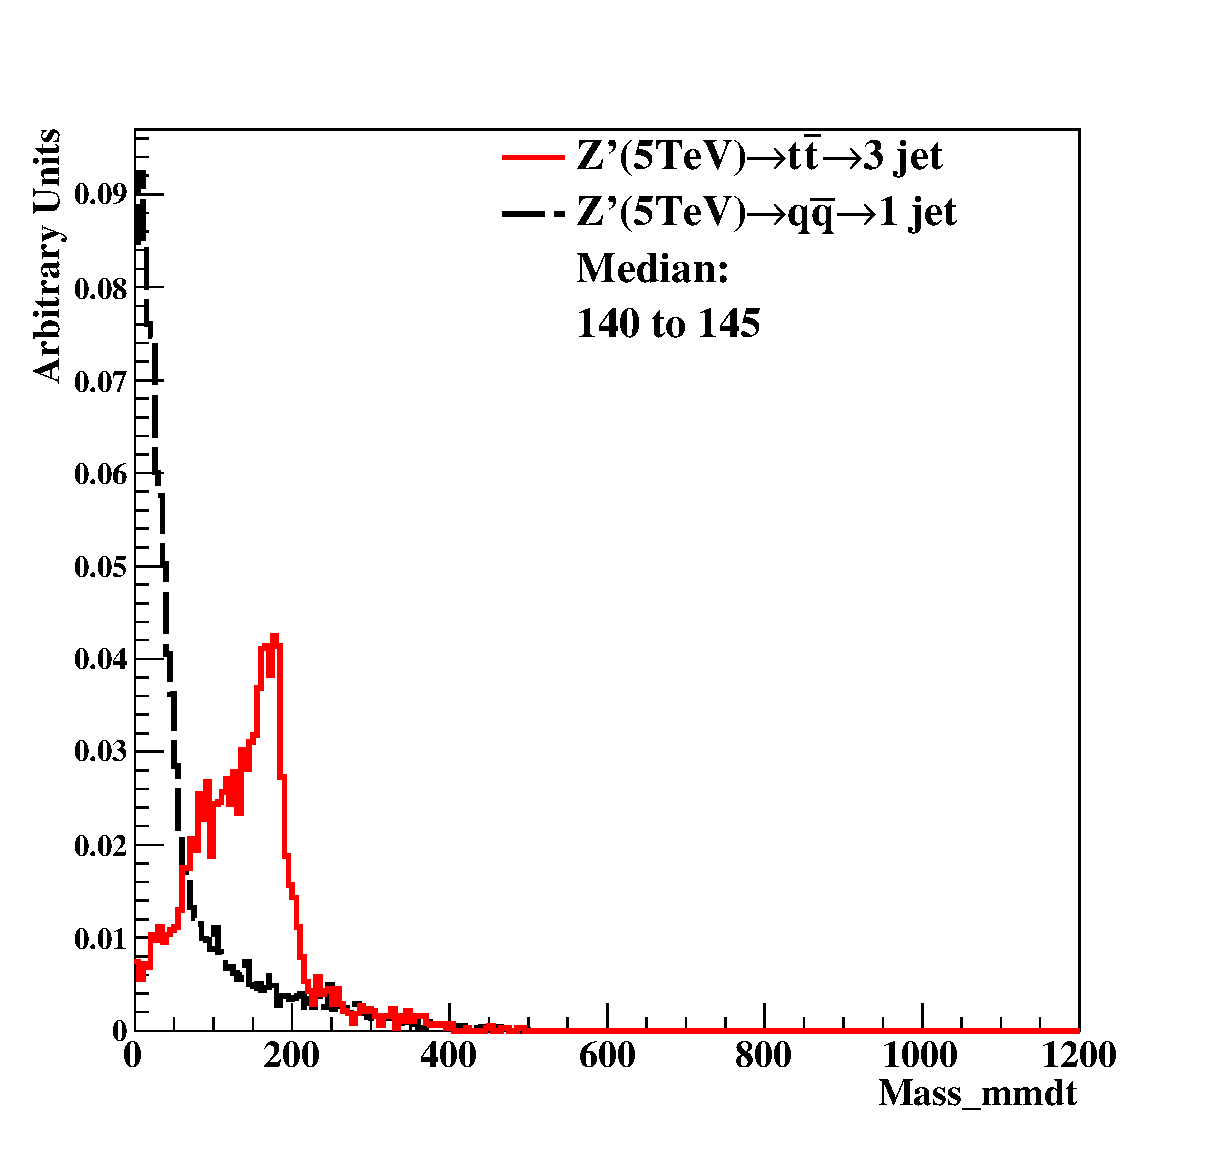
\includegraphics[width=0.22\textwidth]{figs/Dis_cluster_009_mass_mmdt_tt_5tev_04_tt_no_UOF.eps}
   }
   \subfigure[10~TeV at 1$\times$1 (cm$\times$cm) with cluster] {
   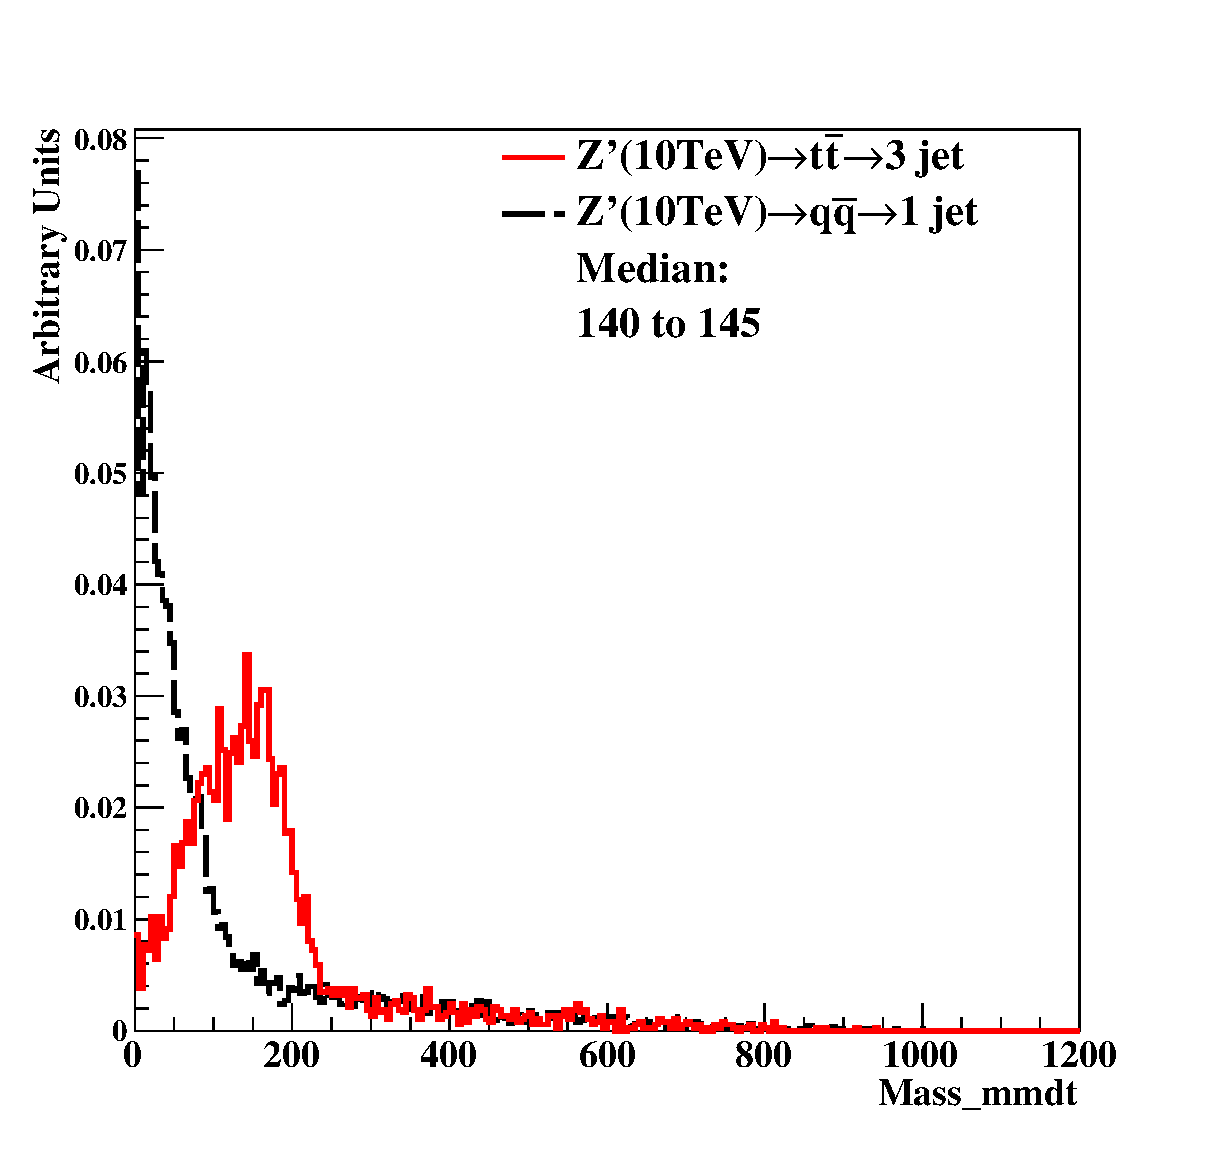
\includegraphics[width=0.22\textwidth]{figs/Dis_cluster_009_mass_mmdt_tt_10tev_04_tt_no_UOF.eps}
   }
   \subfigure[20~TeV at 20$\times$20 (cm$\times$cm) with cluster] {
   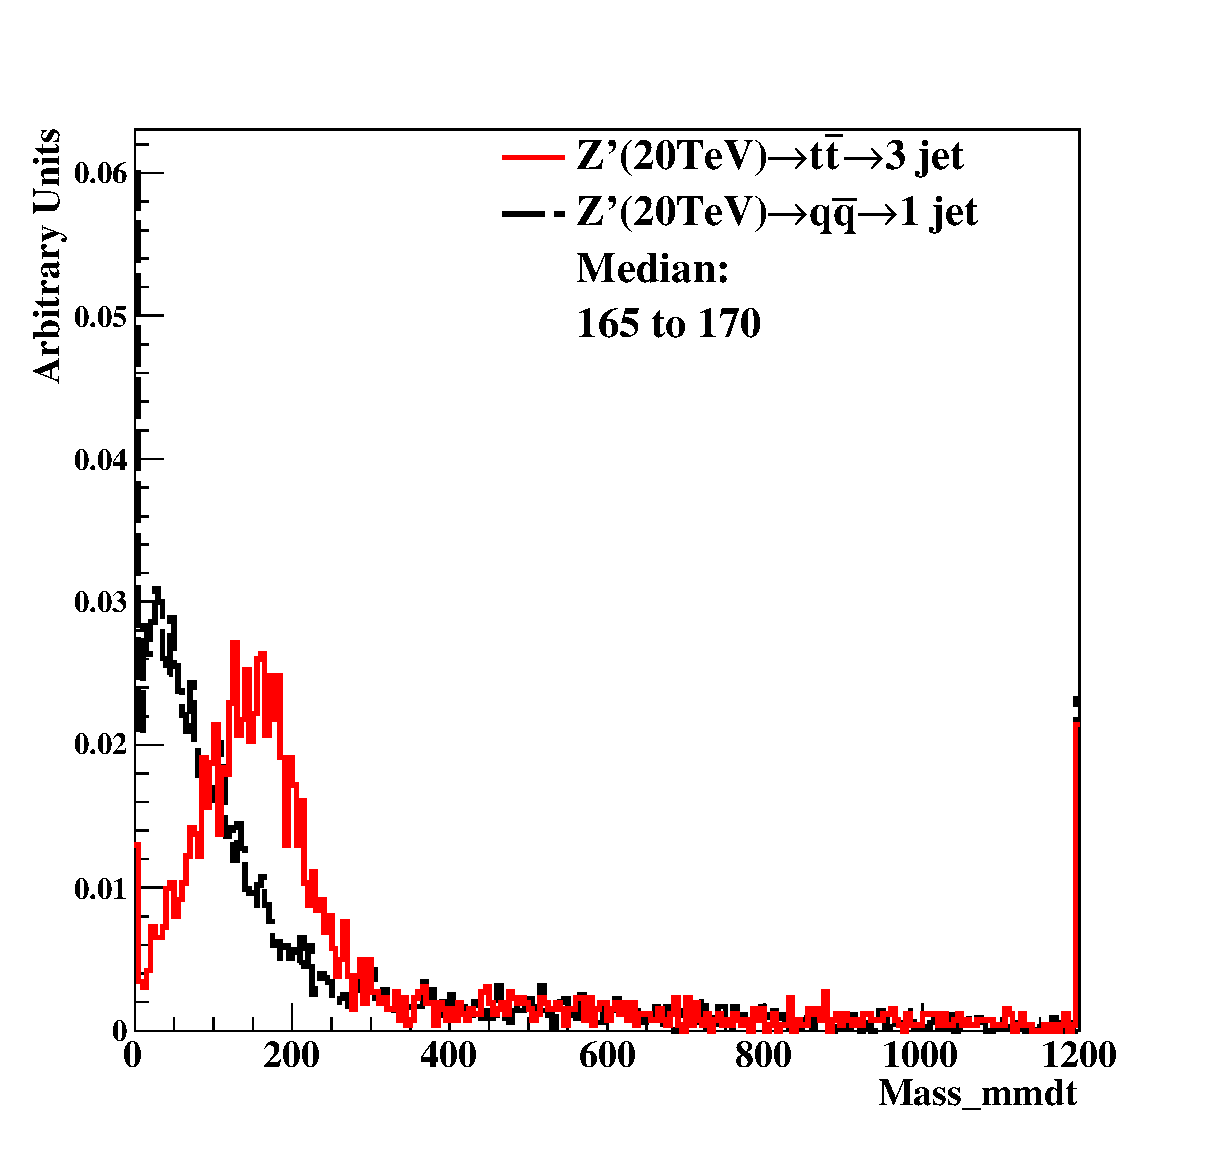
\includegraphics[width=0.22\textwidth]{figs/Dis_cluster_009_mass_mmdt_tt_20tev_04_tt_no_UOF.eps}\hfill
   }
      \subfigure[40~TeV at 20$\times$20 (cm$\times$cm) with cluster] {
   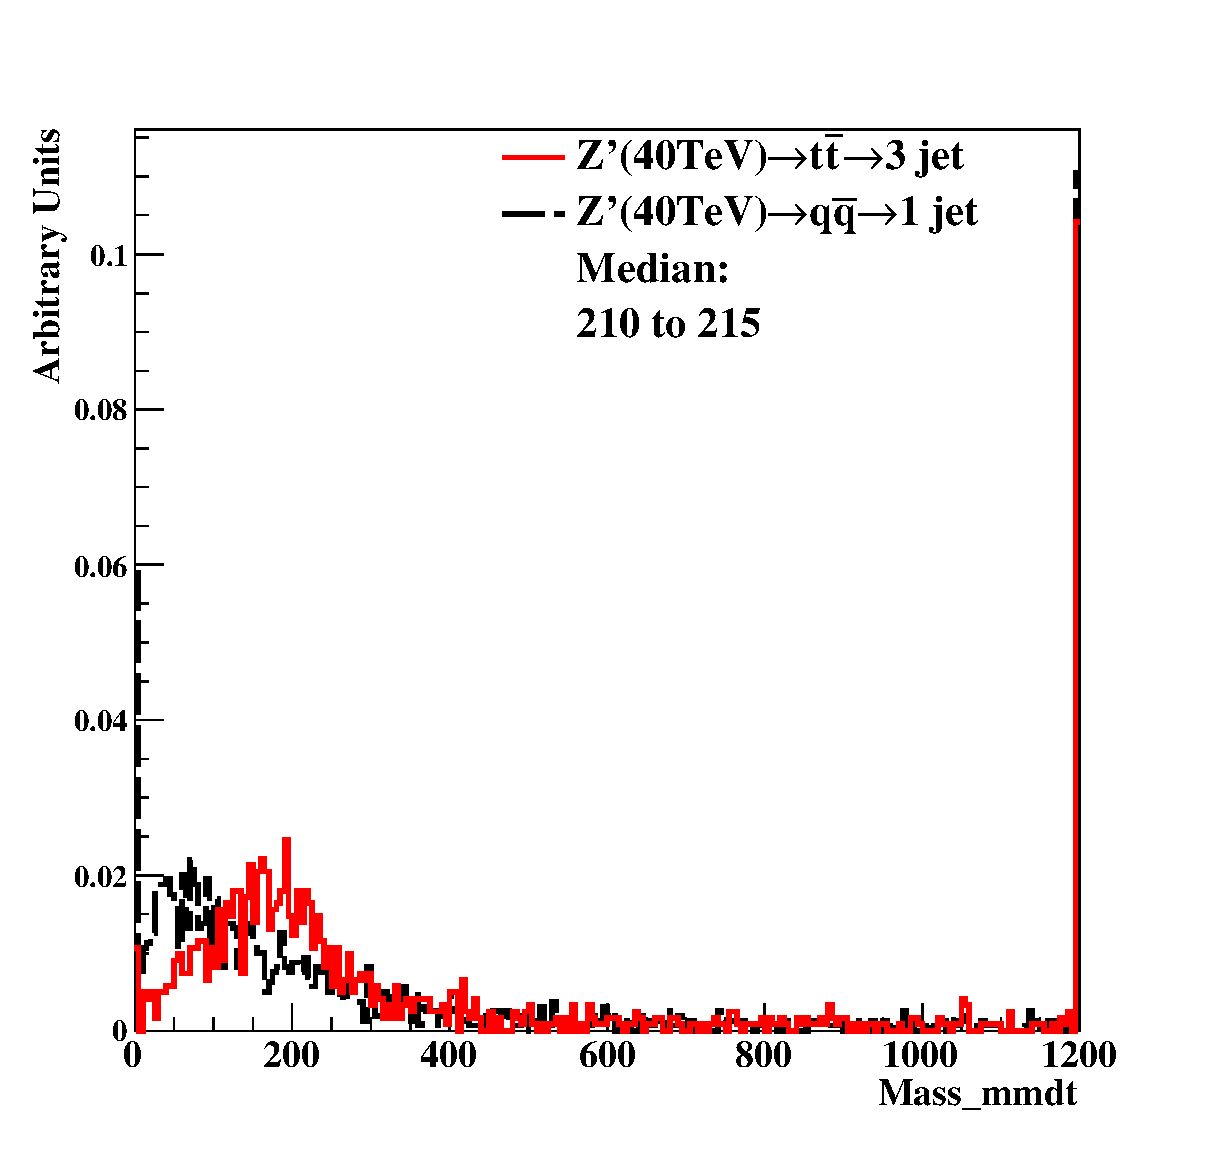
\includegraphics[width=0.22\textwidth]{figs/Dis_cluster_009_mass_mmdt_tt_40tev_04_tt_no_UOF.eps}\hfill
   }
   \subfigure[5~TeV at 5$\times$5 (cm$\times$cm) with cluster] {
   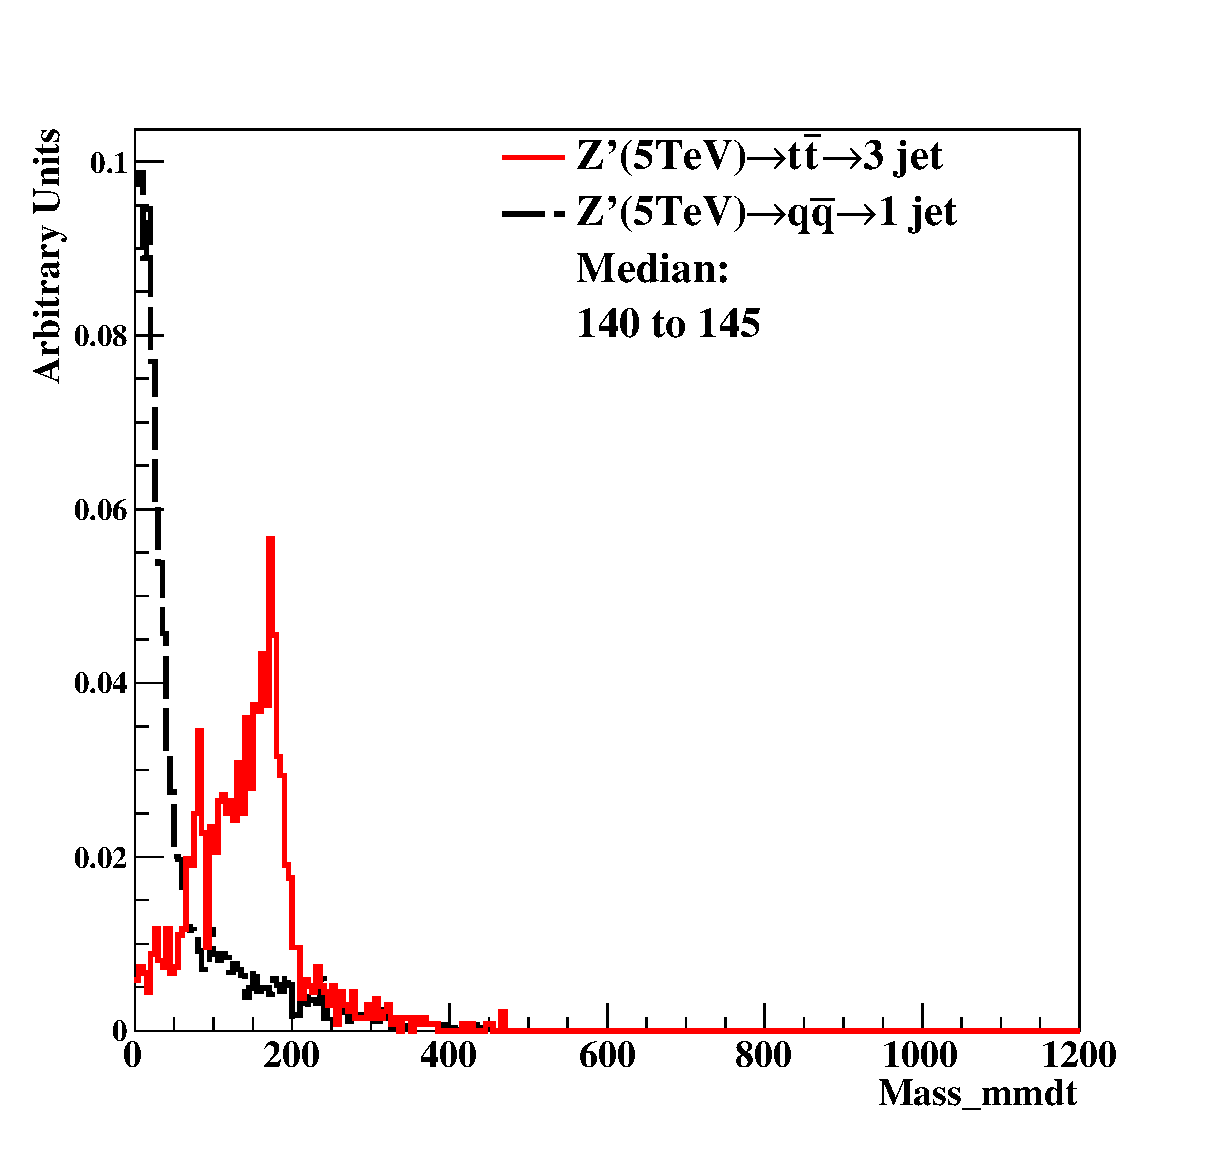
\includegraphics[width=0.22\textwidth]{figs/Dis_cluster_012_mass_mmdt_tt_5tev_04_tt_no_UOF.eps}\hfill
   }
    \subfigure[10~TeV at 5$\times$5 (cm$\times$cm) with cluster] {
   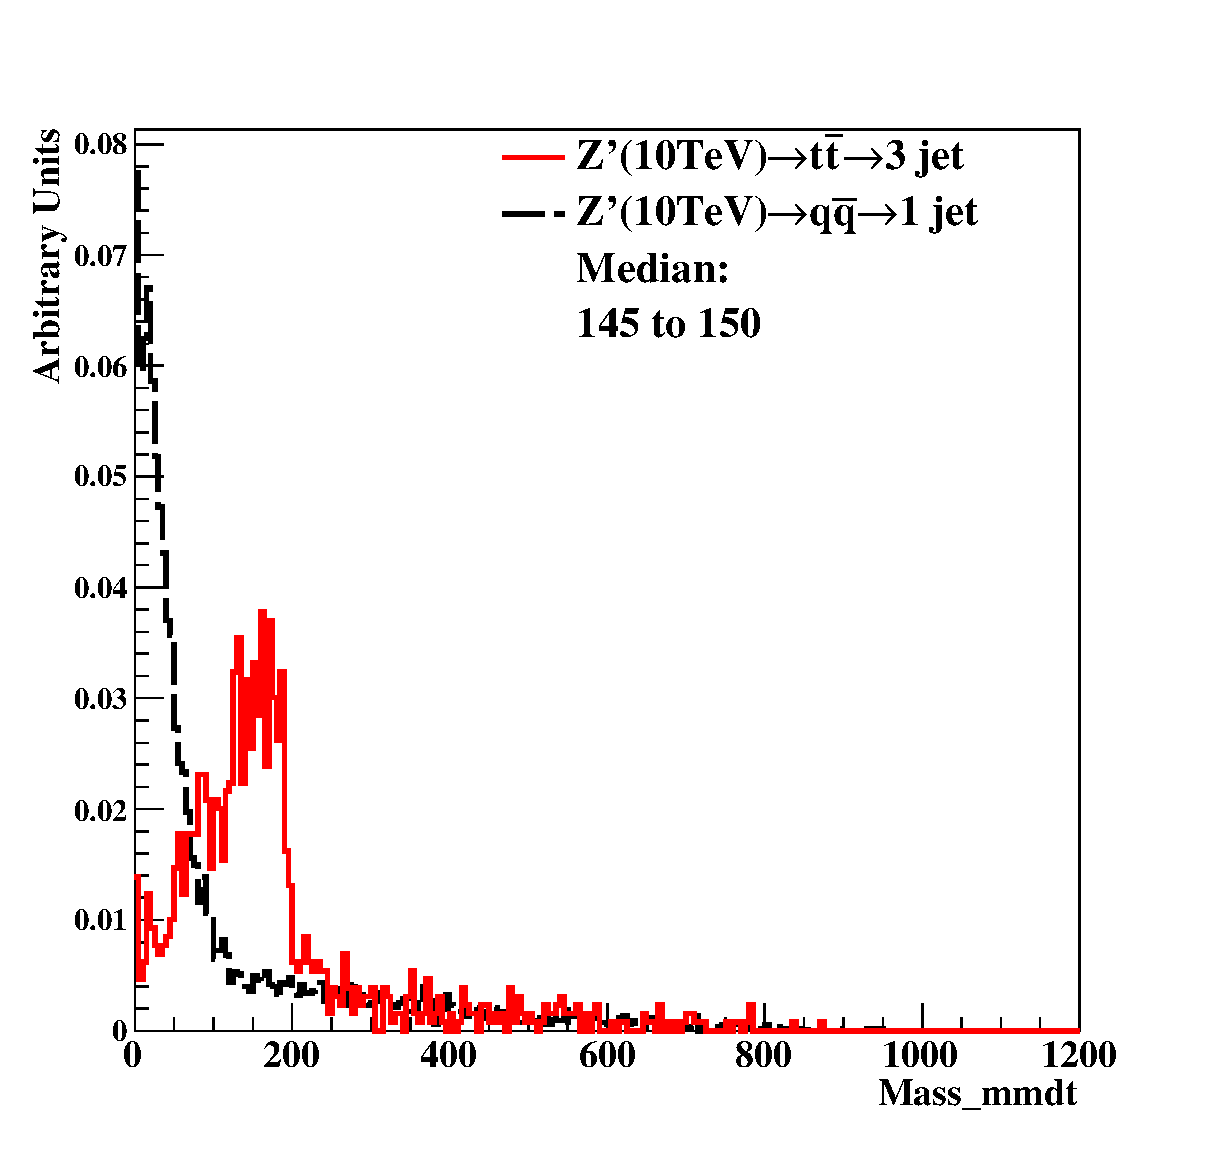
\includegraphics[width=0.22\textwidth]{figs/Dis_cluster_012_mass_mmdt_tt_10tev_04_tt_no_UOF.eps}
   }
   \subfigure[20~TeV at 1$\times$1 (cm$\times$cm) with cluster] {
   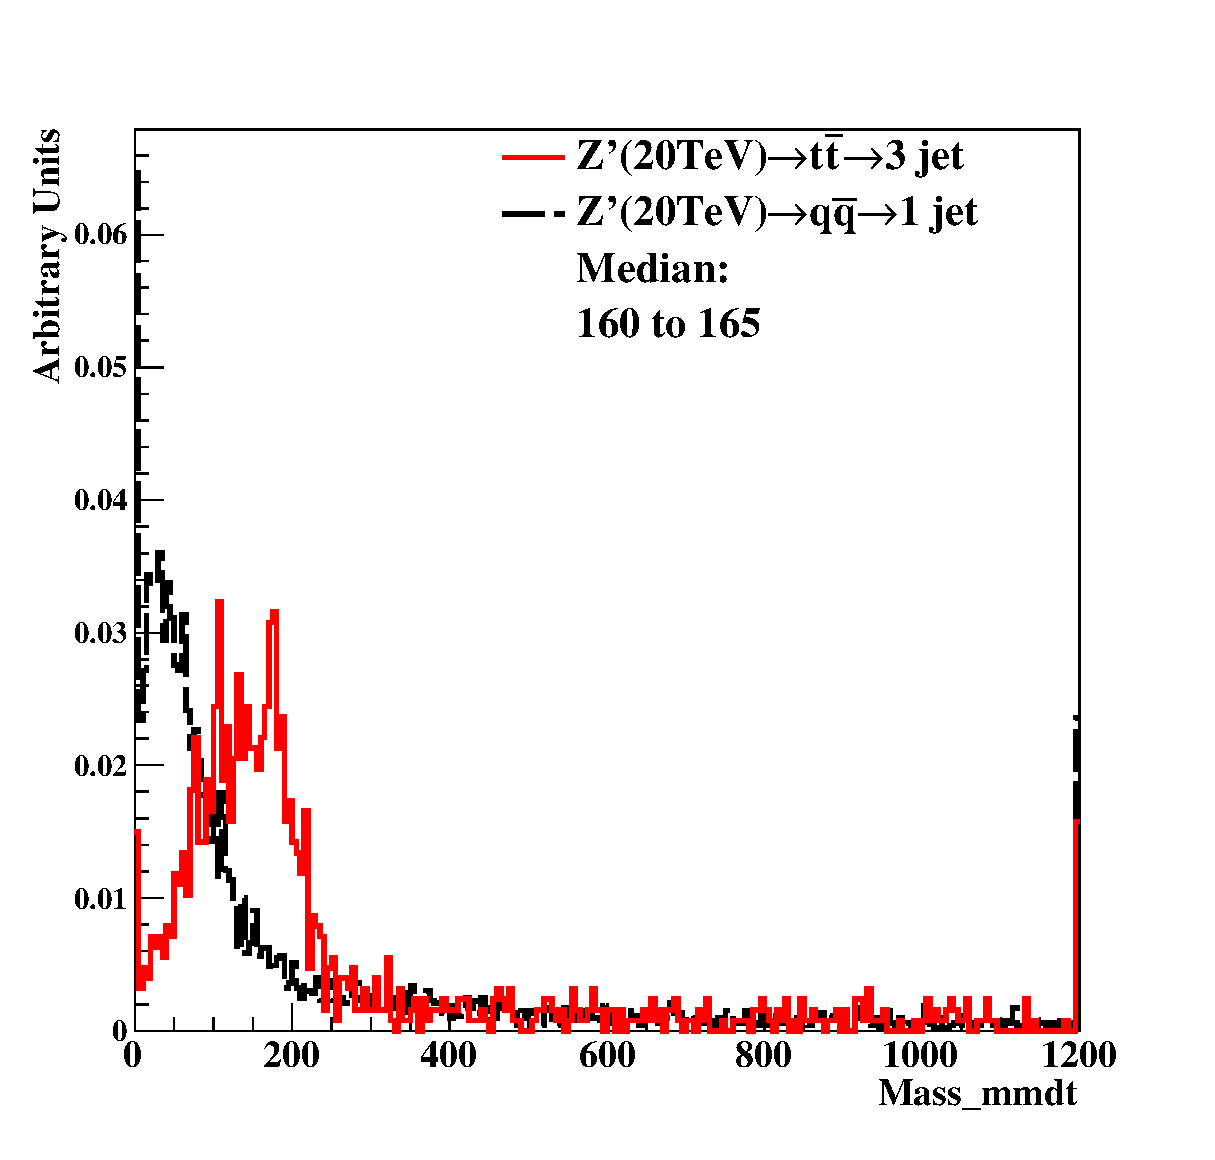
\includegraphics[width=0.22\textwidth]{figs/Dis_cluster_012_mass_mmdt_tt_20tev_04_tt_no_UOF.eps}\hfill
   }
      \subfigure[40~TeV at 1$\times$1 (cm$\times$cm) with cluster] {
   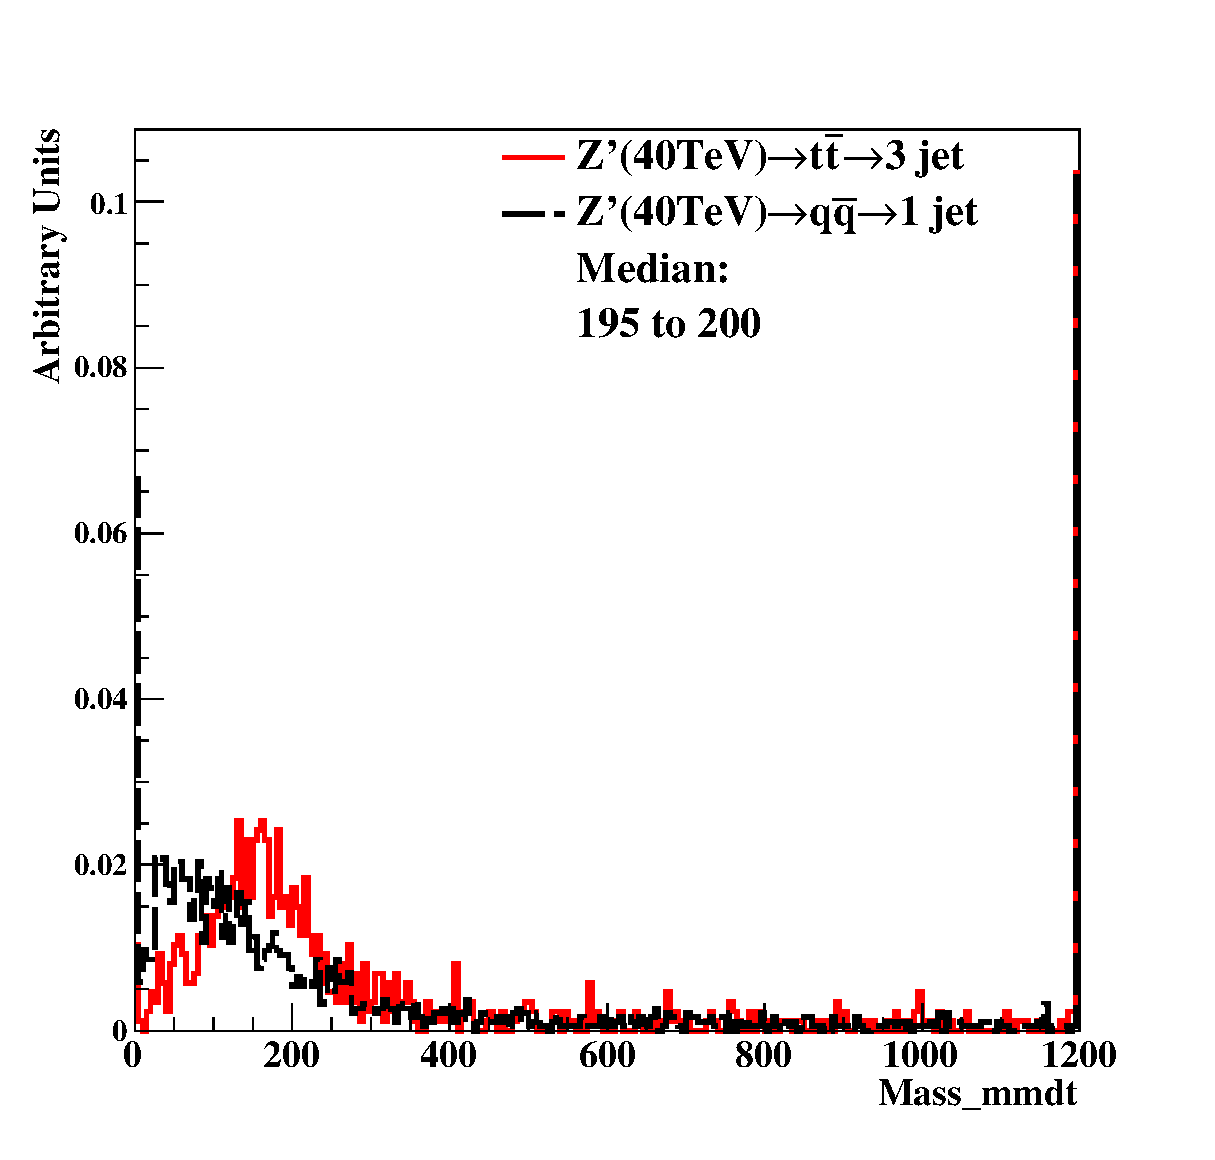
\includegraphics[width=0.22\textwidth]{figs/Dis_cluster_012_mass_mmdt_tt_40tev_04_tt_no_UOF.eps}
   }
\end{center}
\caption{
Distributions of soft drop mass for $\beta$=0, with 5, 10, 20, and 
40~TeV c.m. energies and three different detector cell sizes: 20$\times$20, 
5$\times$5, and 1$\times$1 (cm$\times$cm). The signal (background) process is 
Z'$\rightarrow$t$\bar{\mathrm{t}}$ (Z'$\rightarrow$q$\bar{\mathrm{q}}$).
}
\label{fig:cluster_mass_mmdt_tt}
\end{figure}


\begin{figure}
\begin{center}
  \subfigure[Central at Median($20\times20$=,$5\times5$=,$1\times1$=) change width with cluster at 5~TeV] {
  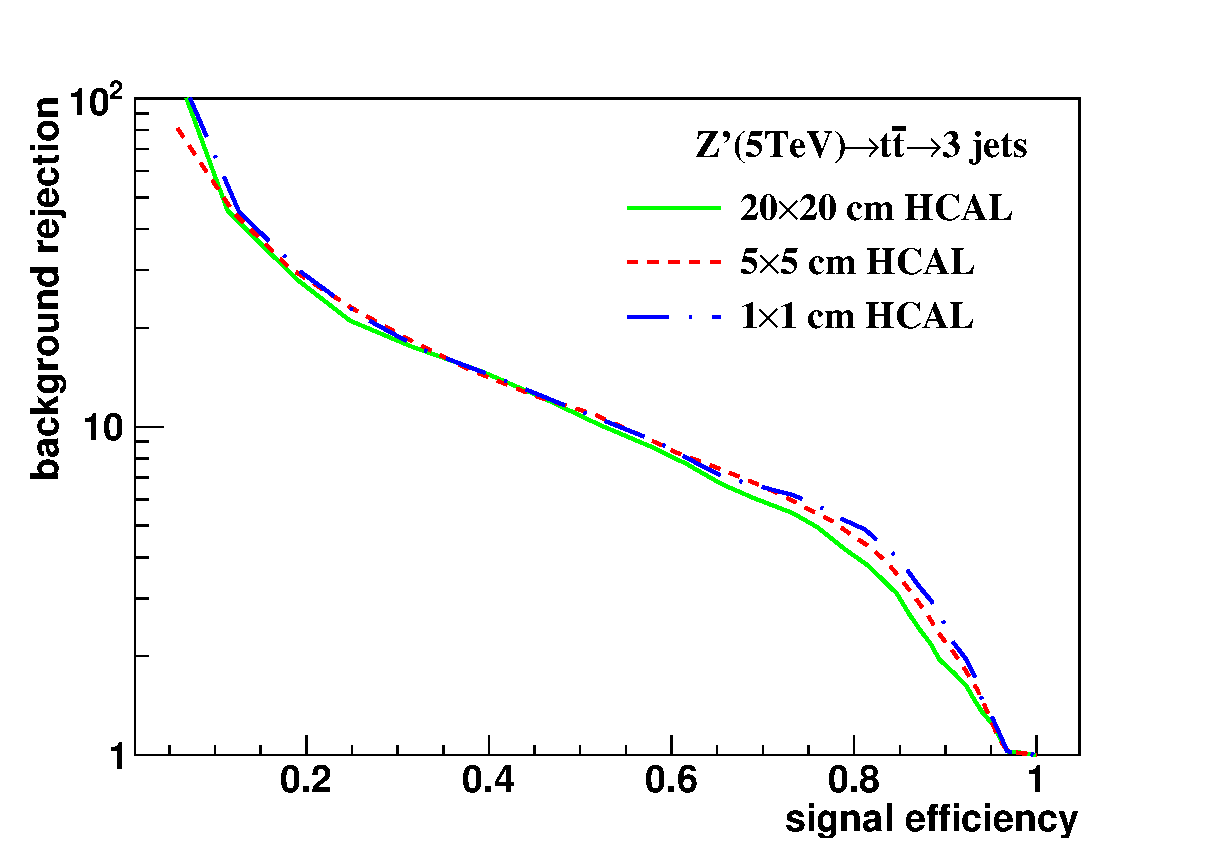
\includegraphics[width=0.43\textwidth]{figs/A_Cluster_mass_mmdt_5tev_eff_1_central_fix_at_Median_bin_tt_qq_log_no_UOF.eps}
  }
  \subfigure[Central at Median($20\times20$=,$5\times5$=,$1\times1$=) change width with cluster at 10~TeV] {
  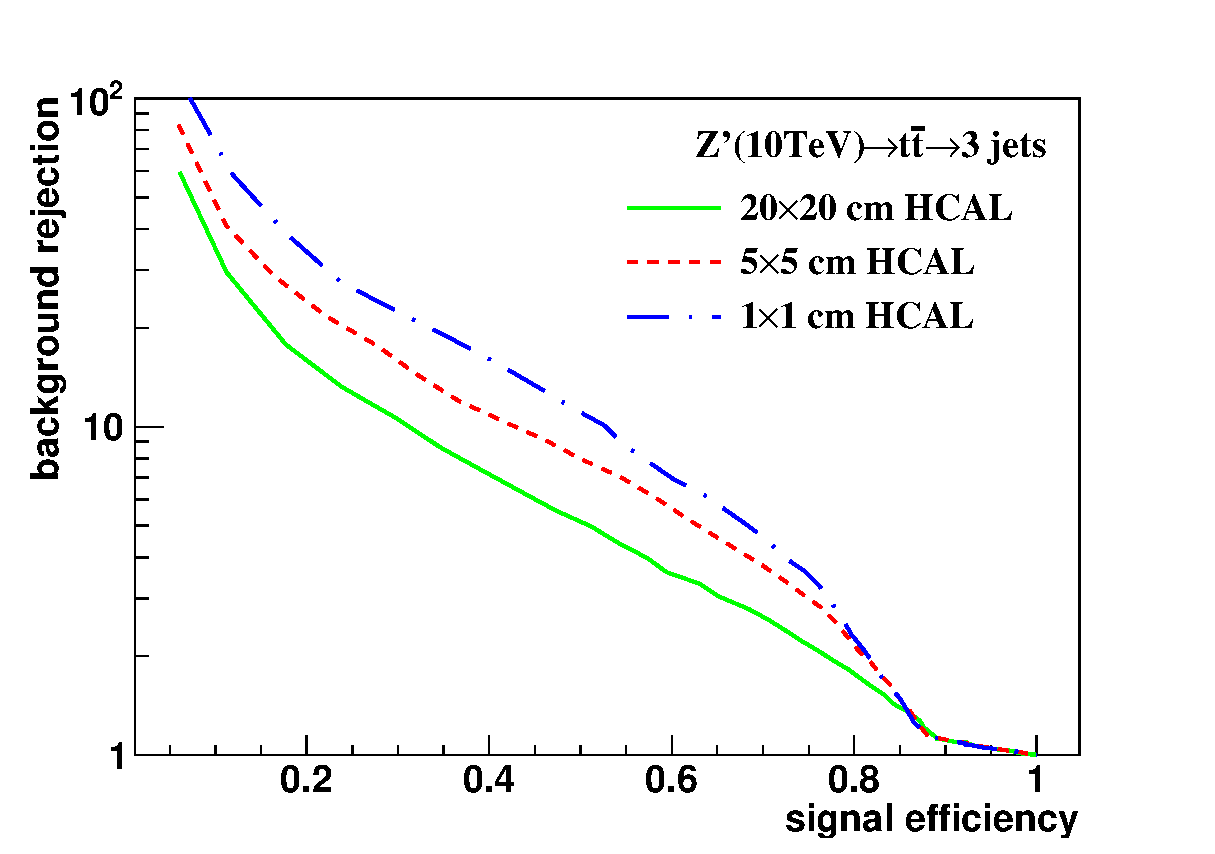
\includegraphics[width=0.43\textwidth]{figs/A_Cluster_mass_mmdt_10tev_eff_1_central_fix_at_Median_bin_tt_qq_log_no_UOF.eps}
  }
 \subfigure[Central at Median($20\times20$=,$5\times5$=,$1\times1$=) change width with cluster at 20~TeV] {
 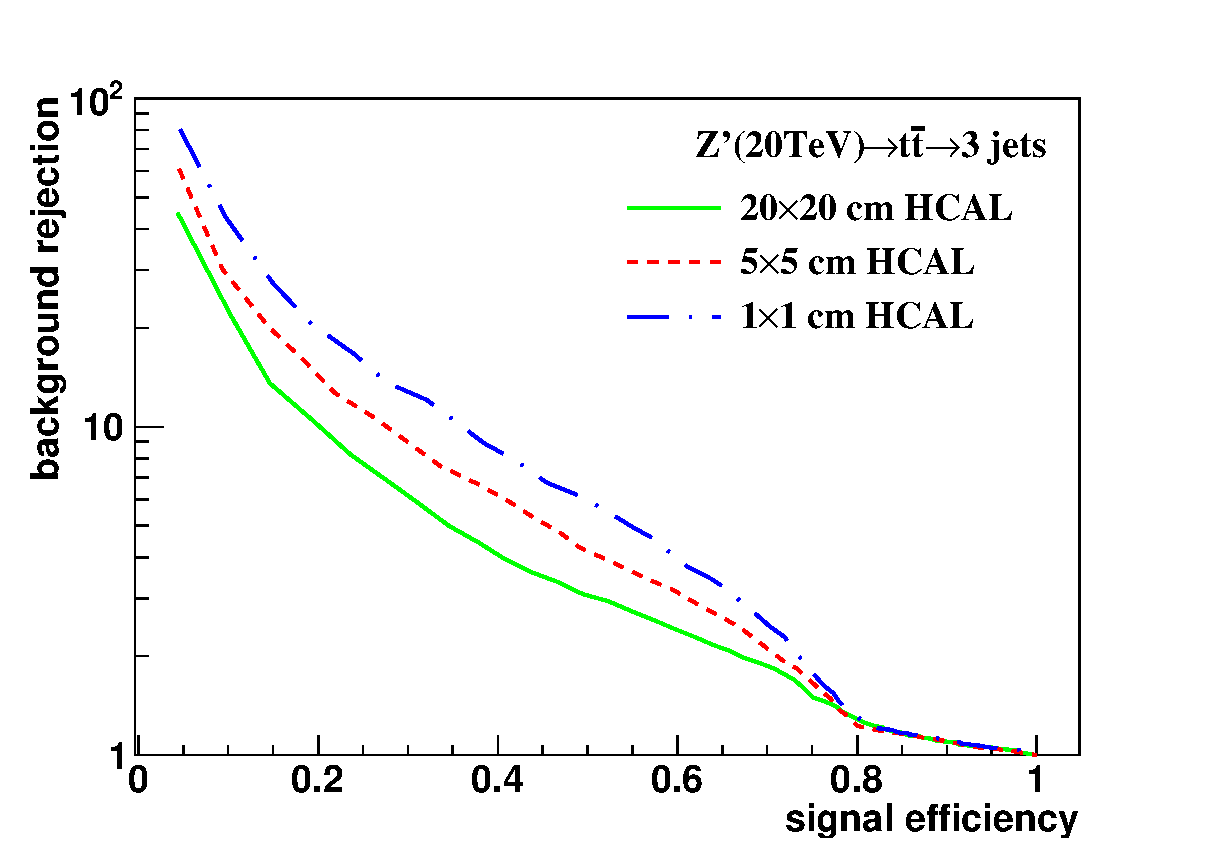
\includegraphics[width=0.43\textwidth]{figs/A_Cluster_mass_mmdt_20tev_eff_1_central_fix_at_Median_bin_tt_qq_log_no_UOF.eps}
 }
 \subfigure[Central at Median($20\times20$=,$5\times5$=,$1\times1$=) change width with cluster at 40~TeV] {
 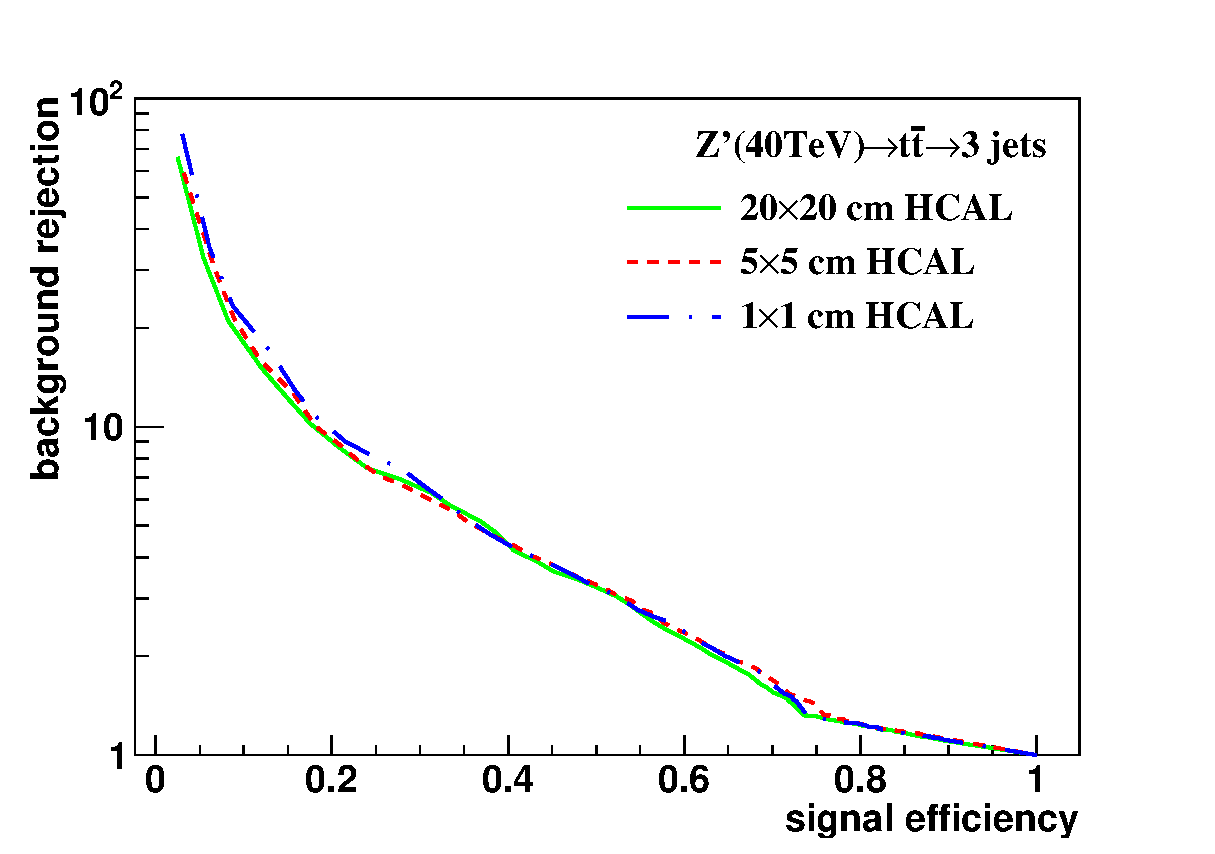
\includegraphics[width=0.43\textwidth]{figs/A_Cluster_mass_mmdt_40tev_eff_1_central_fix_at_Median_bin_tt_qq_log_no_UOF.eps}
 }
\end{center}
\caption{
The ROC curves of soft drop mass selection for $\beta$=0 
with 5, 10, 20, and 40~TeV c.m. energies. 
Three different detector cell sizes are compared: 20$\times$20, 
5$\times$5, and 1$\times$1 (cm$\times$cm). 
The signal (background) process is Z'$\rightarrow$t$\bar{\mathrm{t}}$
(Z'$\rightarrow$q$\bar{\mathrm{q}}$).
}
\label{fig:cluster_mass_mmdt_tt_ROC}
\end{figure}



\begin{figure}
\begin{center}
   \subfigure[5~TeV at 20$\times$20 (cm$\times$cm) with cluster] {
   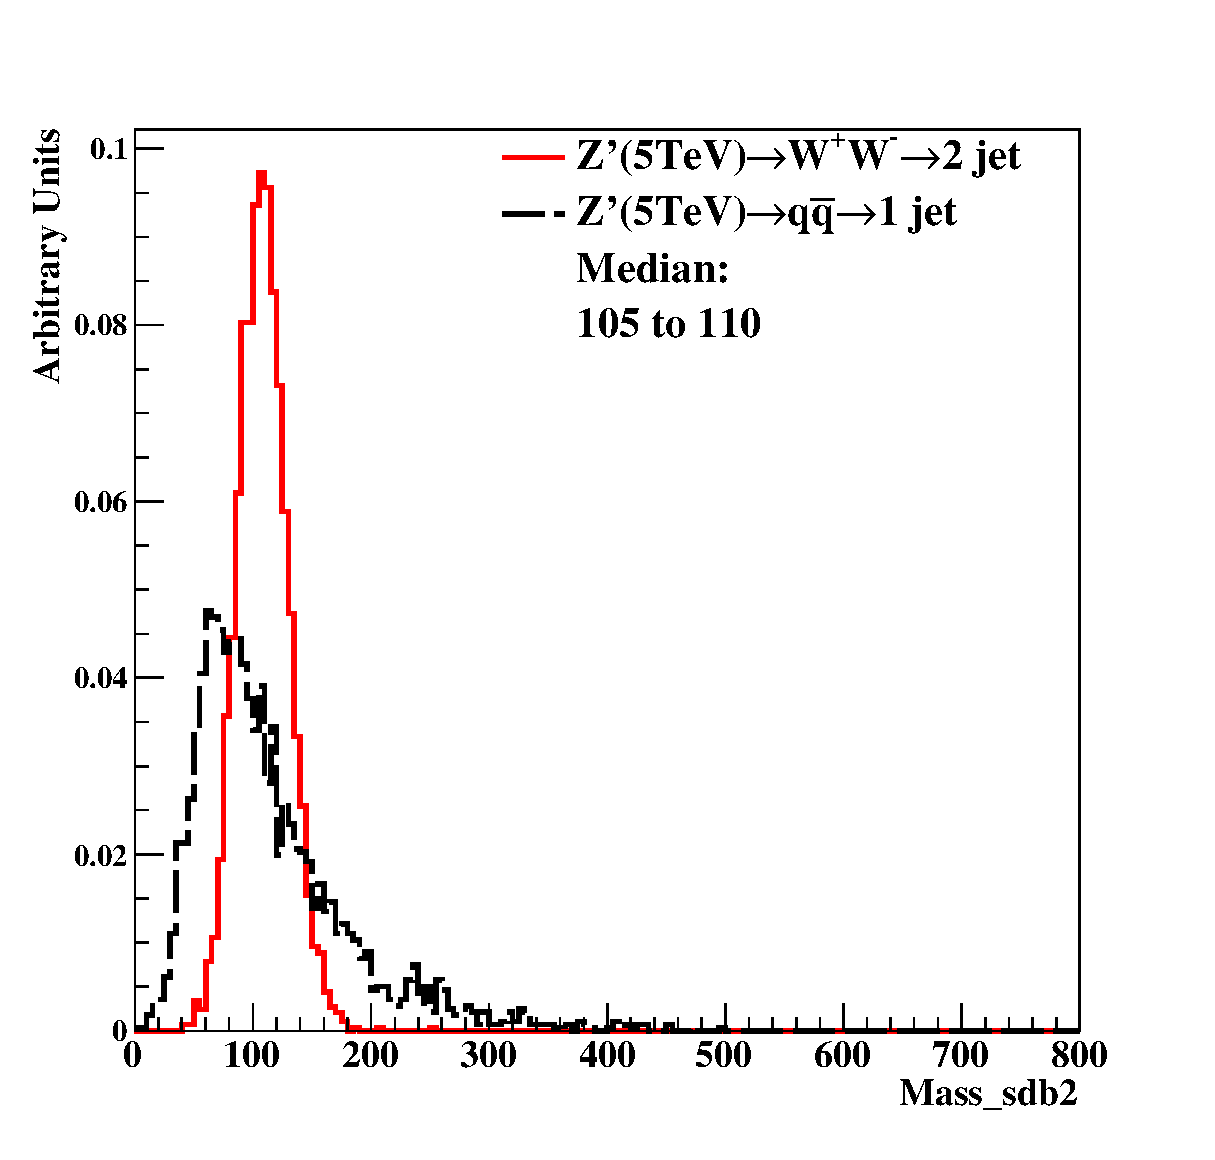
\includegraphics[width=0.22\textwidth]{figs/Dis_cluster_010_mass_sdb2_ww_5tev_04_800_no_UOF.eps}
   }
      \subfigure[10~TeV at 20$\times$20 (cm$\times$cm) with cluster] {
   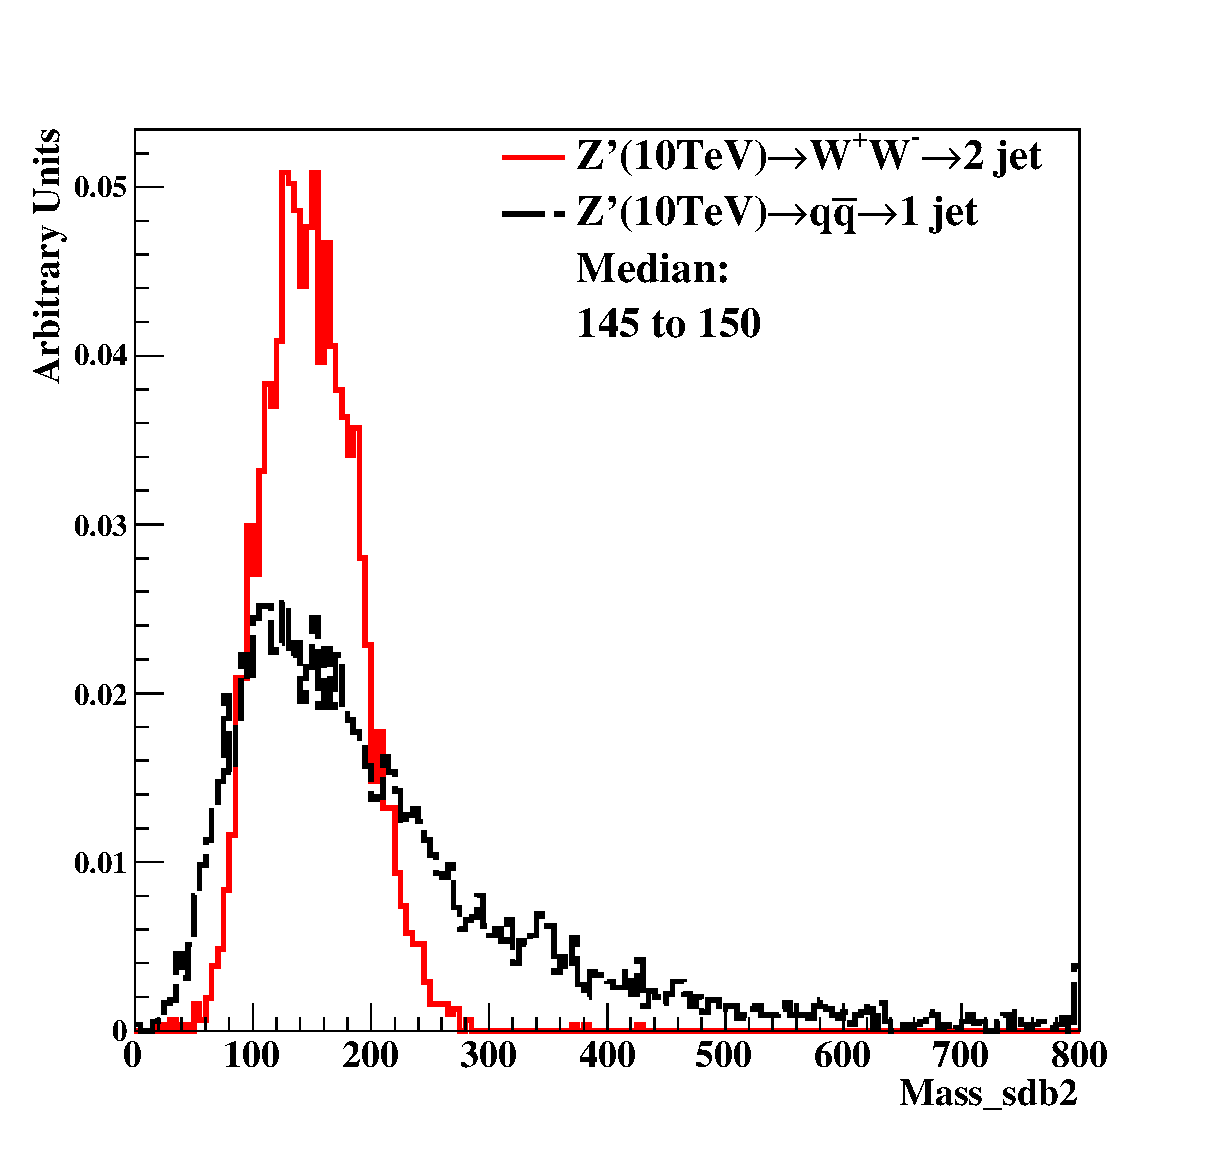
\includegraphics[width=0.22\textwidth]{figs/Dis_cluster_010_mass_sdb2_ww_10tev_04_800_no_UOF.eps}
   }
   \subfigure[20~TeV at 20$\times$20 (cm$\times$cm) with cluster] {
   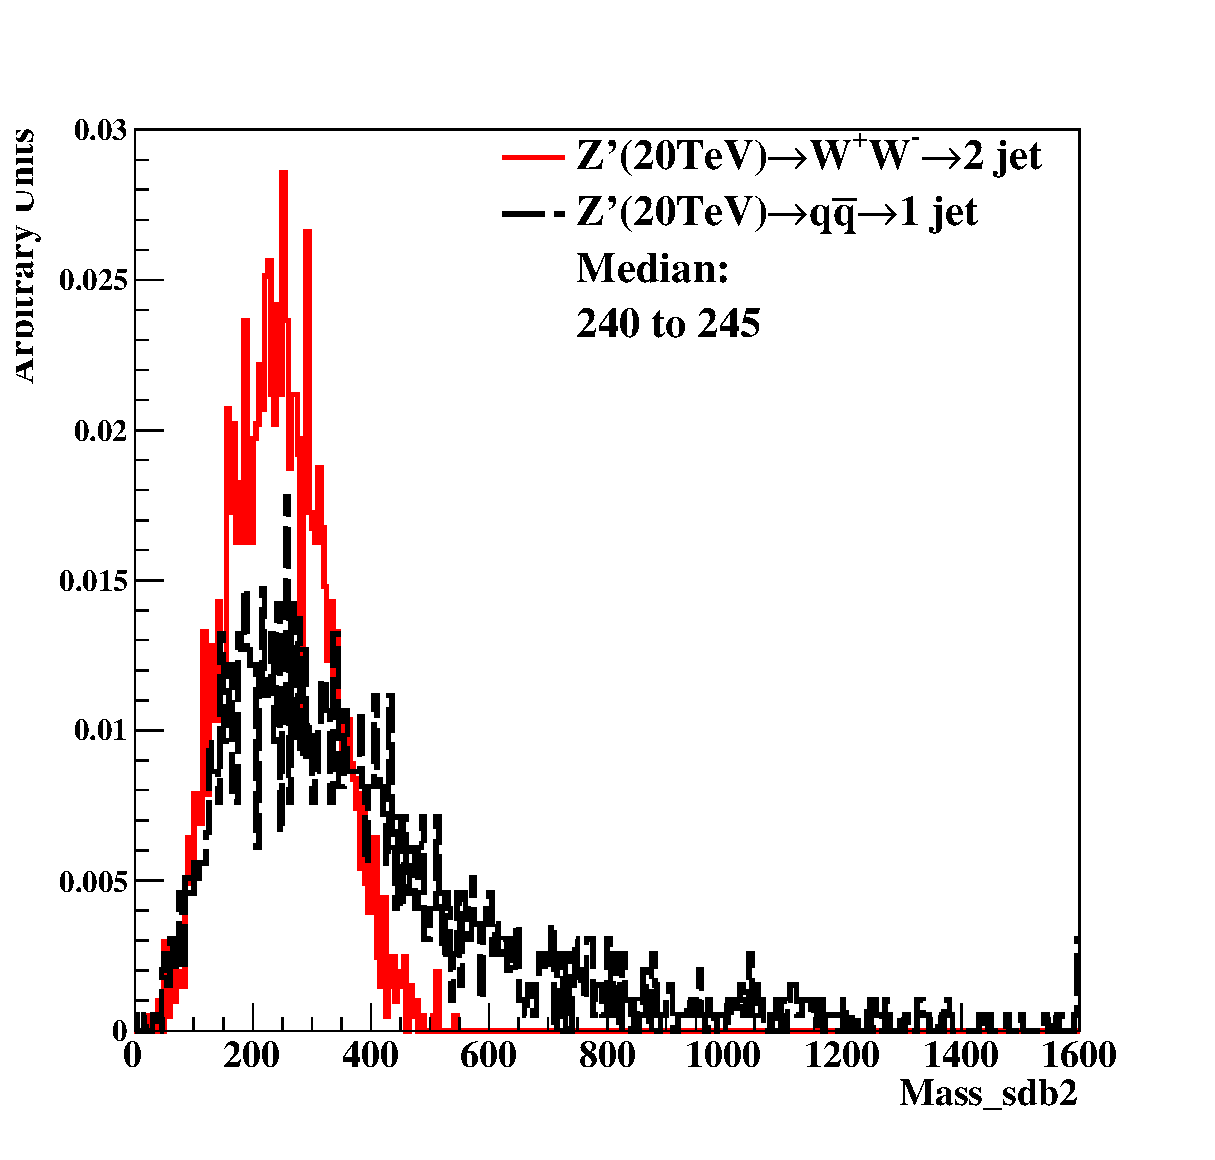
\includegraphics[width=0.22\textwidth]{figs/Dis_cluster_010_mass_sdb2_ww_20tev_04_1600_no_UOF.eps}
   }
    \subfigure[40~TeV at 20$\times$20 (cm$\times$cm) with cluster] {
   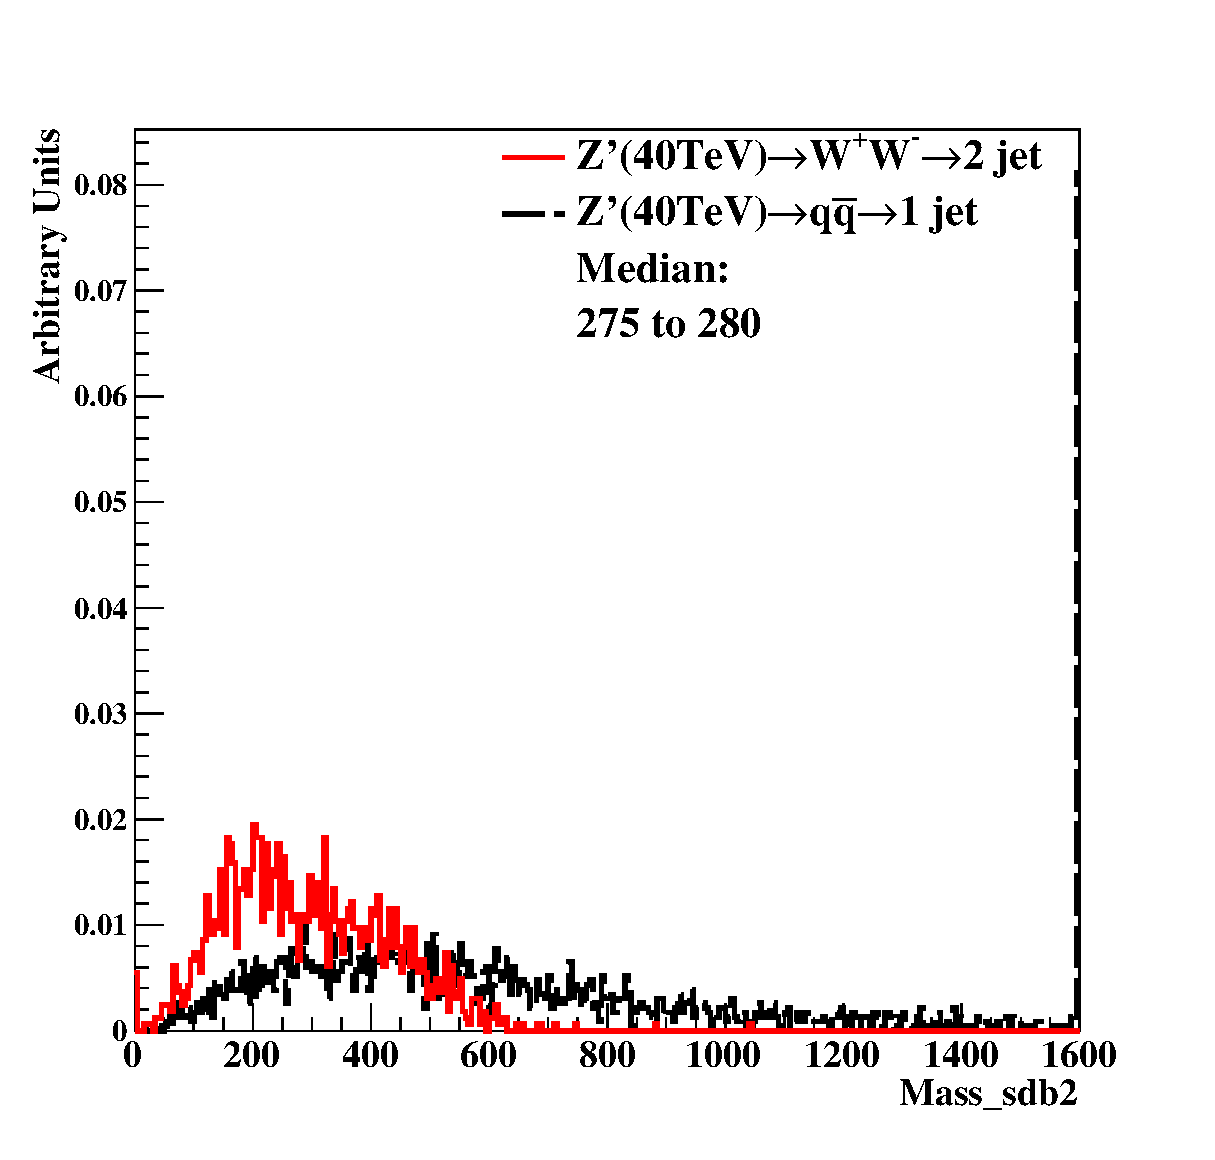
\includegraphics[width=0.22\textwidth]{figs/Dis_cluster_010_mass_sdb2_ww_40tev_04_1600_no_UOF.eps}
   }
   \subfigure[5~TeV at 5$\times$5 (cm$\times$cm) with cluster] {
   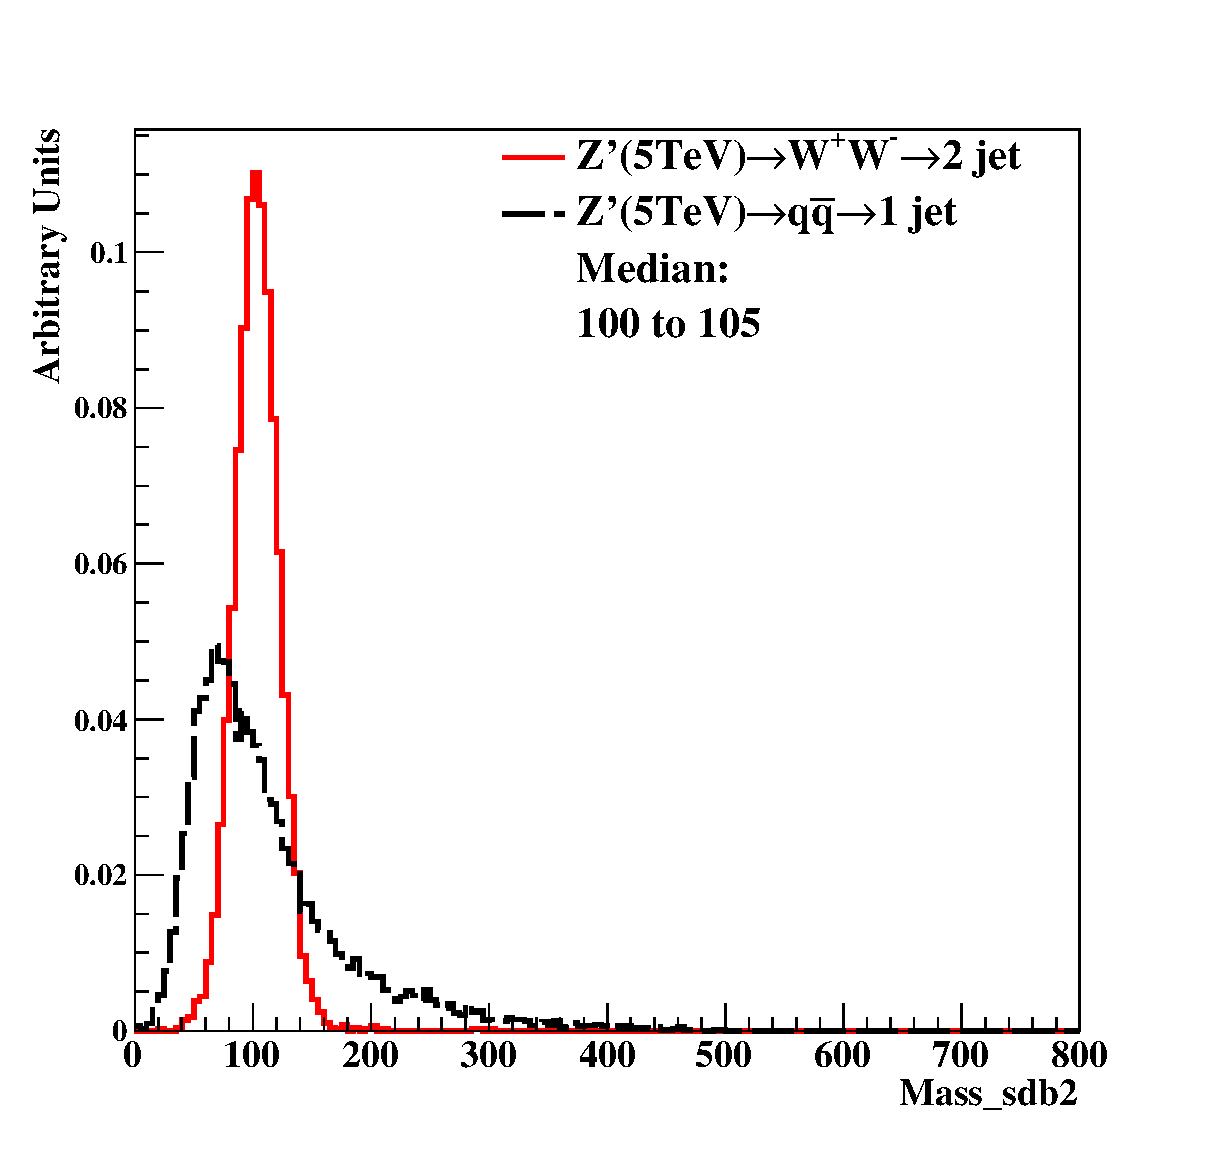
\includegraphics[width=0.22\textwidth]{figs/Dis_cluster_009_mass_sdb2_ww_5tev_04_800_no_UOF.eps}
   }
   \subfigure[10~TeV at 5$\times$5 (cm$\times$cm) with cluster] {
   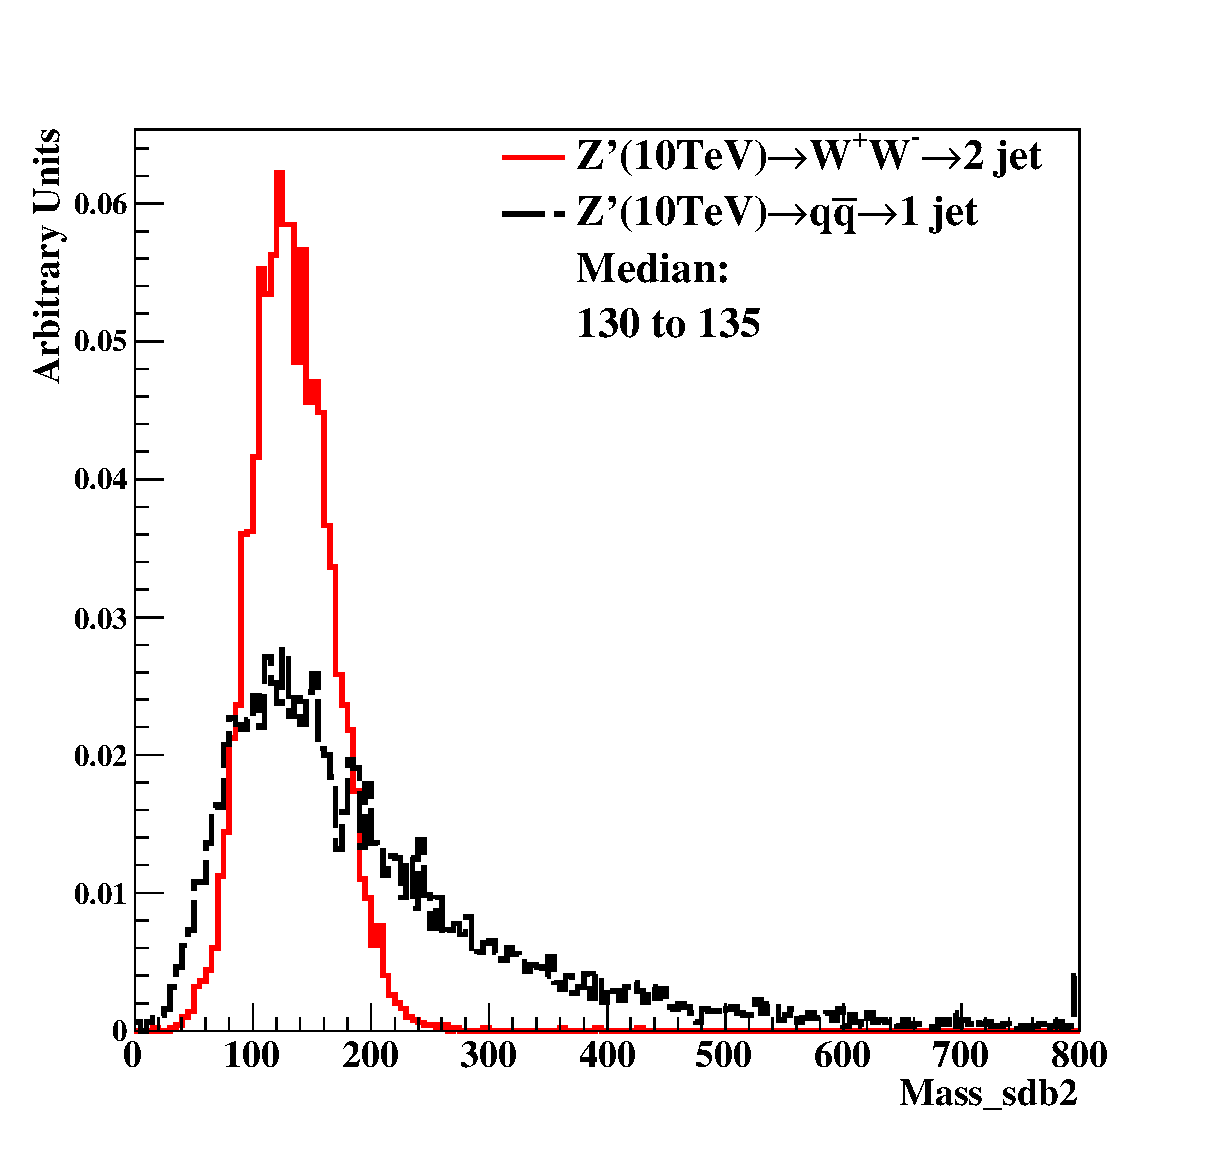
\includegraphics[width=0.22\textwidth]{figs/Dis_cluster_009_mass_sdb2_ww_10tev_04_800_no_UOF.eps}
   }
    \subfigure[20~TeV at 5$\times$5 (cm$\times$cm) with cluster] {
   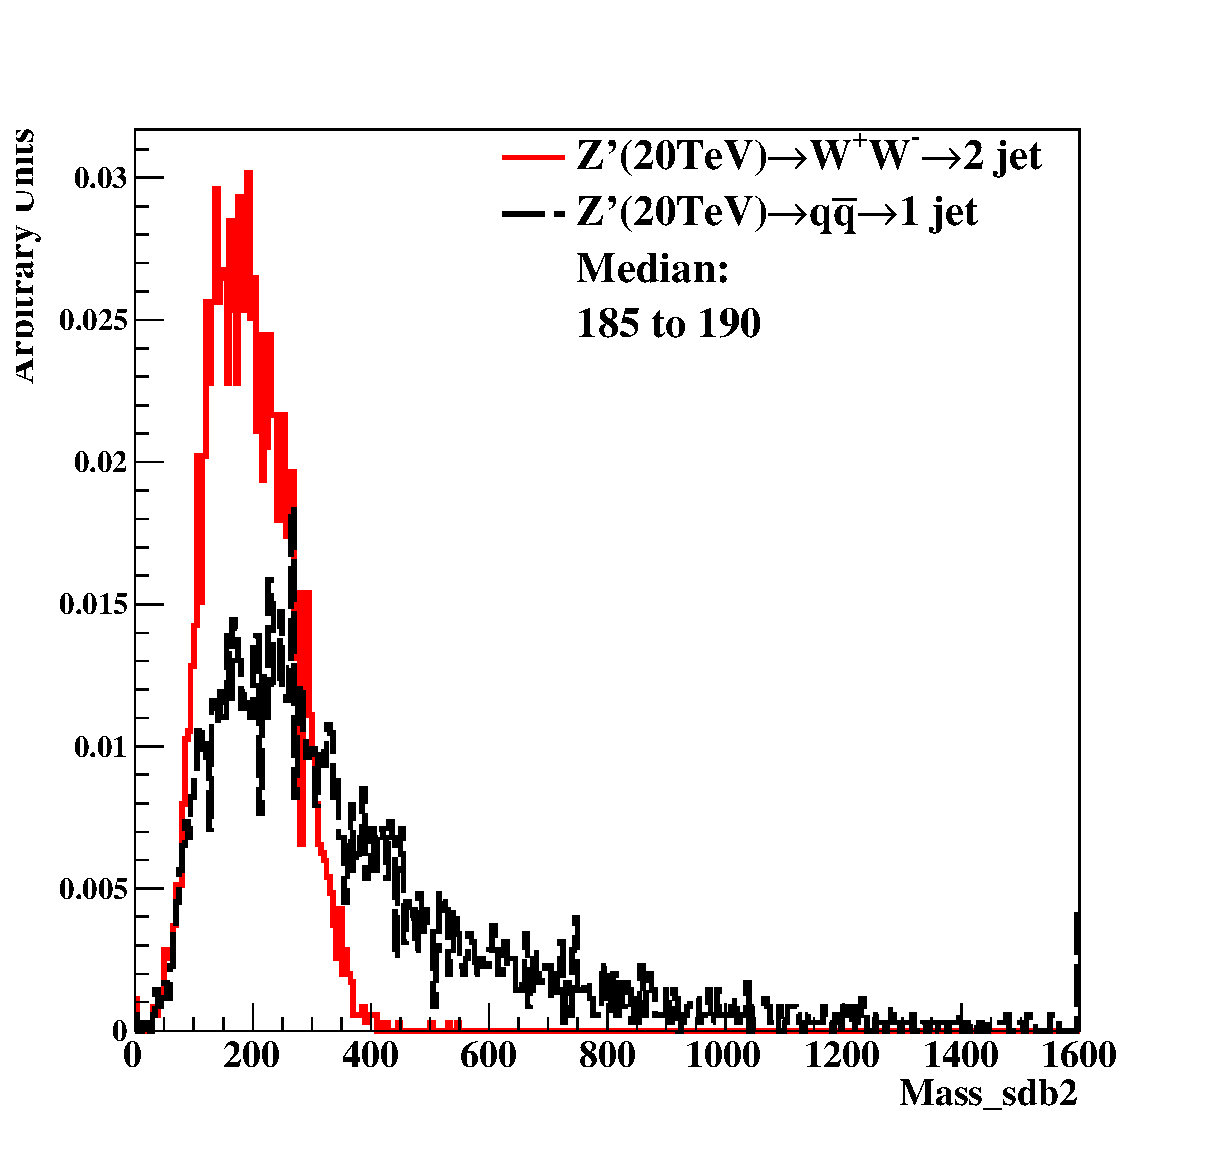
\includegraphics[width=0.22\textwidth]{figs/Dis_cluster_009_mass_sdb2_ww_20tev_04_1600_no_UOF.eps}\hfill
   }
      \subfigure[40~TeV at 5$\times$5 (cm$\times$cm) with cluster] {
   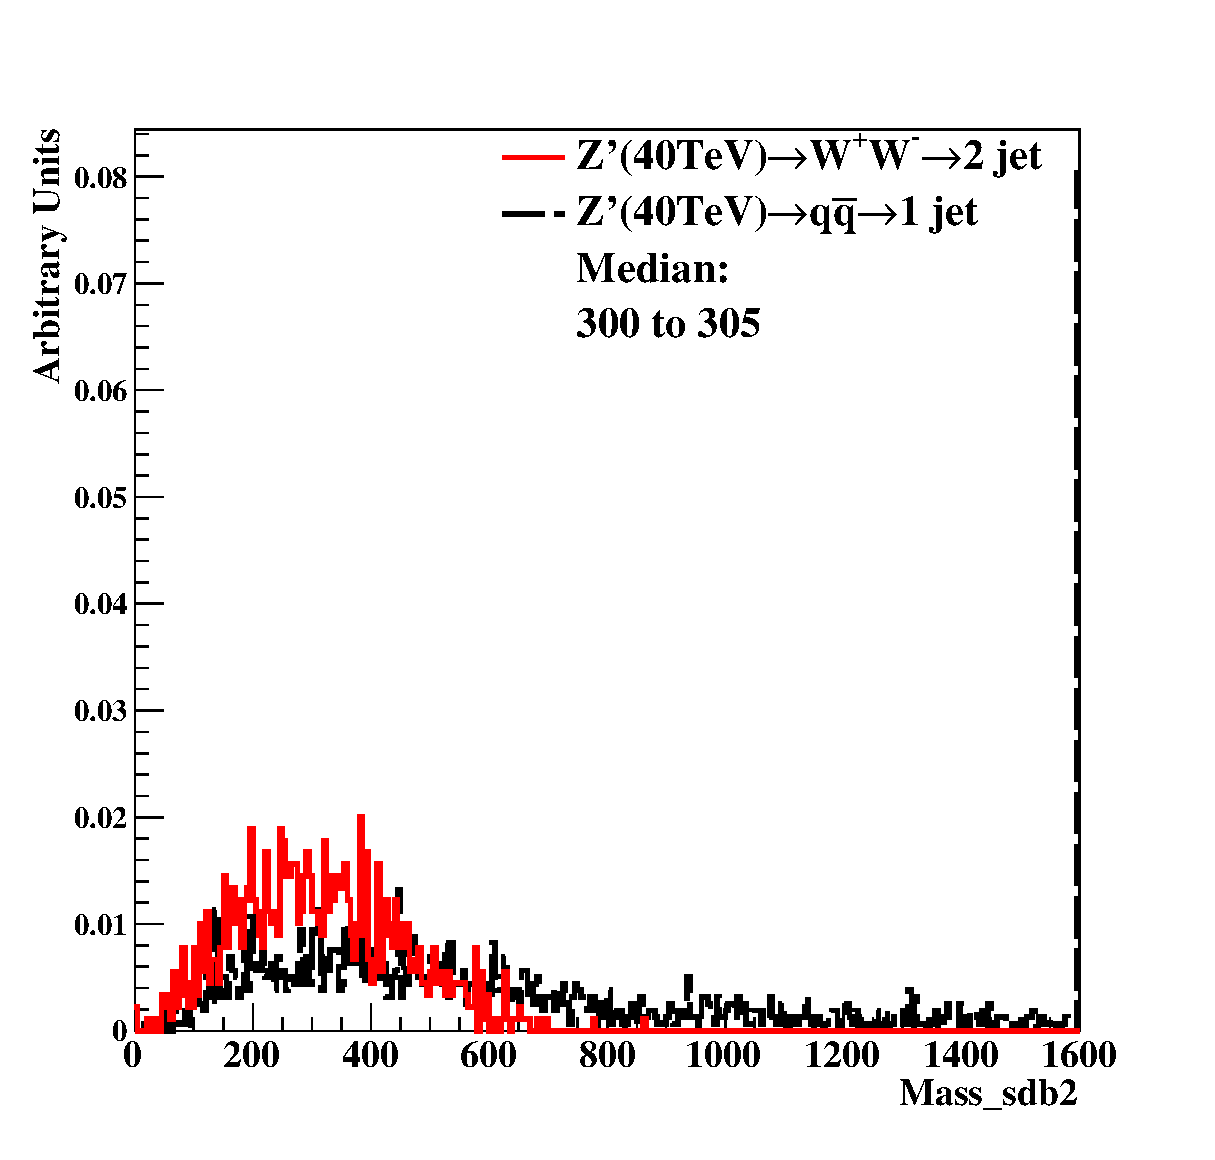
\includegraphics[width=0.22\textwidth]{figs/Dis_cluster_009_mass_sdb2_ww_40tev_04_1600_no_UOF.eps}\hfill
   }
   \subfigure[5~TeV at 1$\times$1 (cm$\times$cm) with cluster] {
   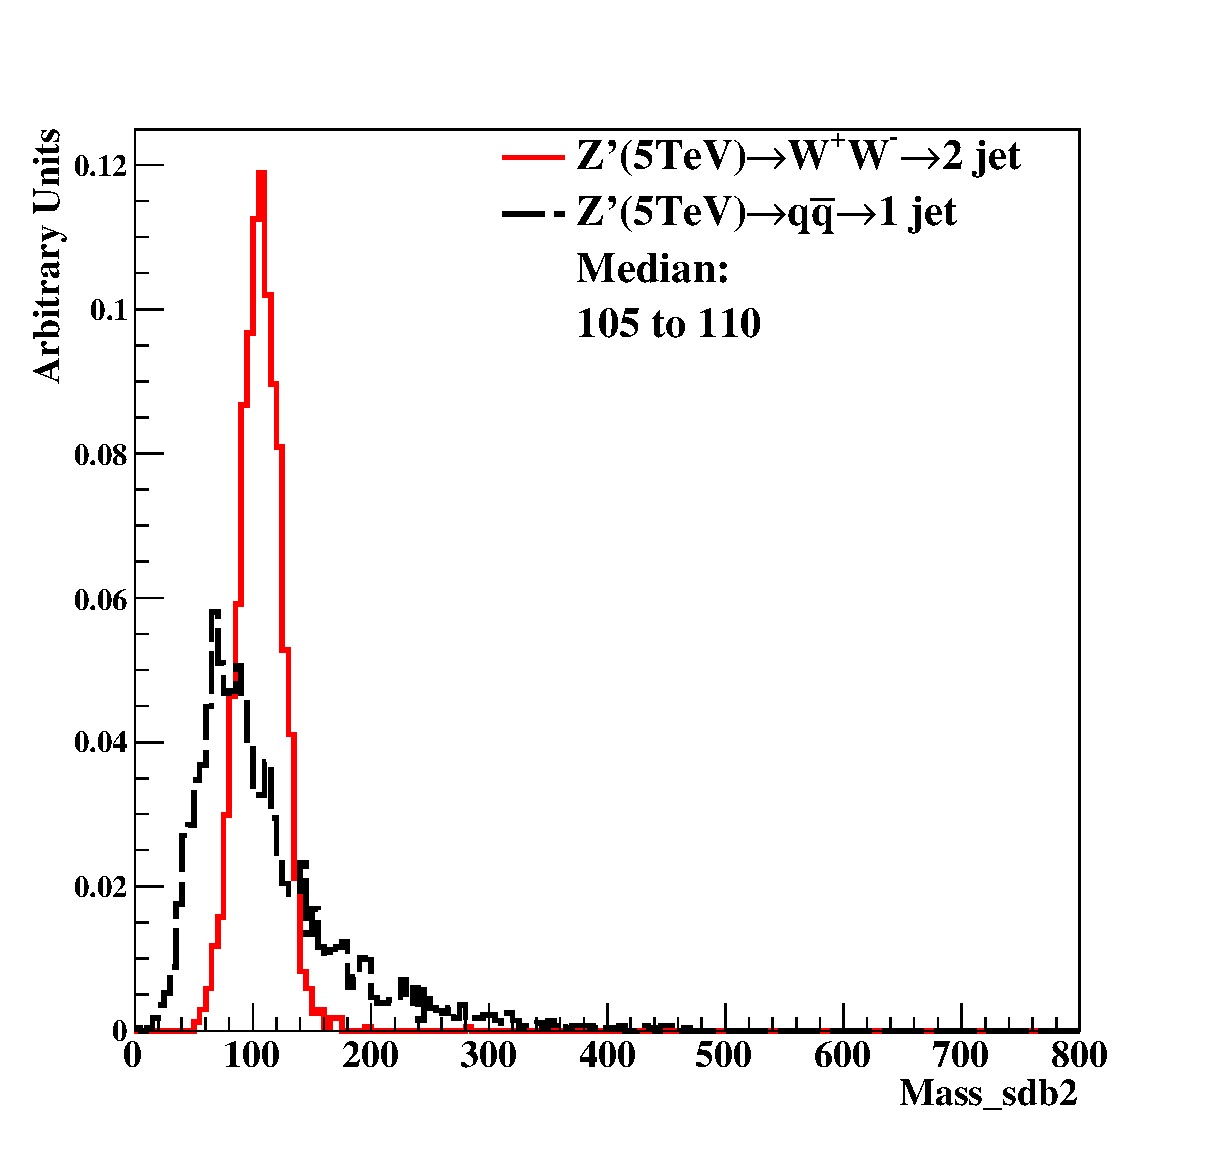
\includegraphics[width=0.22\textwidth]{figs/Dis_cluster_012_mass_sdb2_ww_5tev_04_800_no_UOF.eps}\hfill
   }
    \subfigure[10~TeV at 1$\times$1 (cm$\times$cm) with cluster] {
   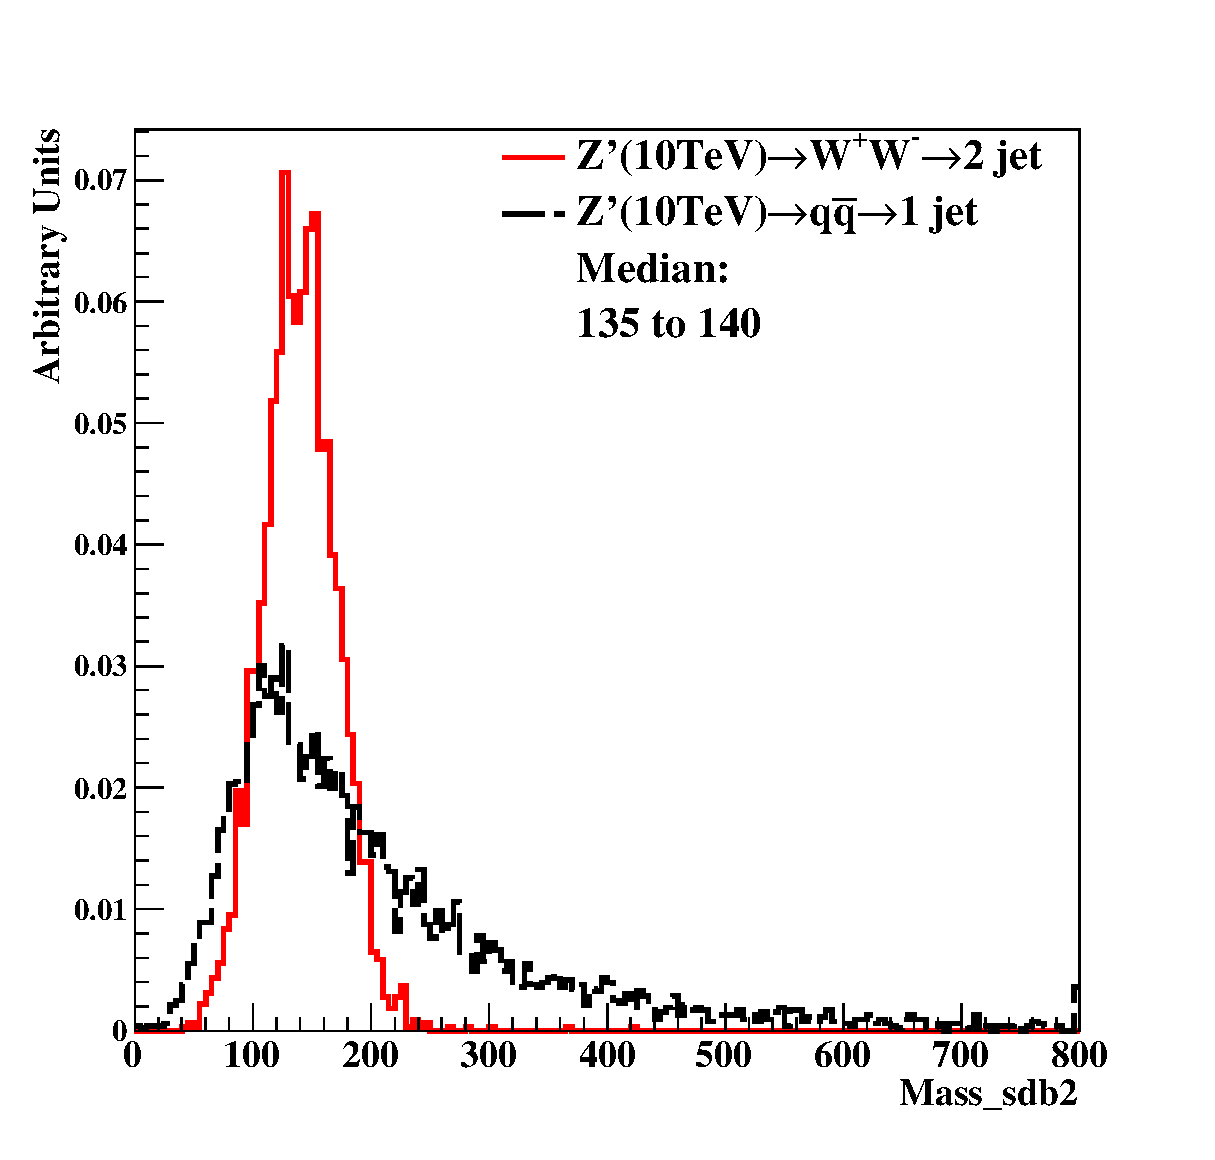
\includegraphics[width=0.22\textwidth]{figs/Dis_cluster_012_mass_sdb2_ww_10tev_04_800_no_UOF.eps}
   }
   \subfigure[20~TeV at 1$\times$1 (cm$\times$cm) with cluster] {
   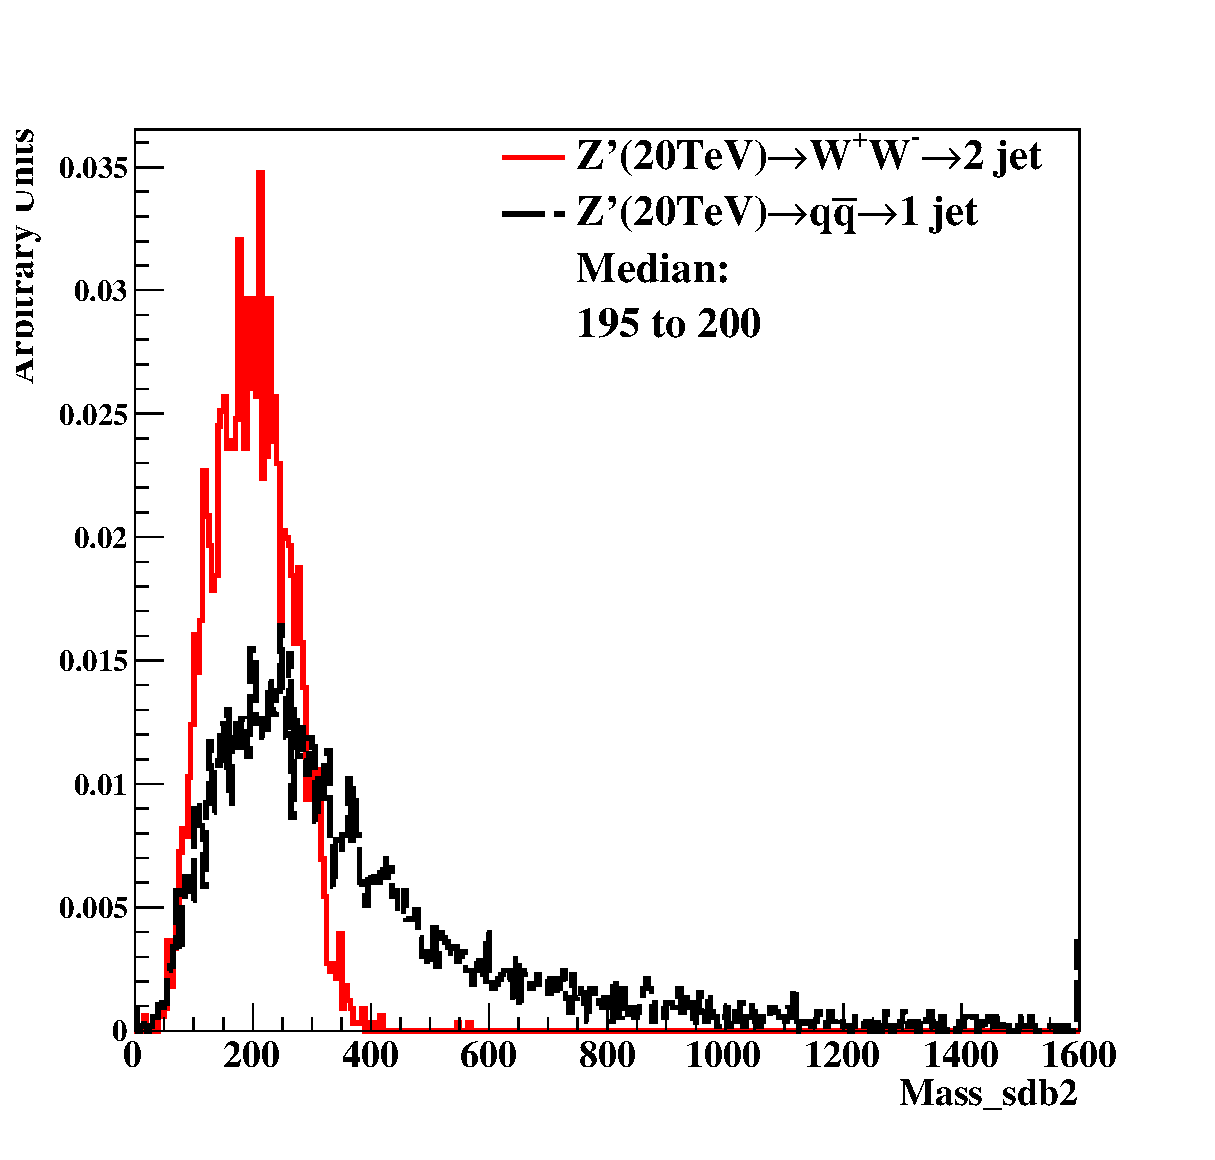
\includegraphics[width=0.22\textwidth]{figs/Dis_cluster_012_mass_sdb2_ww_20tev_04_1600_no_UOF.eps}\hfill
   }
      \subfigure[40~TeV at 1$\times$1 (cm$\times$cm) with cluster] {
   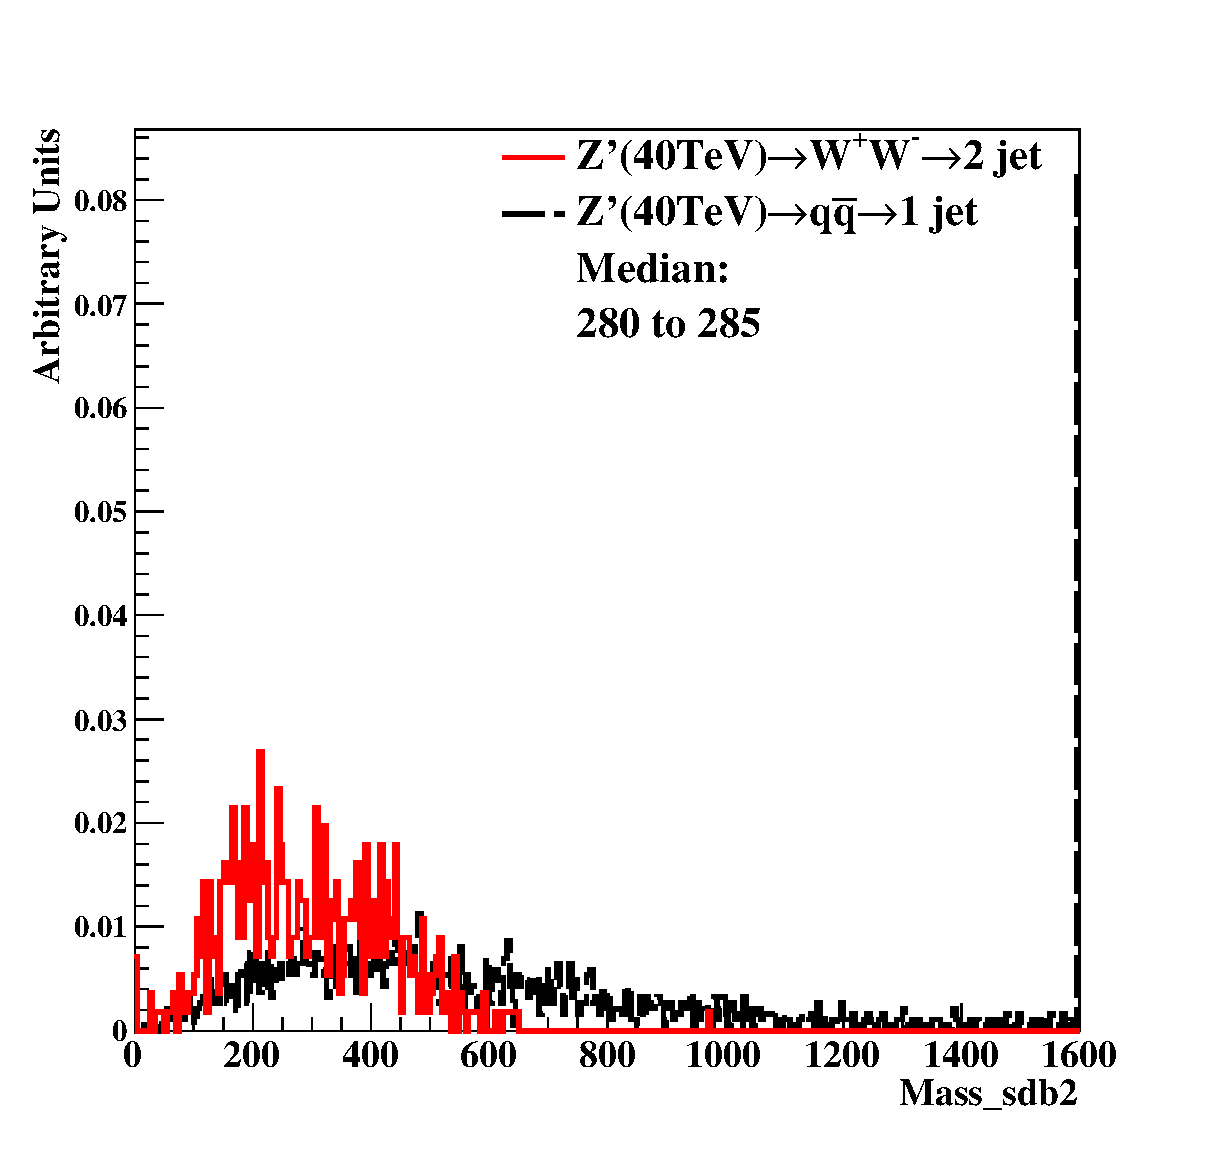
\includegraphics[width=0.22\textwidth]{figs/Dis_cluster_012_mass_sdb2_ww_40tev_04_1600_no_UOF.eps}
   }
\end{center}
\caption{
Distributions of soft drop mass for $\beta$=2, with 5, 10, 20, and 
40~TeV c.m. energies and three different detector cell sizes: 20$\times$20, 
5$\times$5, and 1$\times$1 (cm$\times$cm). The signal (background) process is 
Z'$\rightarrow$WW (Z'$\rightarrow$q$\bar{\mathrm{q}}$).
}
\label{fig:cluster_mass_sdb2_ww}
\end{figure}


\begin{figure}
\begin{center}
  \subfigure[Central at Median($20\times20$=,$5\times5$=,$1\times1$=) change width with cluster at 5~TeV] {
  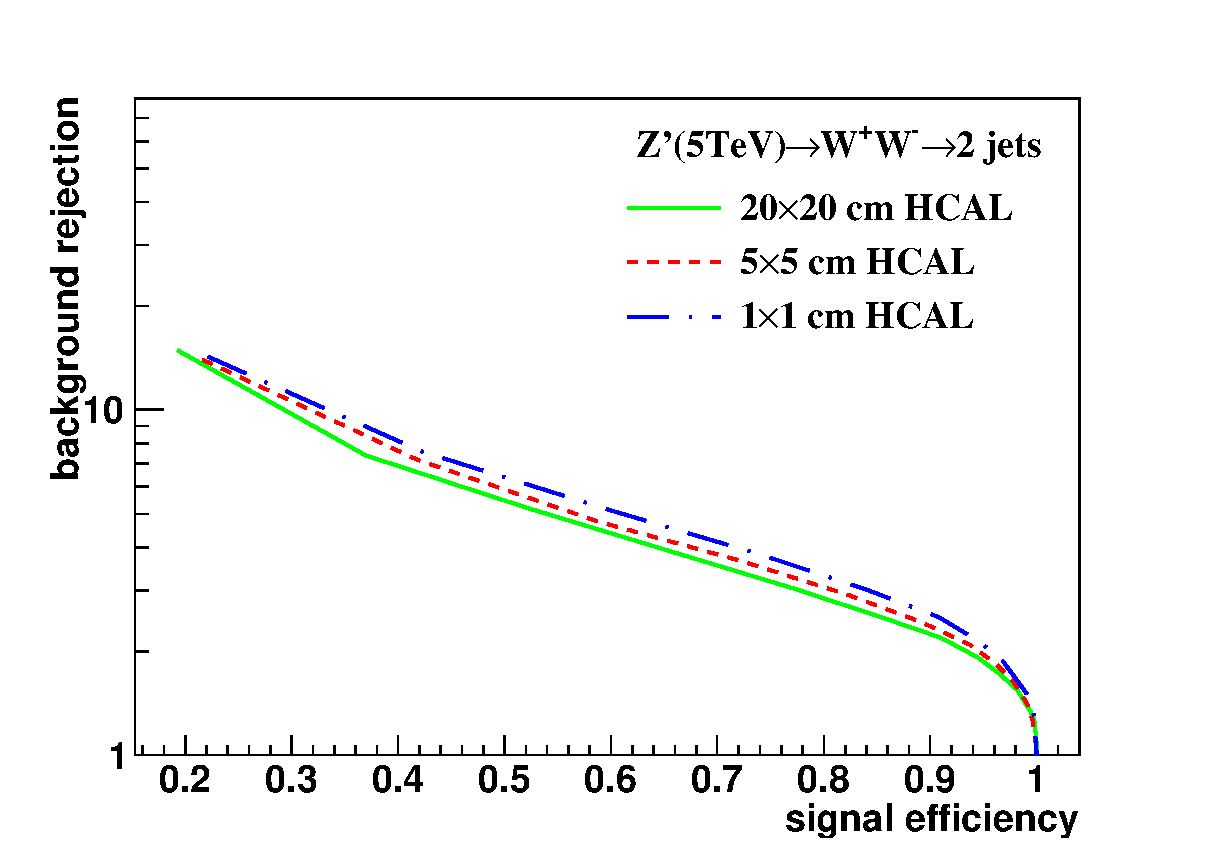
\includegraphics[width=0.43\textwidth]{figs/A_Cluster_mass_sdb2_5tev_eff_1_central_fix_at_Median_bin_ww_qq_log_no_UOF.eps}
  }
  \subfigure[Central at Median($20\times20$=,$5\times5$=,$1\times1$=) change width with cluster at 10~TeV] {
  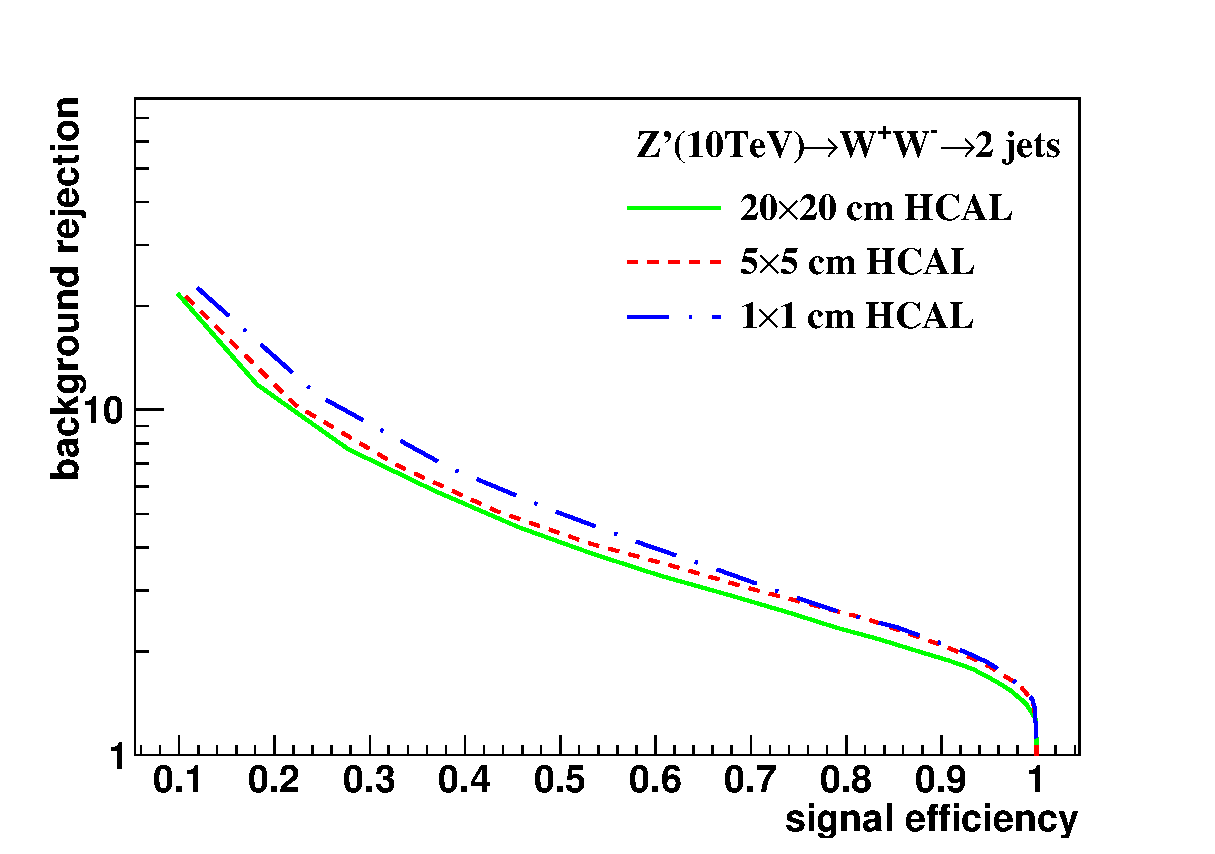
\includegraphics[width=0.43\textwidth]{figs/A_Cluster_mass_sdb2_10tev_eff_1_central_fix_at_Median_bin_ww_qq_log_no_UOF.eps}
  }
 \subfigure[Central at Median($20\times20$=,$5\times5$=,$1\times1$=) change width with cluster at 20~TeV] {
 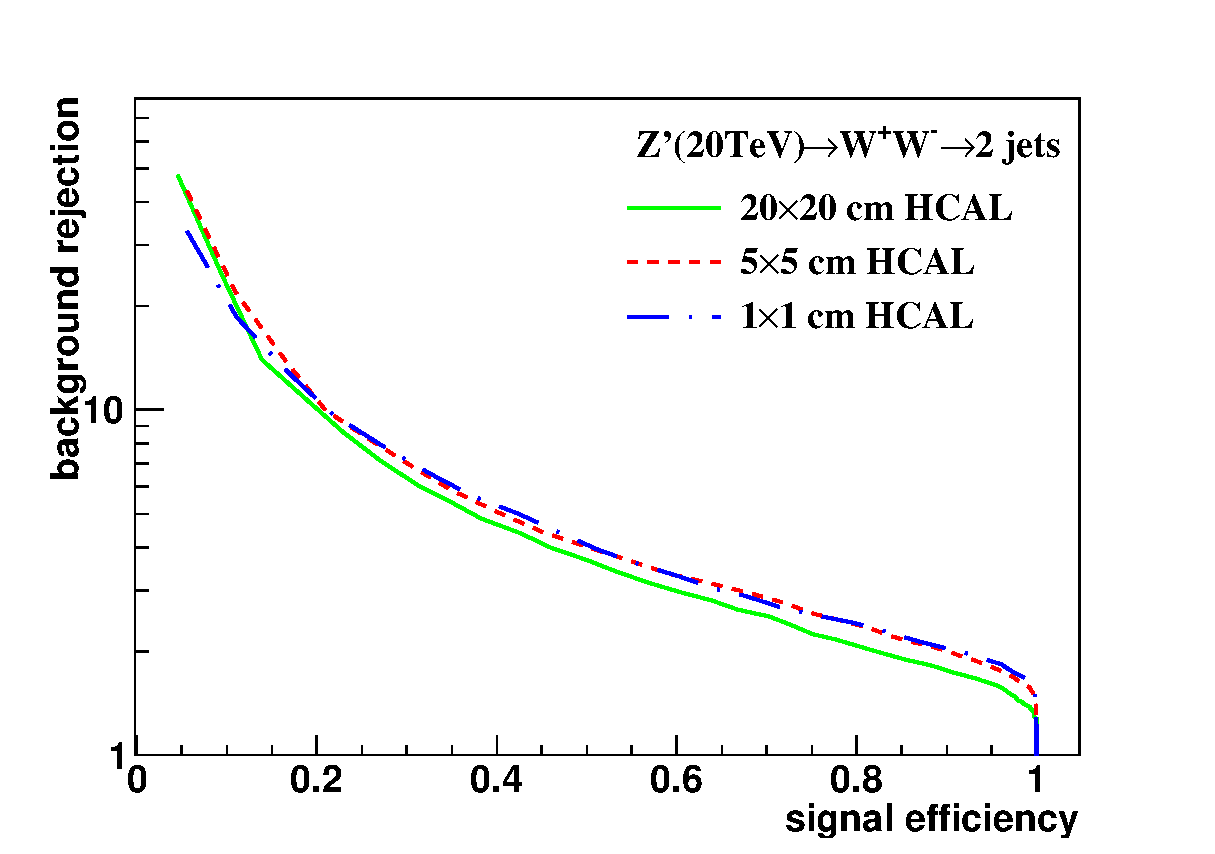
\includegraphics[width=0.43\textwidth]{figs/A_Cluster_mass_sdb2_20tev_eff_1_central_fix_at_Median_bin_ww_qq_log_no_UOF.eps}
 }
 \subfigure[Central at Median($20\times20$=,$5\times5$=,$1\times1$=) change width with cluster at 40~TeV] {
 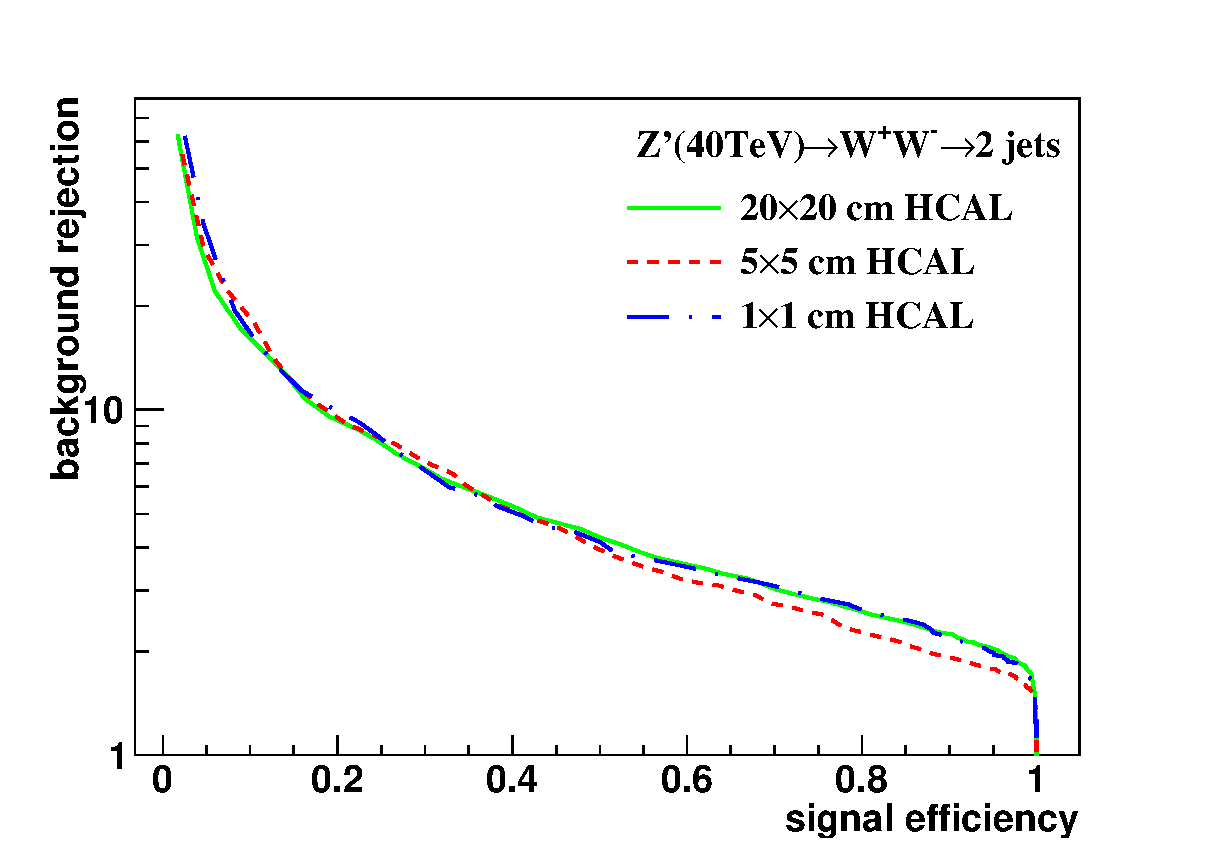
\includegraphics[width=0.43\textwidth]{figs/A_Cluster_mass_sdb2_40tev_eff_1_central_fix_at_Median_bin_ww_qq_log_no_UOF.eps}
 }
\end{center}
\caption{
The ROC curves of soft drop mass selection for $\beta$=2
with 5, 10, 20, and 40~TeV c.m. energies. 
Three different detector cell sizes are compared: 20$\times$20, 
5$\times$5, and 1$\times$1 (cm$\times$cm). 
The signal (background) process is Z'$\rightarrow$WW 
(Z'$\rightarrow$q$\bar{\mathrm{q}}$).
}
\label{fig:cluster_mass_sdb2_ww_ROC}
\end{figure}


\begin{figure}
\begin{center}
   \subfigure[5~TeV at 20$\times$20 (cm$\times$cm) with cluster] {
   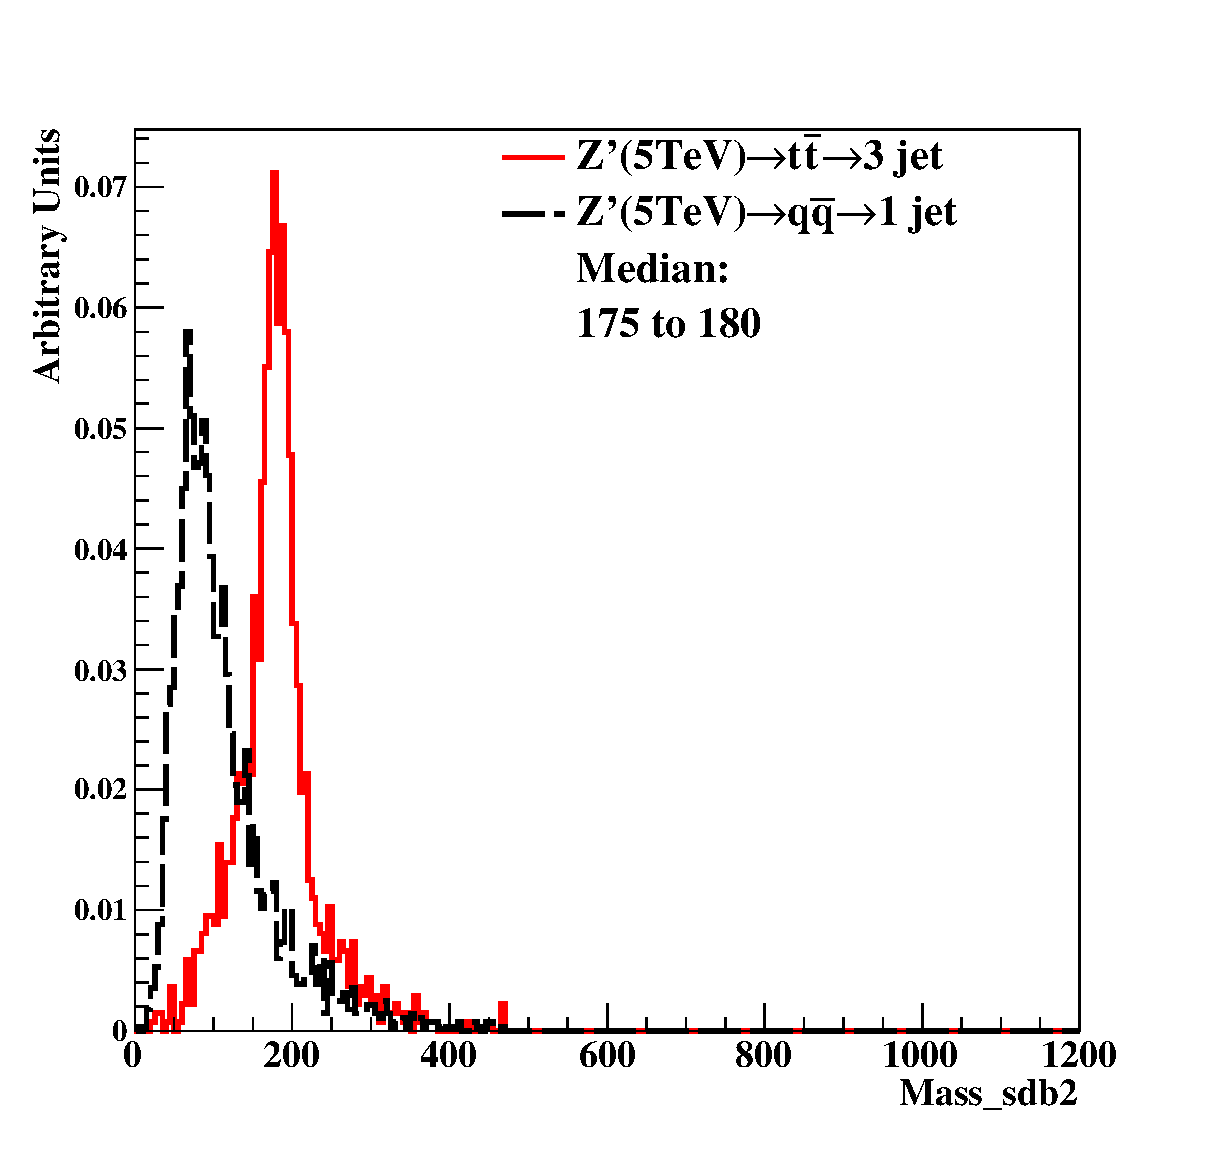
\includegraphics[width=0.22\textwidth]{figs/Dis_cluster_012_mass_sdb2_tt_5tev_04_tt_1200_no_UOF.eps}
   }
      \subfigure[10~TeV at 20$\times$20 (cm$\times$cm) with cluster] {
   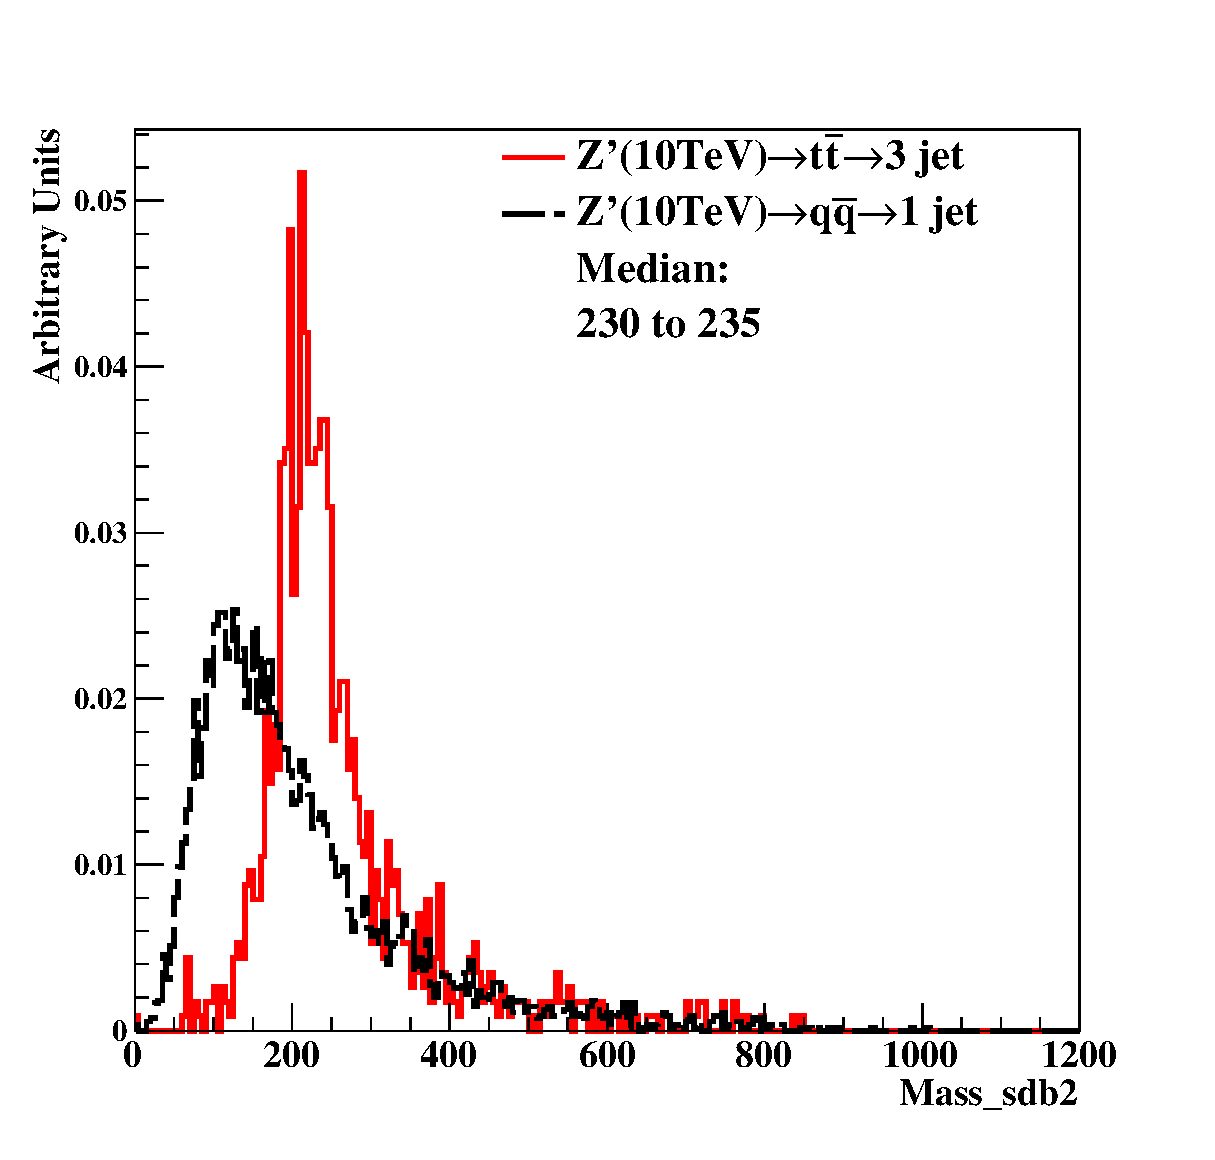
\includegraphics[width=0.22\textwidth]{figs/Dis_cluster_010_mass_sdb2_tt_10tev_04_tt_1200_no_UOF.eps}
   }
   \subfigure[20~TeV at 20$\times$20 (cm$\times$cm) with cluster] {
   \includegraphics[width=0.22\textwidth]{figs/Dis_cluster_010_mass_sdb2_tt_20tev_04_tt_2400_no_UOF.eps}
   }
    \subfigure[40~TeV at 20$\times$20 (cm$\times$cm) with cluster] {
   \includegraphics[width=0.22\textwidth]{figs/Dis_cluster_010_mass_sdb2_tt_40tev_04_tt_2400_no_UOF.eps}
   }
   \subfigure[5~TeV at 5$\times$5 (cm$\times$cm) with cluster] {
   \includegraphics[width=0.22\textwidth]{figs/Dis_cluster_009_mass_sdb2_tt_5tev_04_tt_1200_no_UOF.eps}
   }
   \subfigure[10~TeV at 5$\times$5 (cm$\times$cm) with cluster] {
   \includegraphics[width=0.22\textwidth]{figs/Dis_cluster_009_mass_sdb2_tt_10tev_04_tt_1200_no_UOF.eps}
   }
   \subfigure[20~TeV at 5$\times$5 (cm$\times$cm) with cluster] {
   \includegraphics[width=0.22\textwidth]{figs/Dis_cluster_009_mass_sdb2_tt_20tev_04_tt_2400_no_UOF.eps}\hfill
   }
      \subfigure[40~TeV at 5$\times$5 (cm$\times$cm) with cluster] {
   \includegraphics[width=0.22\textwidth]{figs/Dis_cluster_009_mass_sdb2_tt_40tev_04_tt_2400_no_UOF.eps}\hfill
   }
   \subfigure[5~TeV at 1$\times$1 (cm$\times$cm) with cluster] {
   \includegraphics[width=0.22\textwidth]{figs/Dis_cluster_012_mass_sdb2_tt_5tev_04_tt_1200_no_UOF.eps}\hfill
   }
    \subfigure[10~TeV at 1$\times$1 (cm$\times$cm) with cluster] {
   \includegraphics[width=0.22\textwidth]{figs/Dis_cluster_012_mass_sdb2_tt_10tev_04_tt_1200_no_UOF.eps}
   }
   \subfigure[20~TeV at 1$\times$1 (cm$\times$cm) with cluster] {
   \includegraphics[width=0.22\textwidth]{figs/Dis_cluster_012_mass_sdb2_tt_20tev_04_tt_2400_no_UOF.eps}\hfill
   }
      \subfigure[40~TeV at 1$\times$1 (cm$\times$cm) with cluster] {
   \includegraphics[width=0.22\textwidth]{figs/Dis_cluster_012_mass_sdb2_tt_40tev_04_tt_2400_no_UOF.eps}
   }
\end{center}
\caption{
Distributions of soft drop mass for $\beta$=2, with 5, 10, 20, and 
40~TeV c.m. energies and three different detector cell sizes: 20$\times$20, 
5$\times$5, and 1$\times$1 (cm$\times$cm). The signal (background) process is 
Z'$\rightarrow$t$\bar{\mathrm{t}}$ (Z'$\rightarrow$q$\bar{\mathrm{q}}$).
}
\label{fig:cluster_mass_sdb2_tt}
\end{figure}


\begin{figure}
\begin{center}
  \subfigure[Central at Median($20\times20$=,$5\times5$=,$1\times1$=) change width with cluster at 5~TeV] {
  \includegraphics[width=0.43\textwidth]{figs/A_Cluster_mass_sdb2_5tev_eff_1_central_fix_at_Median_bin_tt_qq_log_no_UOF.eps}
  }
  \subfigure[Central at Median($20\times20$=,$5\times5$=,$1\times1$=) change width with cluster at 10~TeV] {
  \includegraphics[width=0.43\textwidth]{figs/A_Cluster_mass_sdb2_10tev_eff_1_central_fix_at_Median_bin_tt_qq_log_no_UOF.eps}
  }
 \subfigure[Central at Median($20\times20$=,$5\times5$=,$1\times1$=) change width with cluster at 20~TeV] {
 \includegraphics[width=0.43\textwidth]{figs/A_Cluster_mass_sdb2_20tev_eff_1_central_fix_at_Median_bin_tt_qq_log_no_UOF.eps}
 }
 \subfigure[Central at Median($20\times20$=,$5\times5$=,$1\times1$=) change width with cluster at 40~TeV] {
 \includegraphics[width=0.43\textwidth]{figs/A_Cluster_mass_sdb2_40tev_eff_1_central_fix_at_Median_bin_tt_qq_log_no_UOF.eps}
 }
\end{center}
\caption{
The ROC curves of soft drop mass selection for $\beta$=2
with 5, 10, 20, and 40~TeV c.m. energies. 
Three different detector cell sizes are compared: 20$\times$20, 
5$\times$5, and 1$\times$1 (cm$\times$cm). 
The signal (background) process is Z'$\rightarrow$t$\bar{\mathrm{t}}$
(Z'$\rightarrow$q$\bar{\mathrm{q}}$).
}
\label{fig:cluster_mass_sdb2_tt_ROC}
\end{figure}





